%%%%%%%%%%%%%%%%%%%%%%%%%%%%%%%%%%%%%%%%%%%%%%%%%%%%%%%%%%%%%%
%%%%%%%%%%%%%%%%%%%%%%%%%%%%%%%%%%%%%%%%%%%%%%%%%%%%%%%%%%%%%%
%%%%%%%%%%%%%%%%%%%%%%%%%%%%%%%%%%%%%%%%%%%%%%%%%%%%%%%%%%%%%%

\subsection{Data pipeline}

\begin{table}[H]
\centering
\caption{Chronological overview of the data processing and modelling pipeline.}
\label{tab:data_processing_pipeline}
\small
\begin{tabularx}{\linewidth}{clX}
\toprule
\textbf{Step} & \textbf{Stage} & \textbf{Description} \\
\midrule
1  & Download data & Download monthly Dukascopy tick data for each currency leg. \\
2  & Separate quote sides & Store bid and ask files separately for each asset and month. \\
3  & Load files & Load the relevant parquet files into Python. \\
4  & Filter observations & Restrict the data to the chosen trading days and active trading hours. \\
5  & Sort timestamps & Sort all bid and ask quote streams chronologically. \\
6  & Align bid--ask quotes & Merge bid and ask streams within each asset using backward as-of alignment. \\
7  & Compute mid-prices & Compute mid-prices from bid and ask quotes. \\
8  & Compute half-spreads & Compute half-spreads in basis points for each asset. \\
9  & Aggregate bars & Aggregate raw ticks into event-based volume bars. \\
10 & Preserve continuity & Carry cumulative volume across monthly file boundaries. \\
11 & Synchronize pair legs & Merge the two assets into synchronized pair-level observations. \\
12 & Compute log-prices & Transform mid-prices into log-prices. \\
13 & Compute returns & Compute one-bar log returns for both assets. \\
14 & Estimate hedge ratio & Estimate static and rolling hedge ratios between the two log-price series. \\
15 & Construct spread & Construct the log spread using the estimated hedge ratio. \\
16 & Standardize spread & Compute rolling spread mean, rolling spread volatility, and the spread $z$-score. \\
17 & Compute spread returns & Compute hedged spread returns using lagged hedge ratios. \\
18 & Run diagnostics & Produce descriptive, liquidity, correlation, and cointegration diagnostics. \\
19 & Fit AR model & Estimate the autoregressive benchmark model. \\
20 & Fit Markov model & Estimate hidden Markov regime probabilities using spread returns. \\
21 & Walk-forward prediction & Generate out-of-sample signals and regime probabilities. \\
22 & Optimize rules & Use walk-forward optimization to select trading thresholds. \\
23 & Backtest strategies & Evaluate baseline, AR-filtered, and MS-AR strategies net of costs. \\
24 & Summarize performance & Produce tearsheets, figures, and strategy comparison tables. \\
\bottomrule
\end{tabularx}
\end{table}

%%%%%%%%%%%%%%%%%%%%%%%%%%%%%%%%%%%%%%%%%%%%%%%%%%%%%%%%%%%%%%
%%%%%%%%%%%%%%%%%%%%%%%%%%%%%%%%%%%%%%%%%%%%%%%%%%%%%%%%%%%%%%
%%%%%%%%%%%%%%%%%%%%%%%%%%%%%%%%%%%%%%%%%%%%%%%%%%%%%%%%%%%%%%

\subsection{Exploratory data analysis}

\subsubsection{AUDUSD/NZDUSD}
\begin{figure}[H]
    \centering
    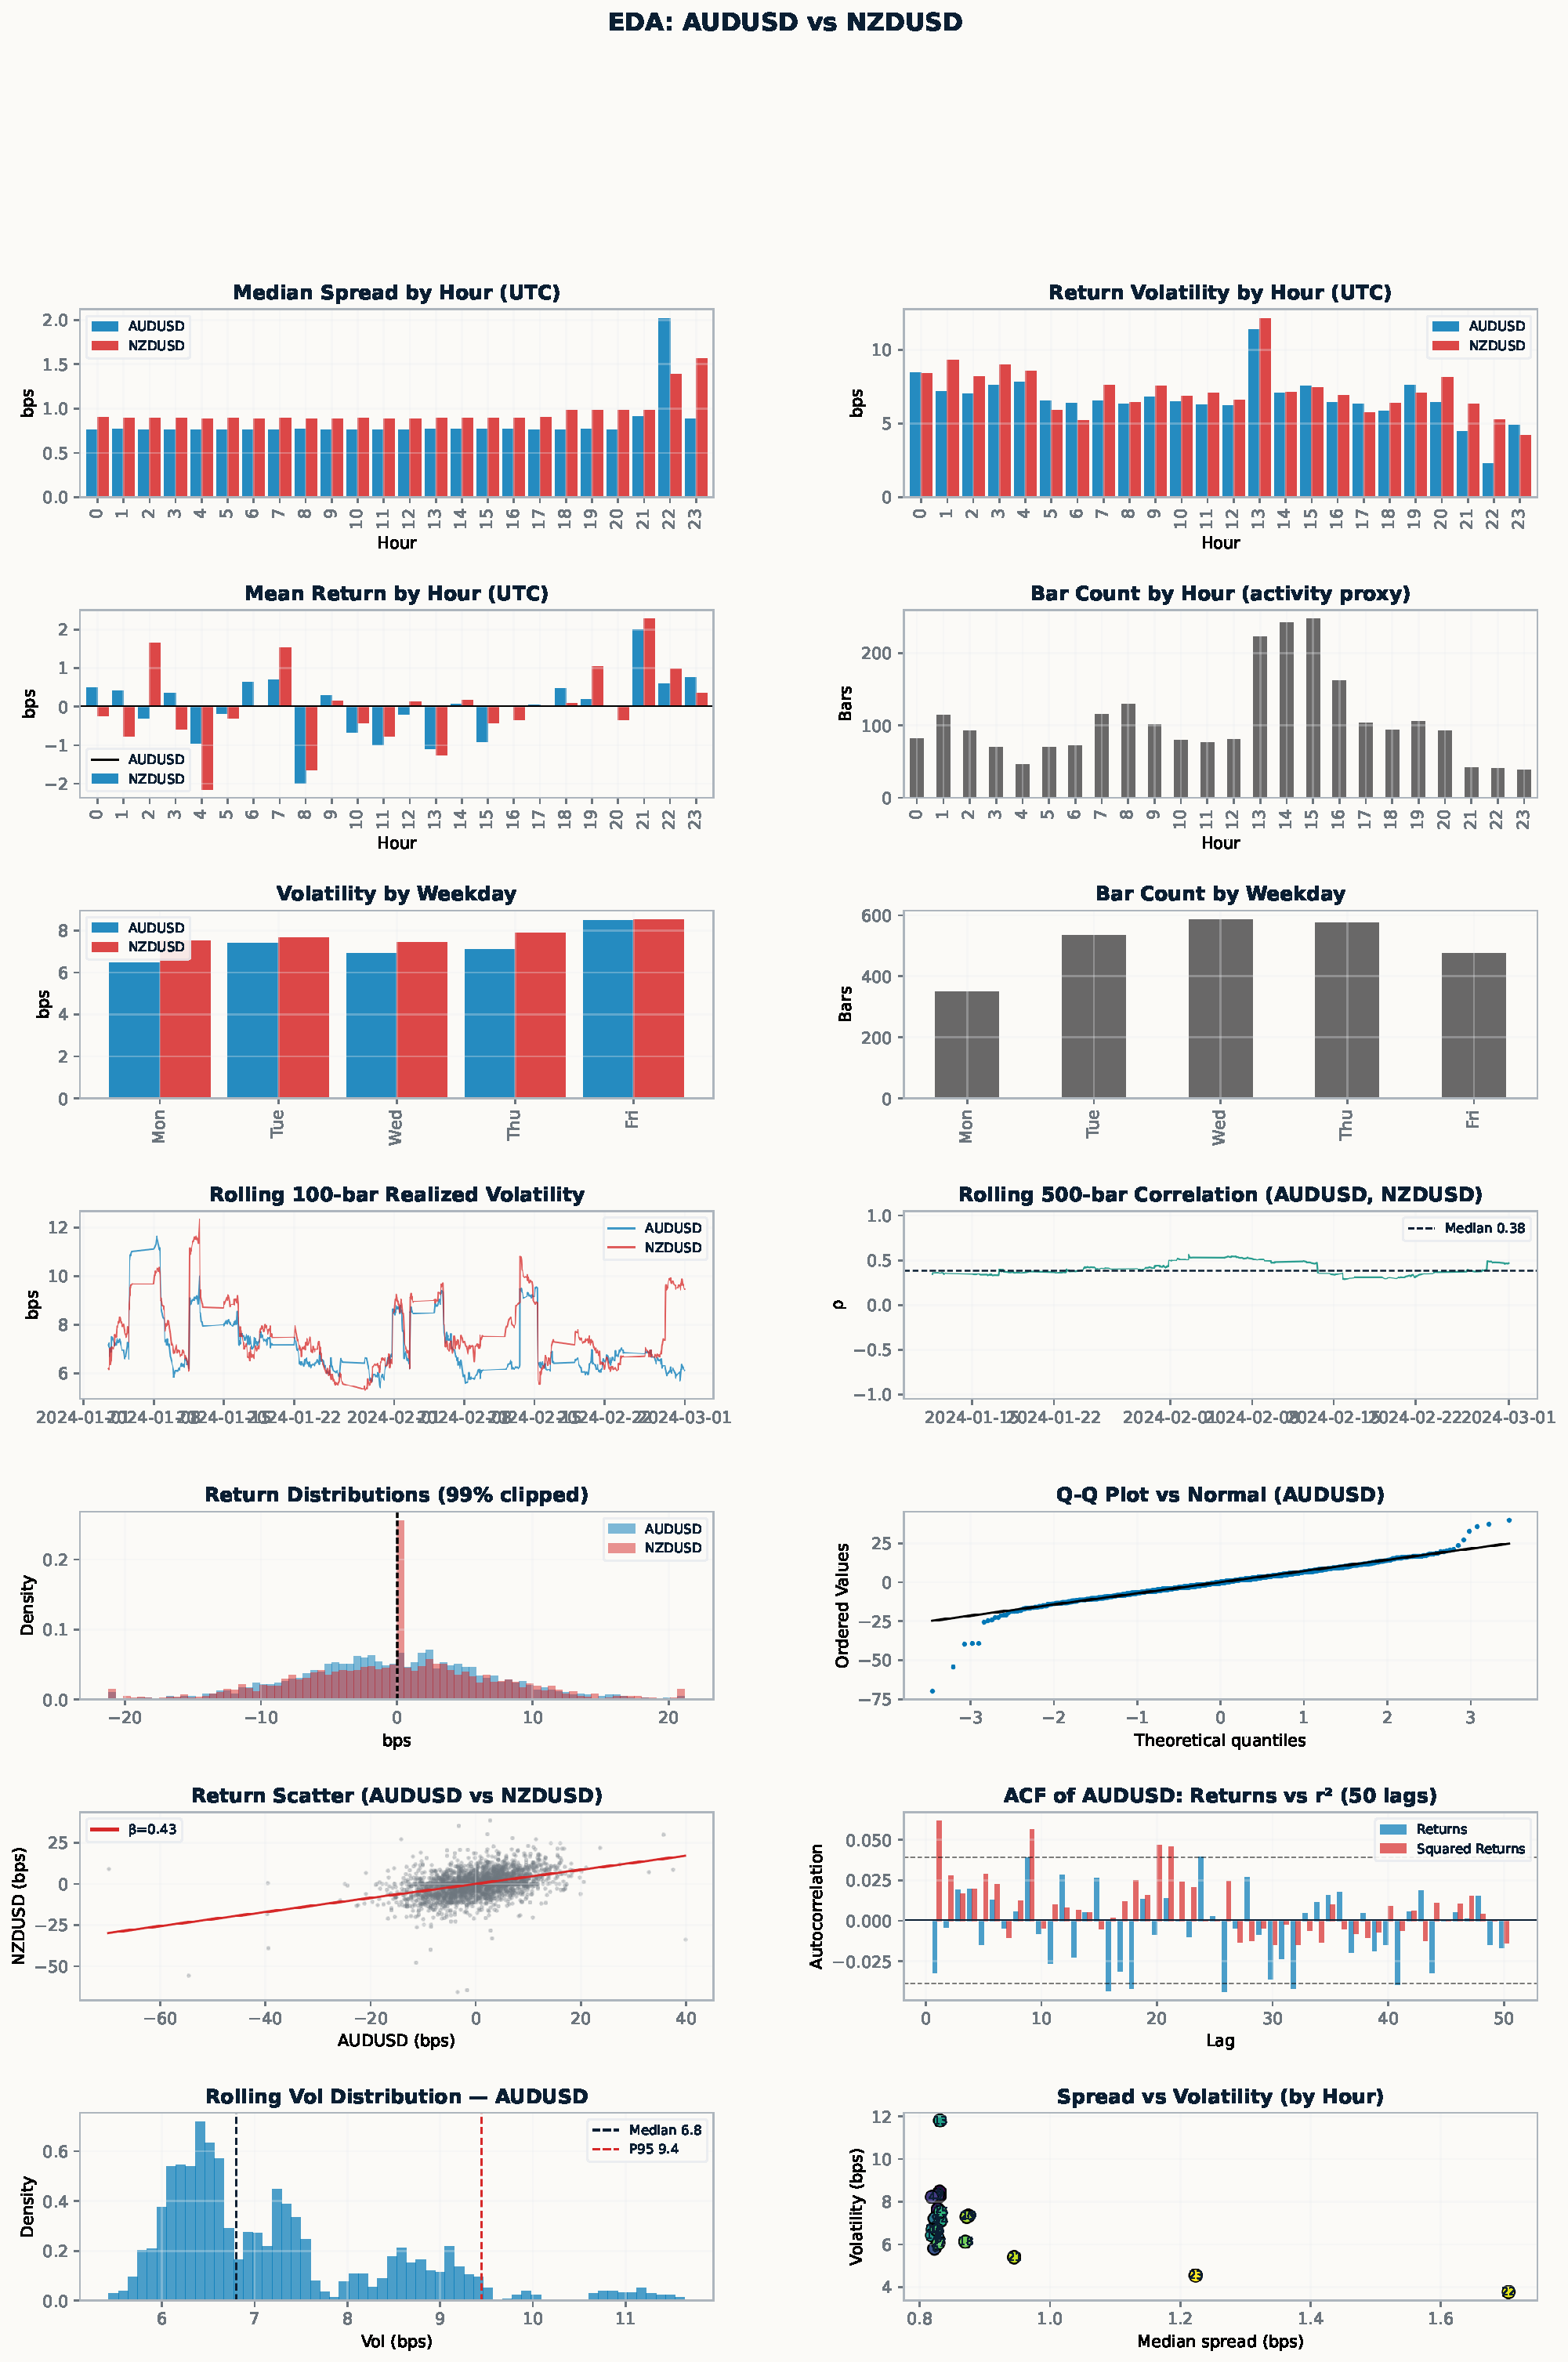
\includegraphics[width=0.85\textwidth]{plots/AUDUSD_NZDUSD_eda.pdf}
    \caption{Exploratory data analysis for AUDUSD/NZDUSD. The figure summarizes intraday spreads, return volatility, mean returns, activity patterns, weekday effects, rolling realized volatility, rolling correlation, return distributions, normality diagnostics, cross-pair return scatter, autocorrelation, rolling volatility distribution, and the relationship between spread and volatility.}
    \label{fig:AUDUSD_NZDUSD_eda}
\end{figure}

\subsubsection{EURNOK/EURSEK}
\begin{figure}[H]
    \centering
    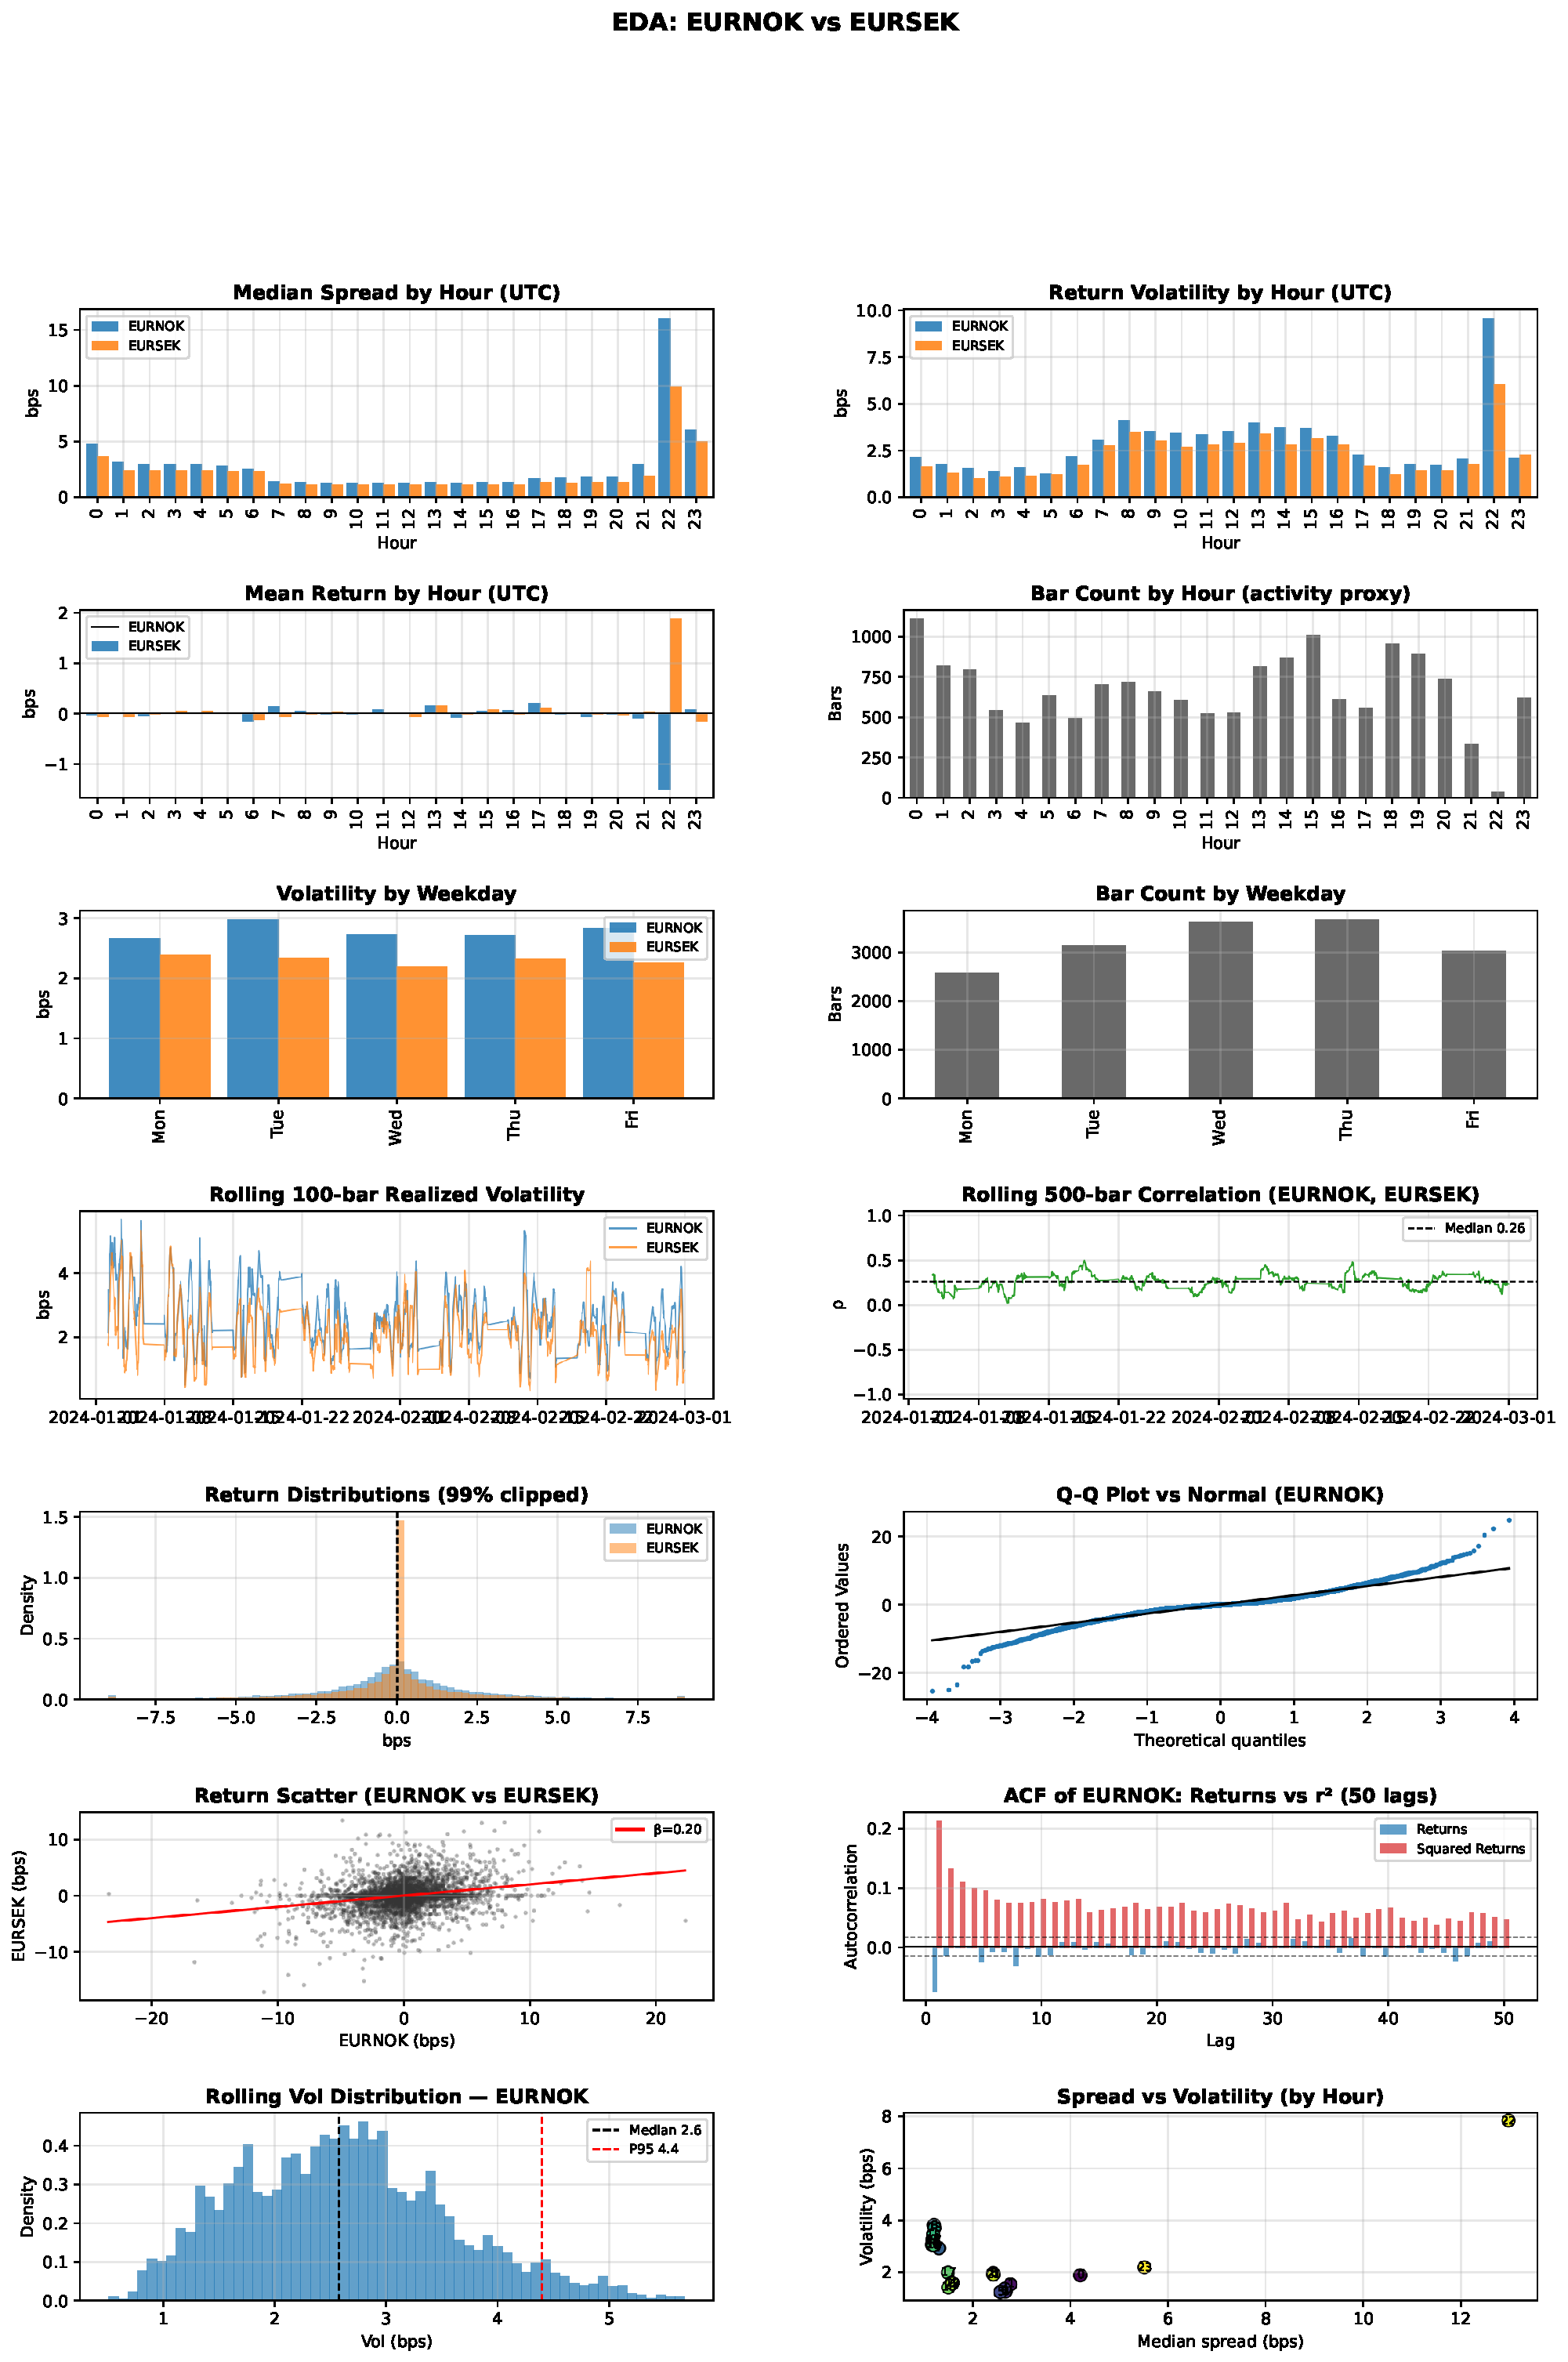
\includegraphics[width=0.85\textwidth]{plots/EURNOK_EURSEK_eda.pdf}
    \caption{Exploratory data analysis for EURNOK/EURSEK. The figure summarizes intraday spreads, volatility, mean returns, bar counts, weekday effects, rolling realized volatility, rolling correlation, distributional features, normality diagnostics, cross-pair return scatter, autocorrelation, rolling volatility, and the spread-volatility relationship.}
    \label{fig:EURNOK_EURSEK_eda}
\end{figure}

\subsubsection{GBPUSD/EURUSD}
\begin{figure}[H]
    \centering
    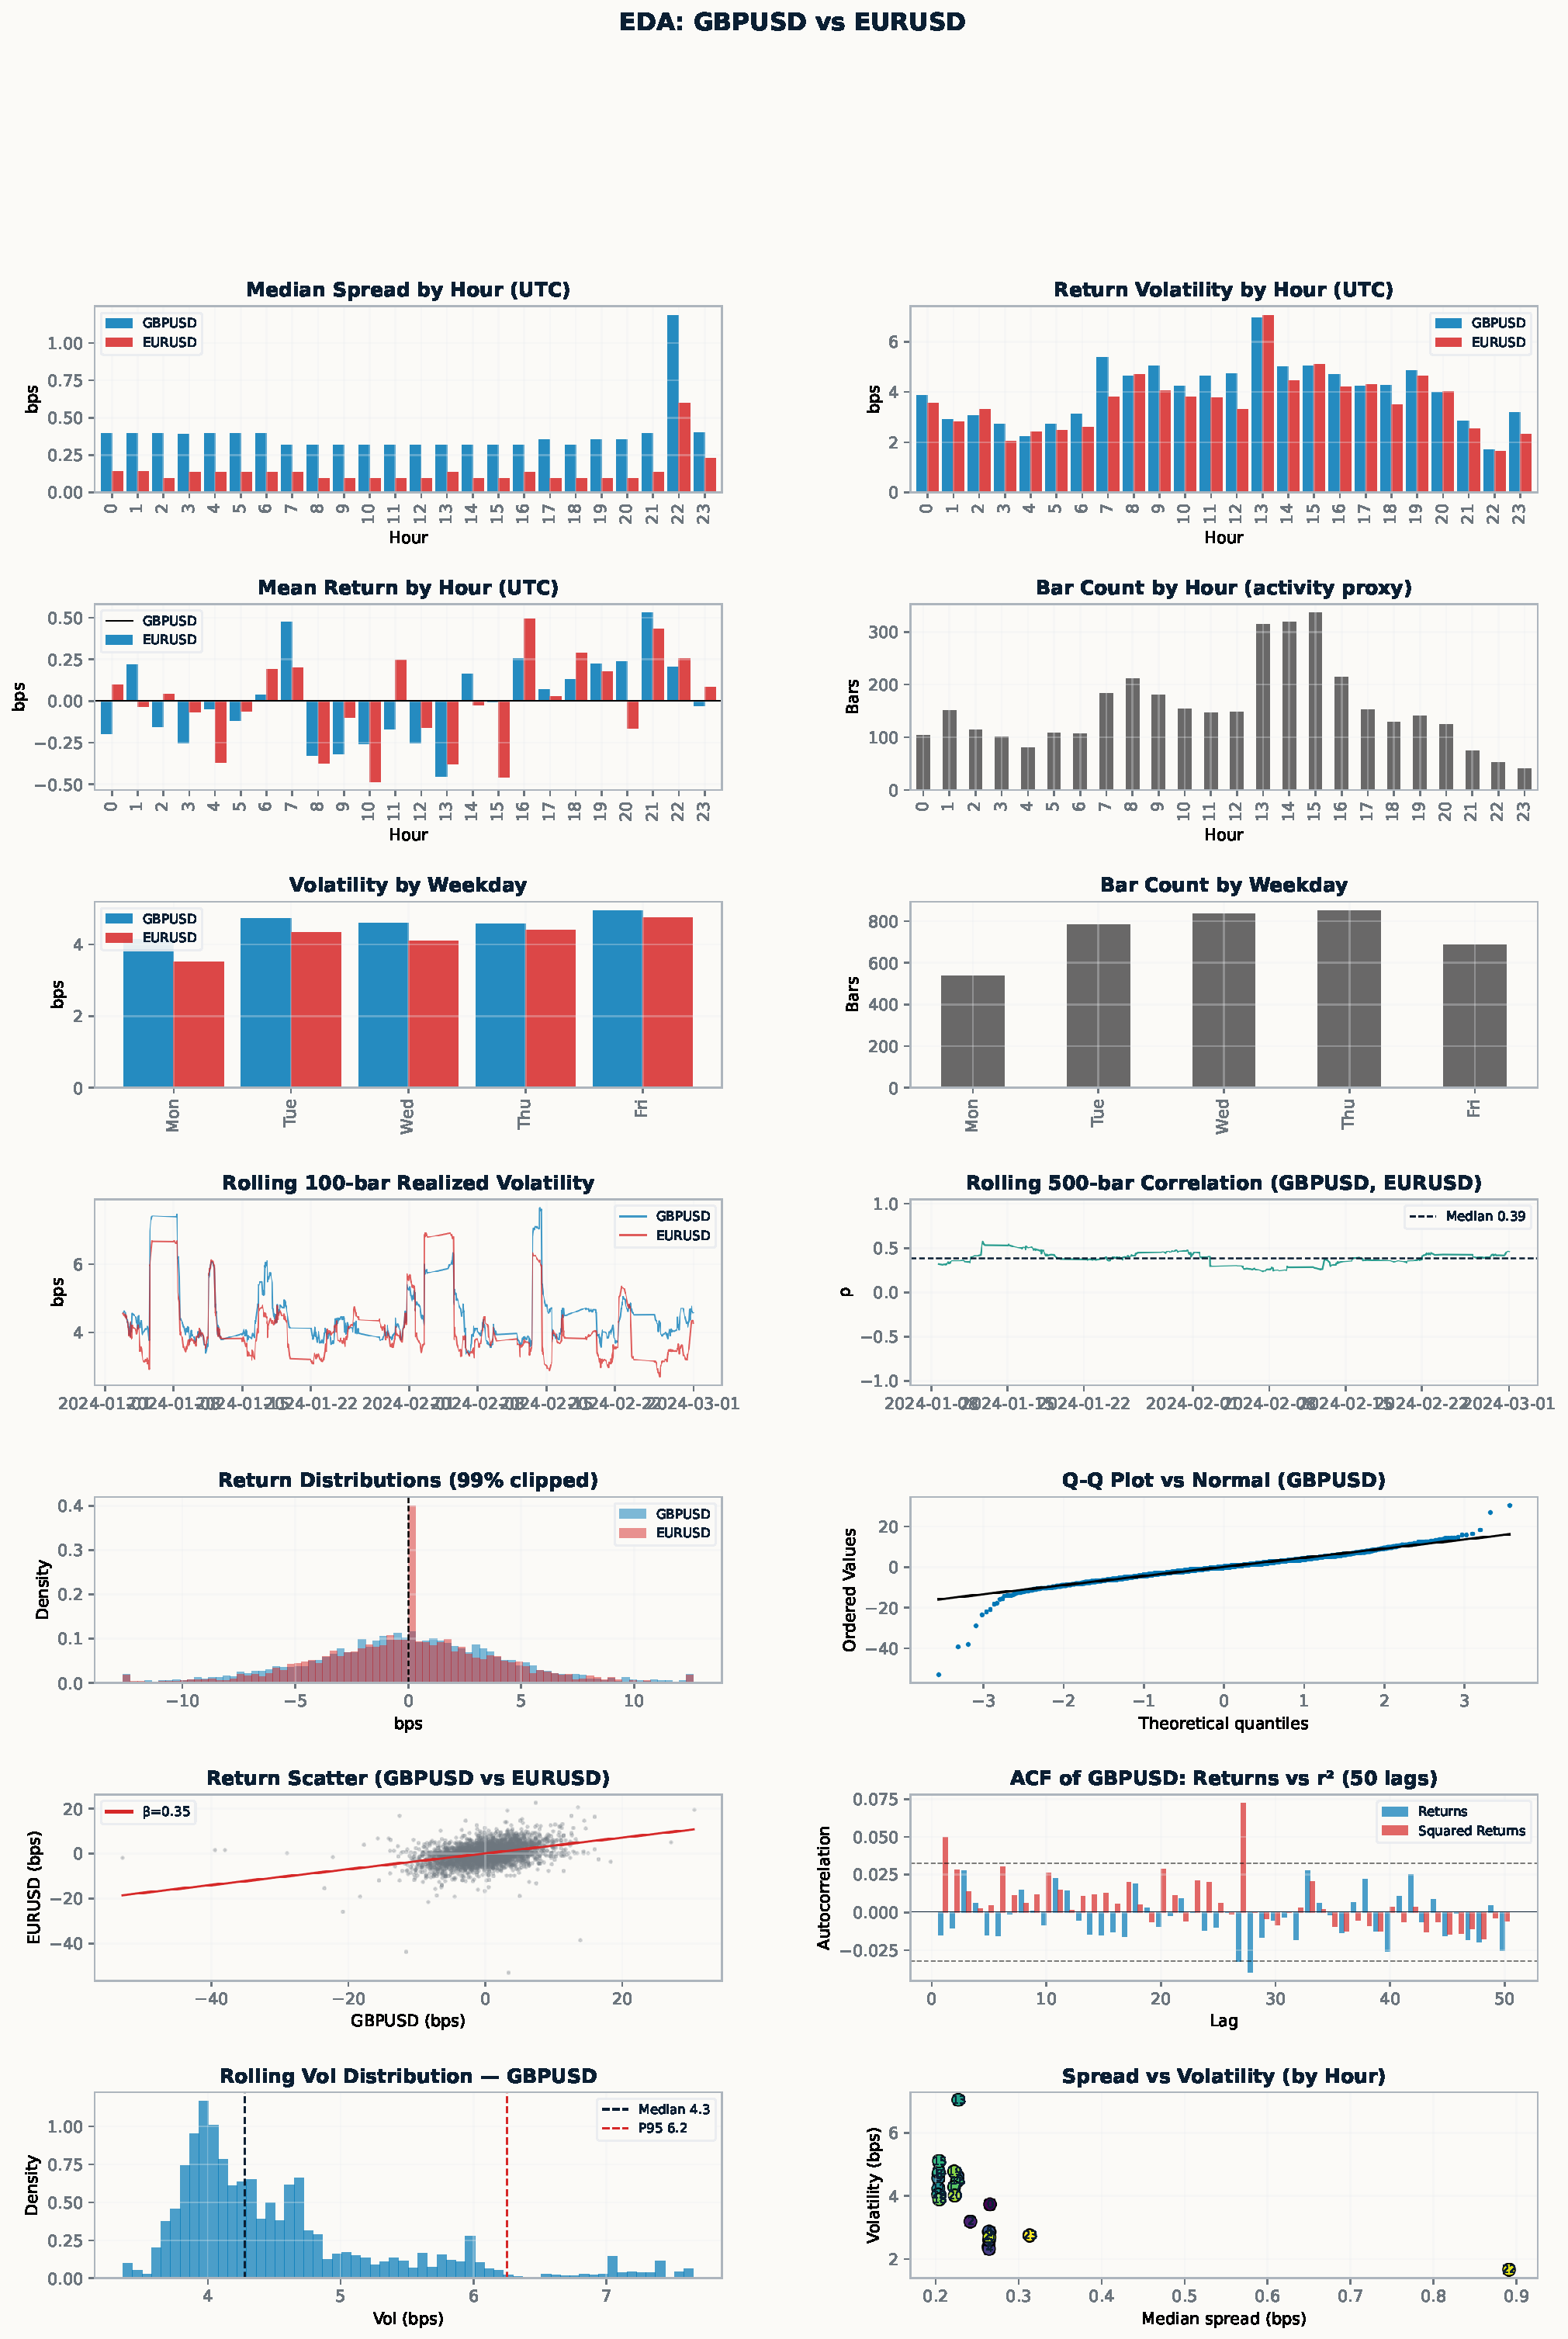
\includegraphics[width=0.85\textwidth]{plots/GBPUSD_EURUSD_eda.pdf}
    \caption{Exploratory data analysis for GBPUSD/EURUSD. The figure summarizes intraday liquidity and volatility patterns, hourly and weekday activity, rolling realized volatility, rolling correlation, return distributions, normality diagnostics, cross-pair return dependence, autocorrelation, and the relationship between spread and volatility.}
    \label{fig:GBPUSD_EURUSD_eda}
\end{figure}

%%%%%%%%%%%%%%%%%%%%%%%%%%%%%%%%%%%%%%%%%%%%%%%%%%%%%%%%%%%%%%
%%%%%%%%%%%%%%%%%%%%%%%%%%%%%%%%%%%%%%%%%%%%%%%%%%%%%%%%%%%%%%
%%%%%%%%%%%%%%%%%%%%%%%%%%%%%%%%%%%%%%%%%%%%%%%%%%%%%%%%%%%%%%

\subsection{Spread diagnostics}

\subsubsection{AUDUSD/NZDUSD}
\begin{figure}[H]
    \centering
    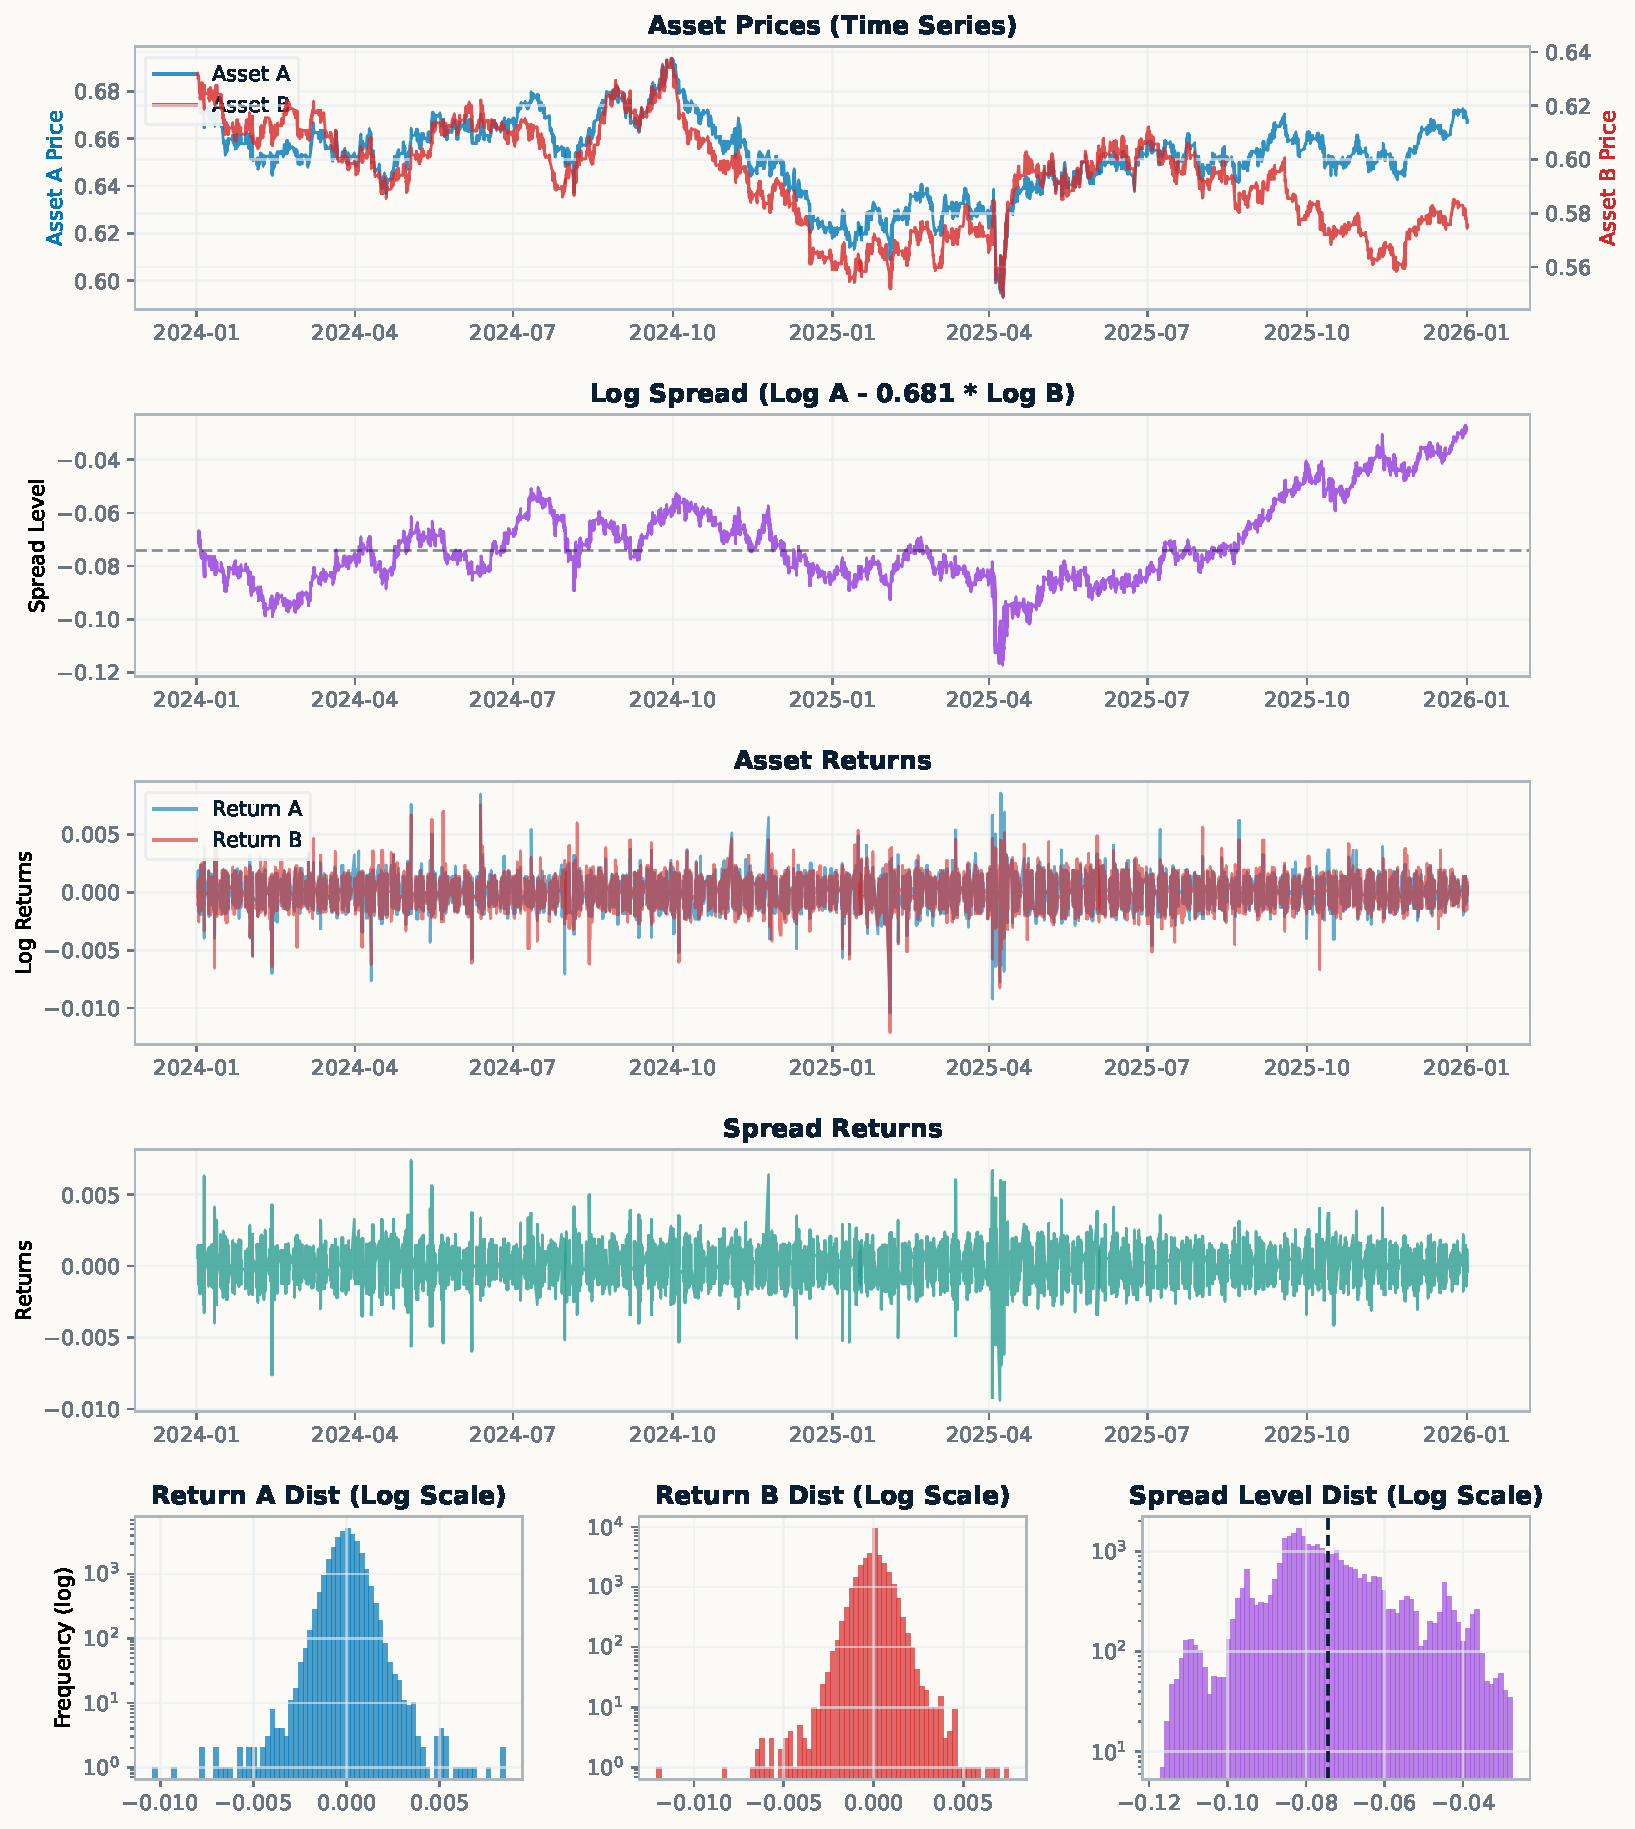
\includegraphics[width=0.9\textwidth]{plots/AUDUSD_NZDUSD_spread_diagnostics.pdf}
    \caption{Spread diagnostics for AUDUSD/NZDUSD. The figure shows the two asset price series, the estimated log spread, asset returns, spread returns, and distributional diagnostics for both returns and spread levels, providing a visual check of the pairs-trading signal construction.}
    \label{fig:AUDUSD_NZDUSD_spread_diagnostics}
\end{figure}

\subsubsection{EURNOK/EURSEK}
\begin{figure}[H]
    \centering
    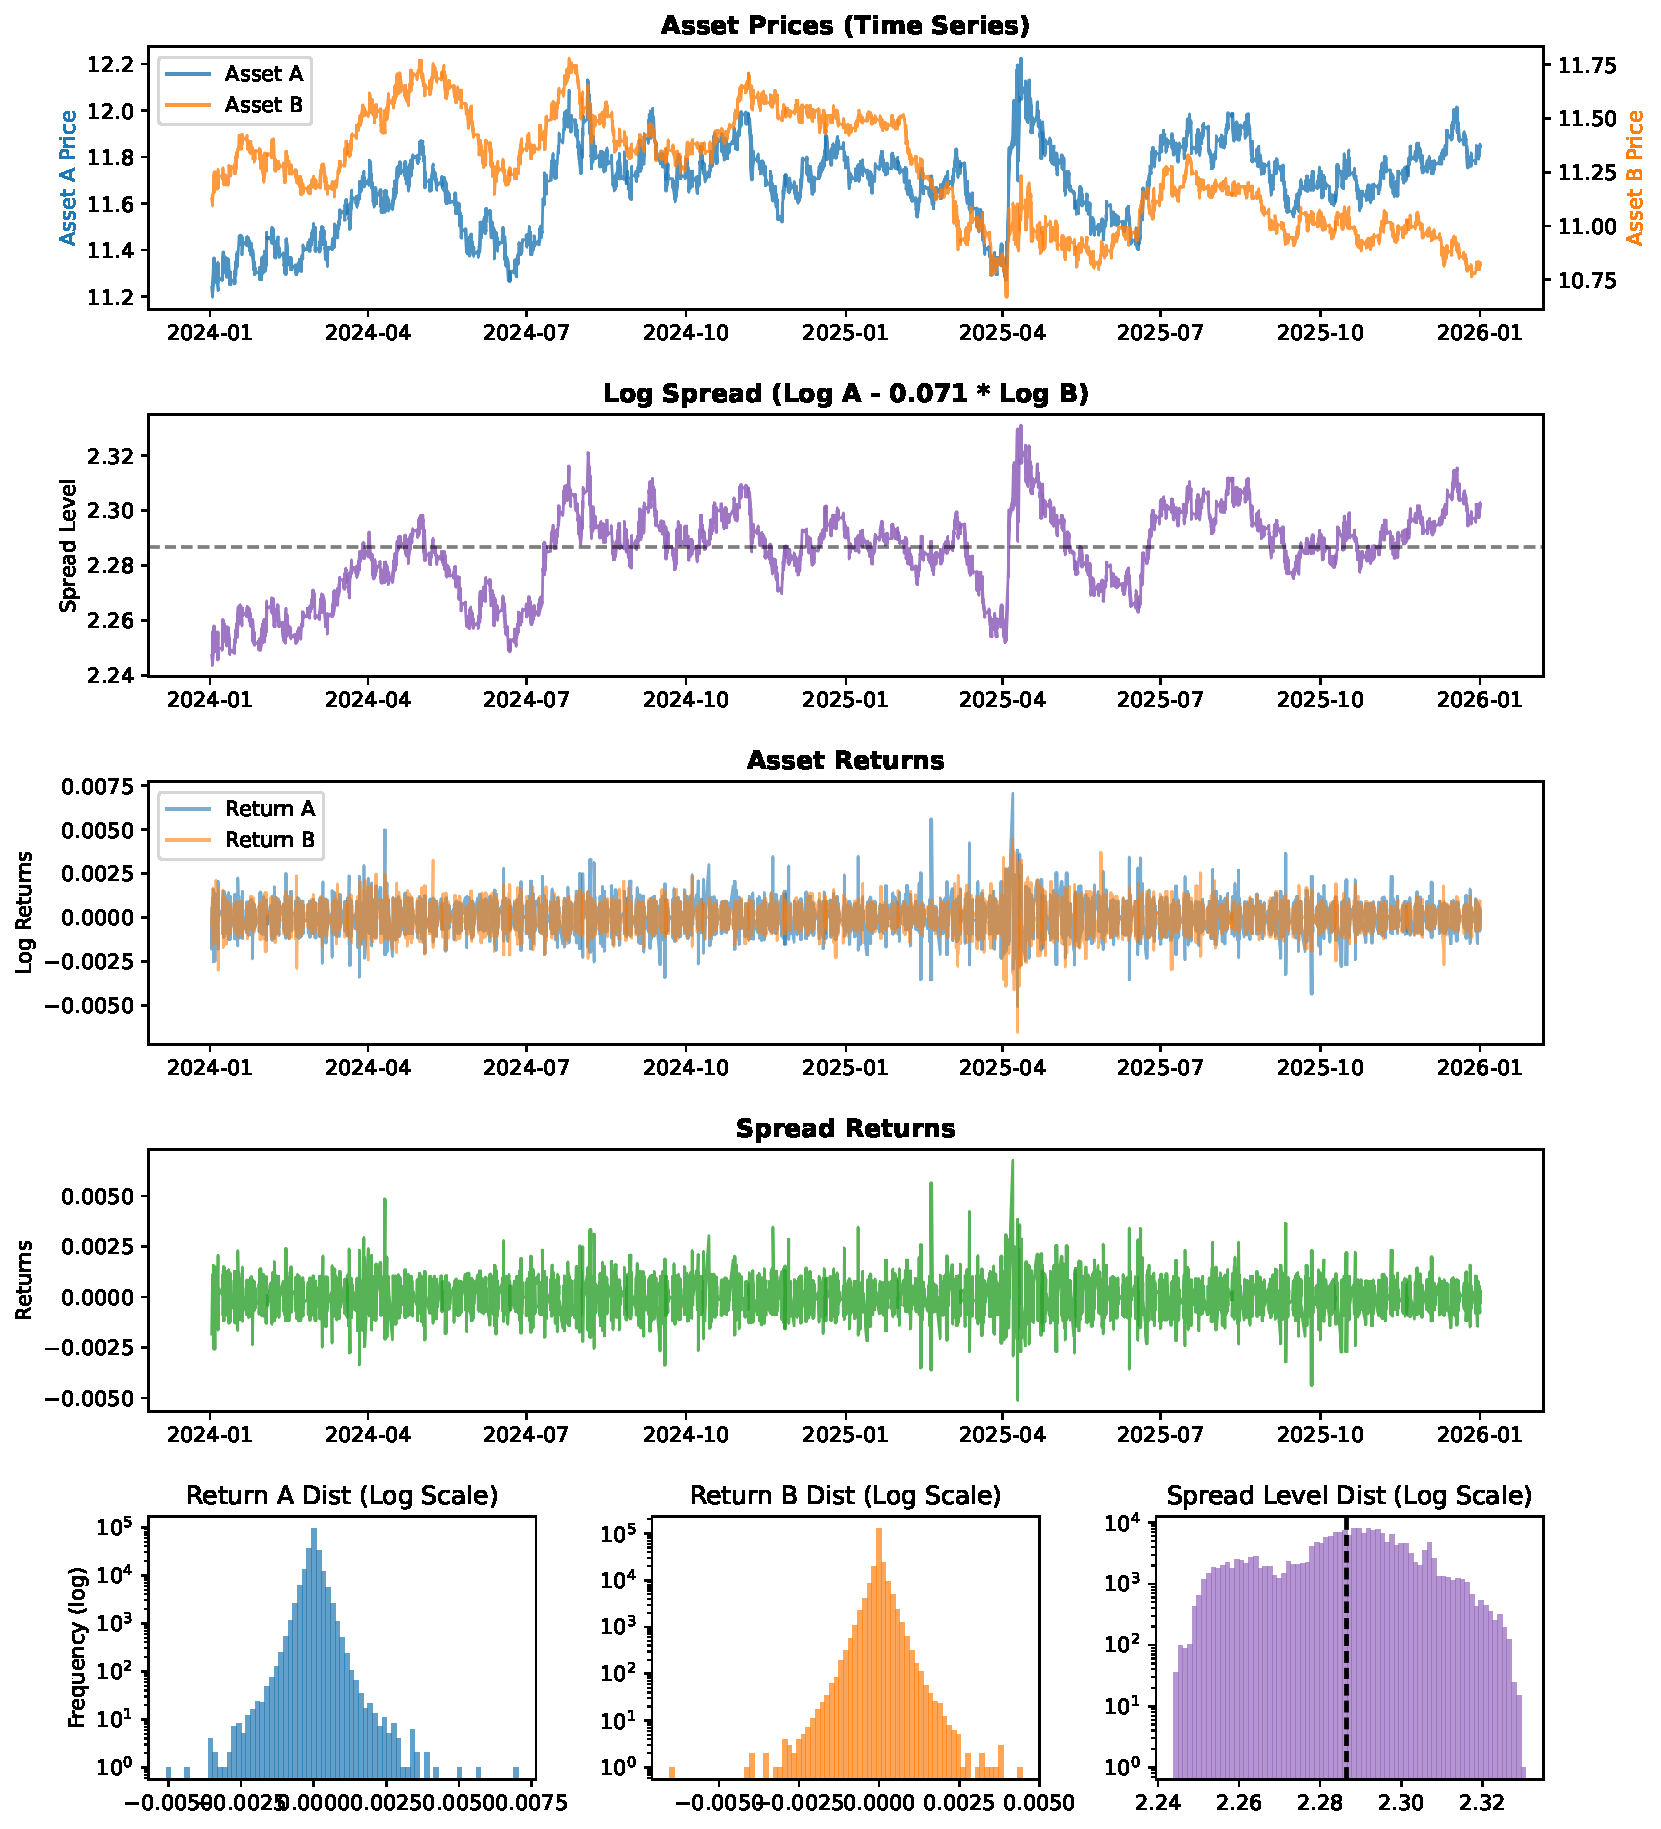
\includegraphics[width=0.9\textwidth]{plots/EURNOK_EURSEK_spread_diagnostics.pdf}
    \caption{Spread diagnostics for EURNOK/EURSEK. The figure presents the asset price paths, fitted log spread, asset returns, spread returns, and distributional diagnostics, allowing visual inspection of spread stability, return asymmetry, and tail behaviour.}
    \label{fig:EURNOK_EURSEK_spread_diagnostics}
\end{figure}

\subsubsection{GBPUSD/EURUSD}
\begin{figure}[H]
    \centering
    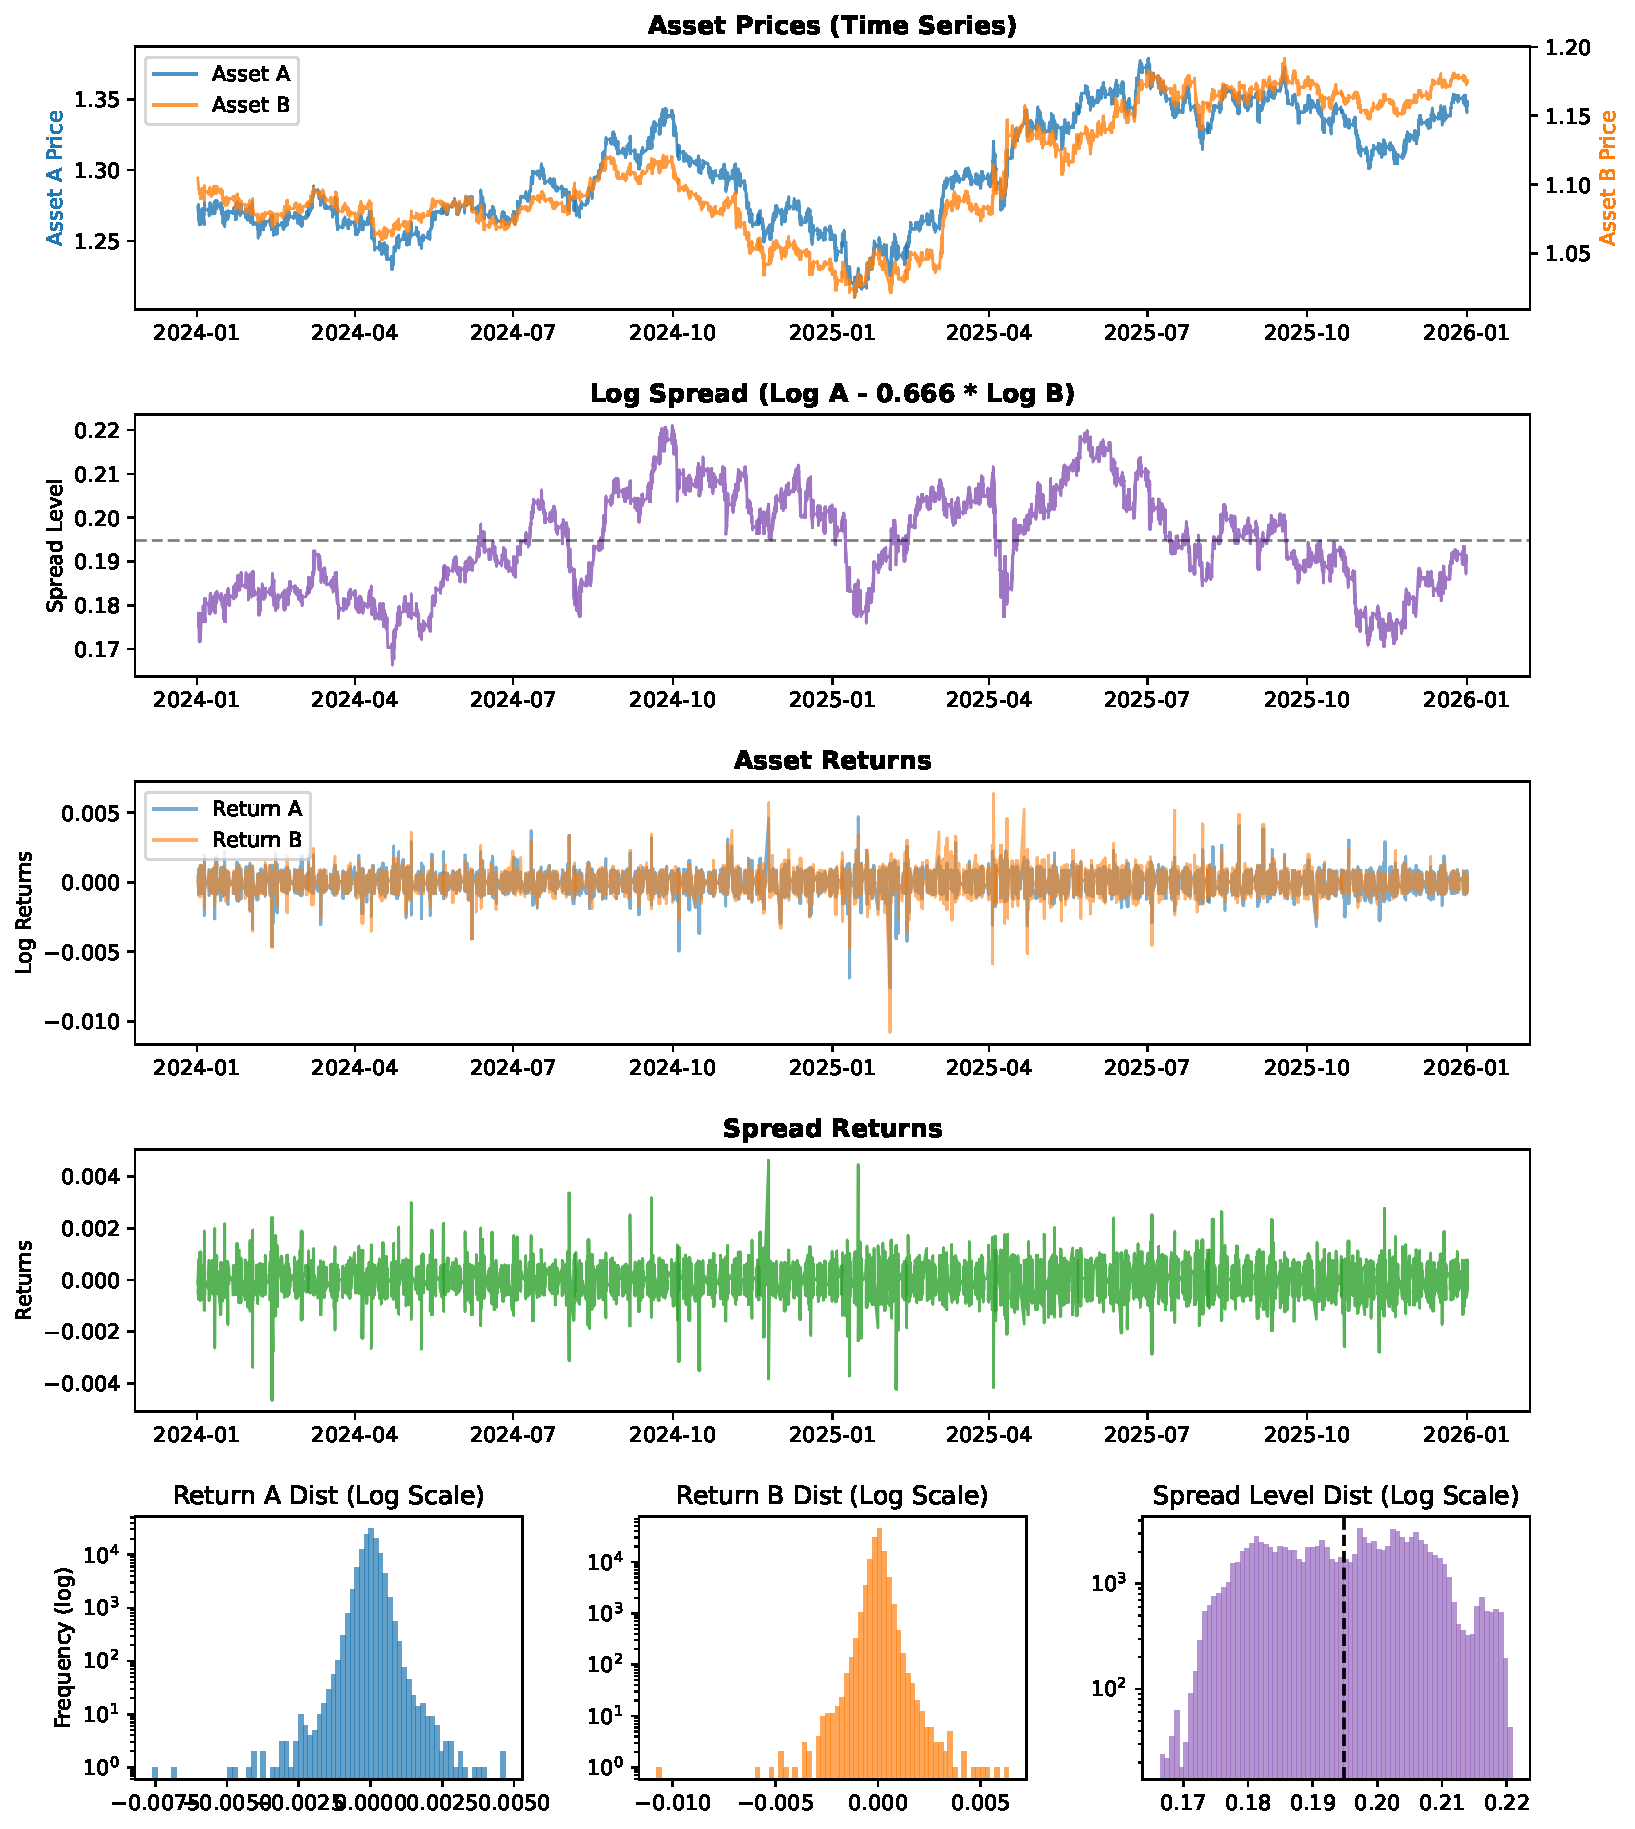
\includegraphics[width=0.9\textwidth]{plots/GBPUSD_EURUSD_spread_diagnostics.pdf}
    \caption{Spread diagnostics for GBPUSD/EURUSD. The figure shows the two asset price series, estimated log spread, asset returns, spread returns, and distributional diagnostics, providing a visual basis for assessing the stability and tradability of the constructed spread.}
    \label{fig:GBPUSD_EURUSD_spread_diagnostics}
\end{figure}

%%%%%%%%%%%%%%%%%%%%%%%%%%%%%%%%%%%%%%%%%%%%%%%%%%%%%%%%%%%%%%
%%%%%%%%%%%%%%%%%%%%%%%%%%%%%%%%%%%%%%%%%%%%%%%%%%%%%%%%%%%%%%
%%%%%%%%%%%%%%%%%%%%%%%%%%%%%%%%%%%%%%%%%%%%%%%%%%%%%%%%%%%%%%


\subsection{Backtest performance}

\subsubsection{AUDUSD/NZDUSD}

\begin{figure}[H]
    \centering
    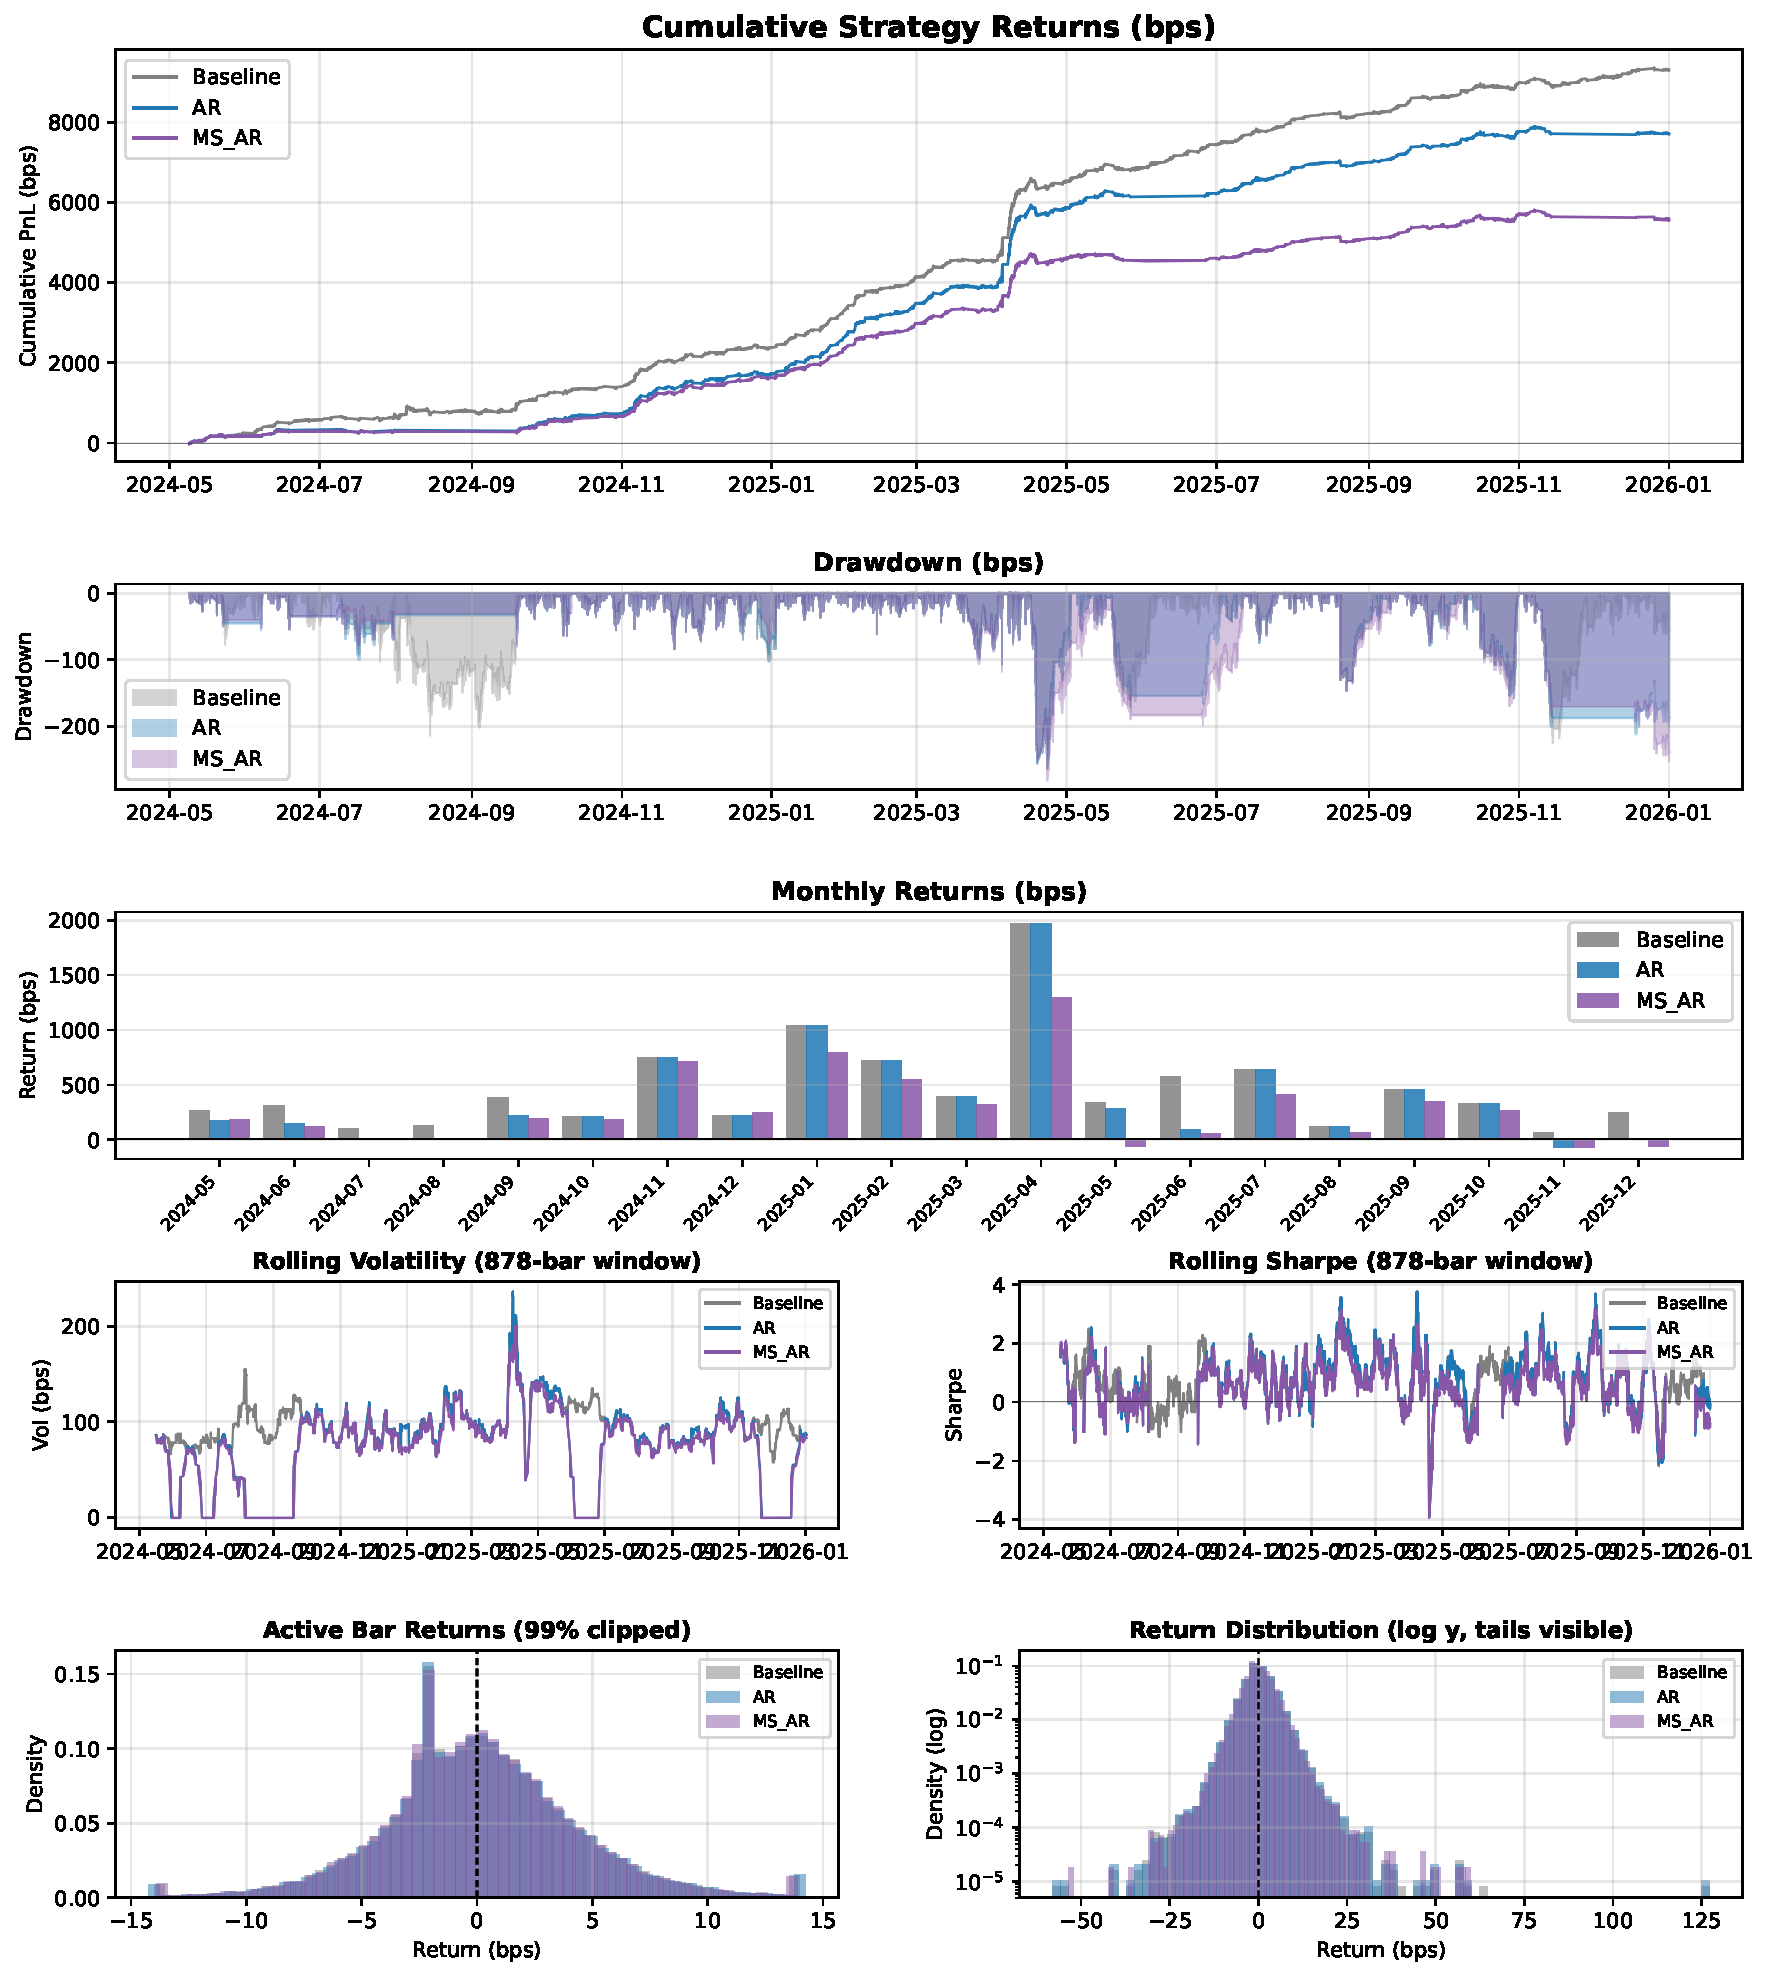
\includegraphics[width=\textwidth]{plots/AUDUSD_NZDUSD_performance.pdf}
    \caption{Backtest performance for AUDUSD/NZDUSD across the baseline, AR, and Markov-switching AR strategies. The figure compares cumulative strategy returns, drawdowns, monthly returns, rolling volatility, rolling Sharpe ratios, active-bar return distributions, and tail behaviour on a log-density scale.}
    \label{fig:AUDUSD_NZDUSD_performance}
\end{figure}

\subsubsection{EURNOK/EURSEK}

\begin{figure}[H]
    \centering
    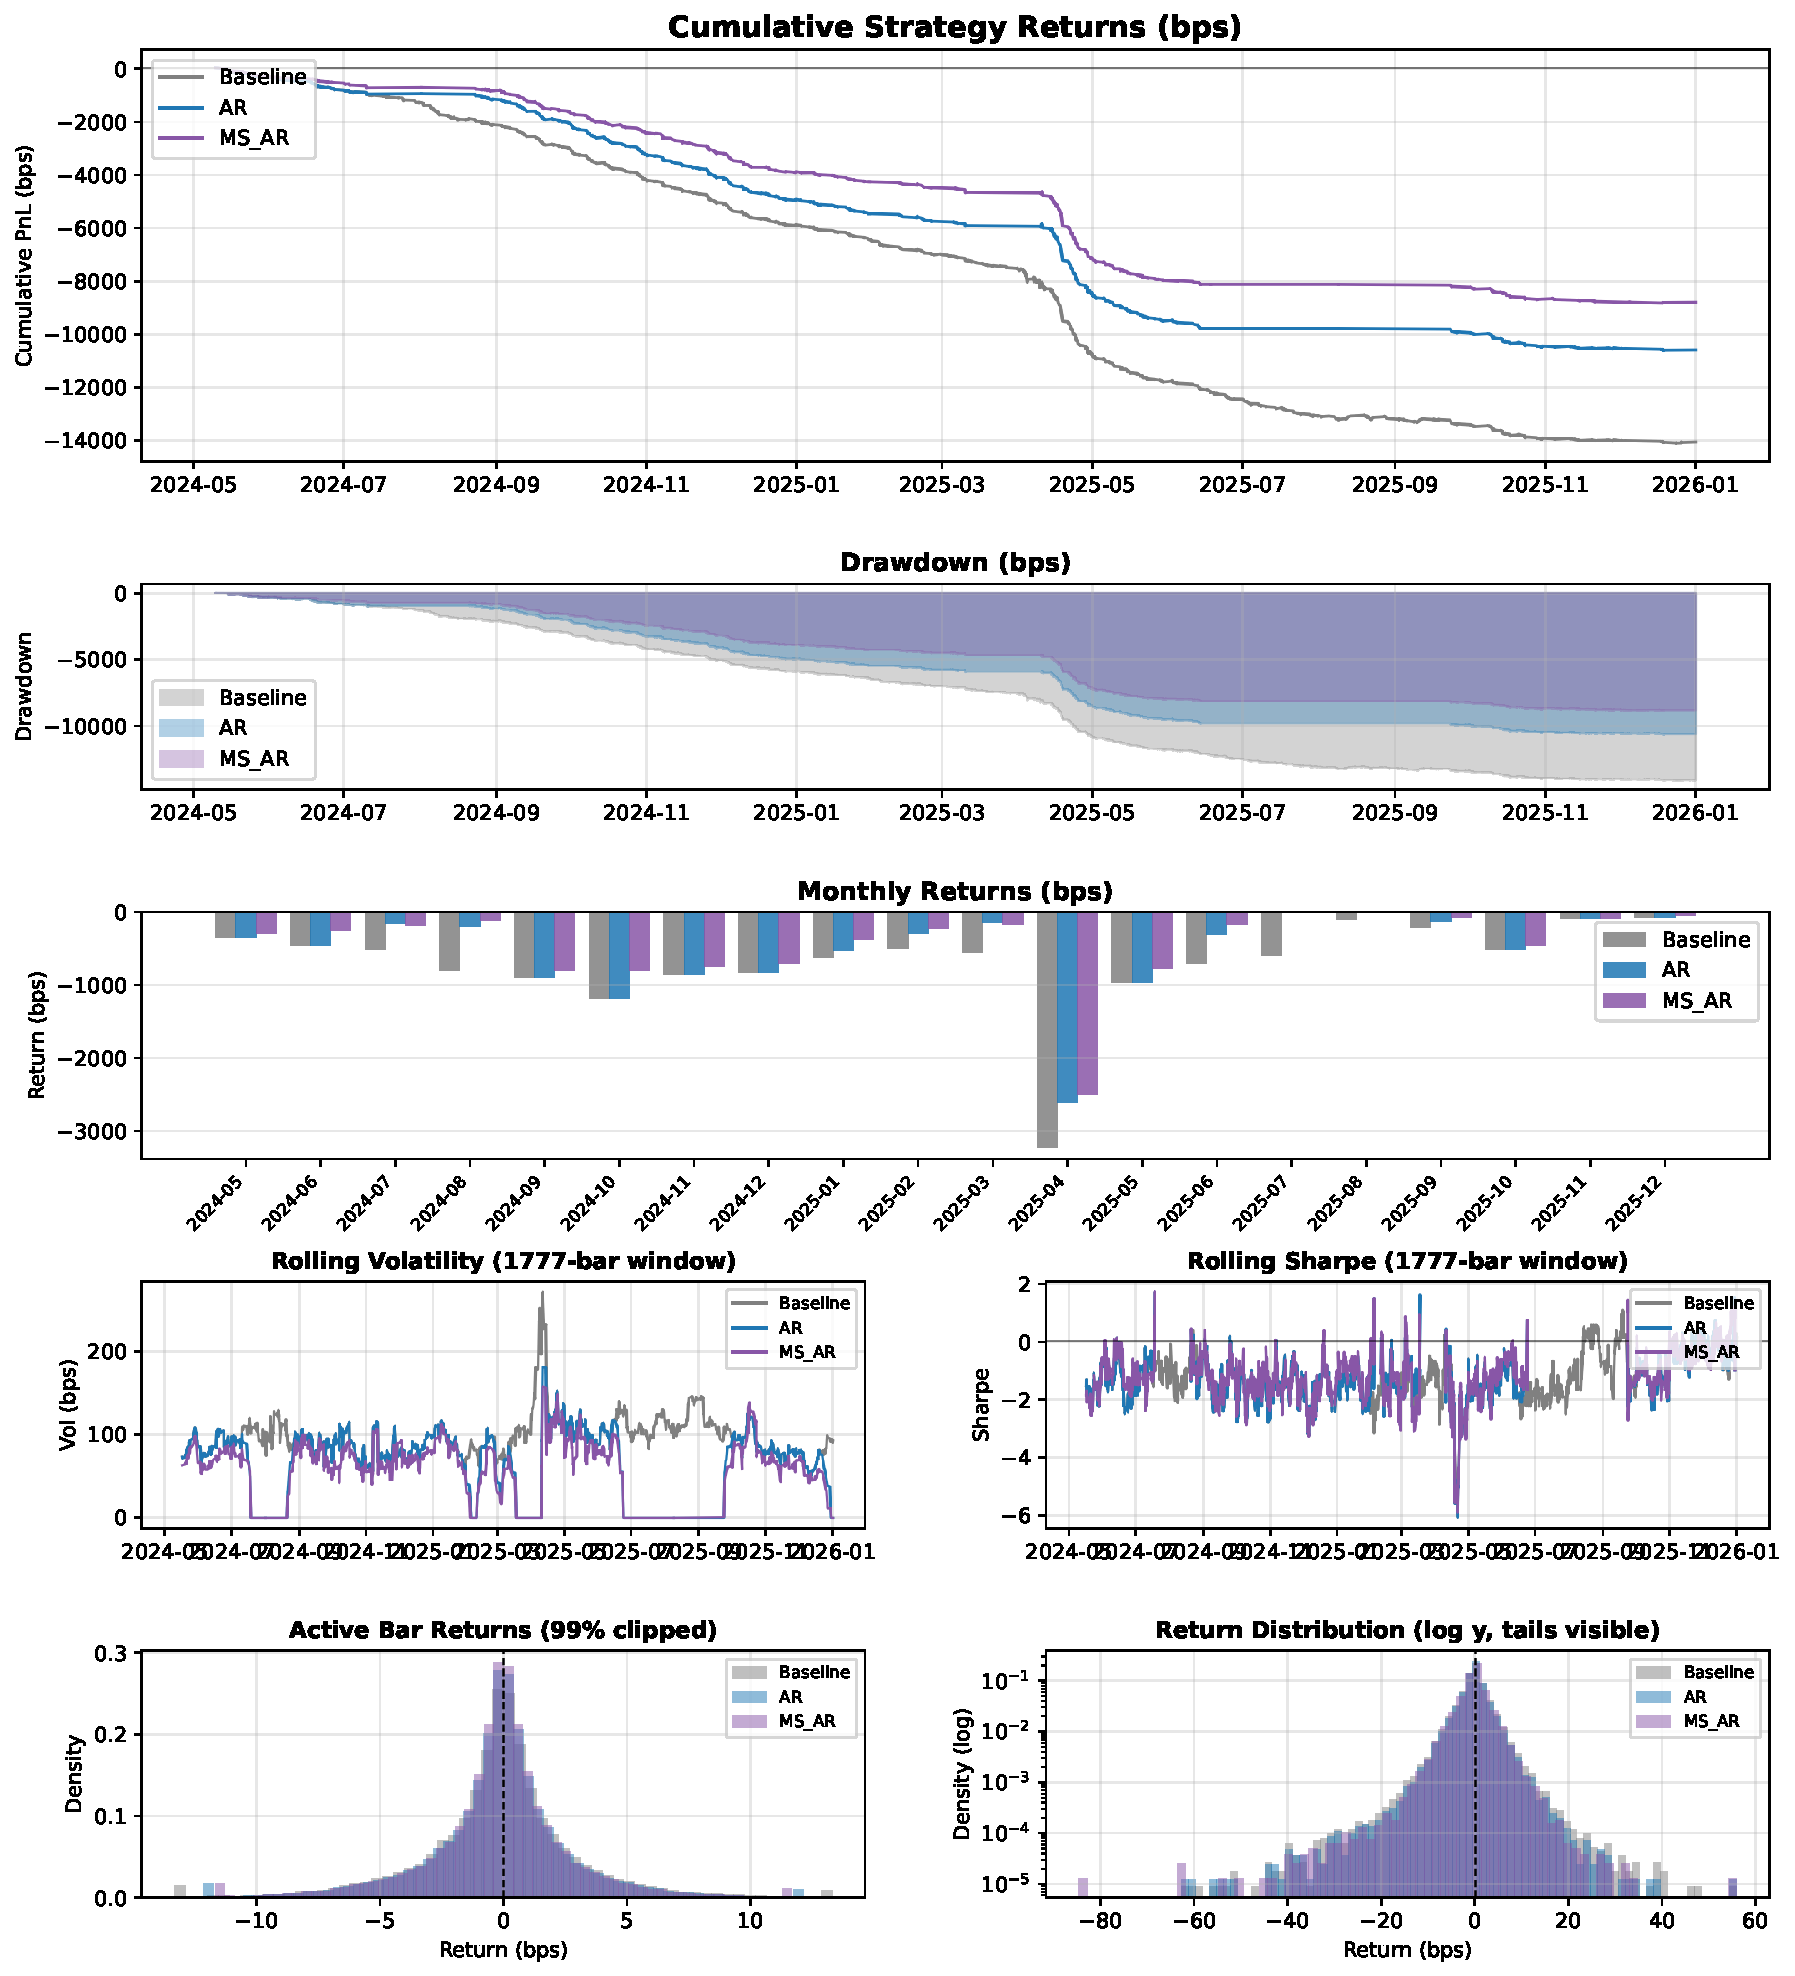
\includegraphics[width=\textwidth]{plots/EURNOK_EURSEK_performance.pdf}
    \caption{Backtest performance for EURNOK/EURSEK across the baseline, AR, and Markov-switching AR strategies. The figure compares cumulative returns, drawdowns, monthly return contributions, rolling volatility, rolling Sharpe ratios, active-bar return densities, and tail behaviour.}
    \label{fig:EURNOK_EURSEK_performance}
\end{figure}

\subsubsection{GBPUSD/EURUSD}

\begin{figure}[H]
    \centering
    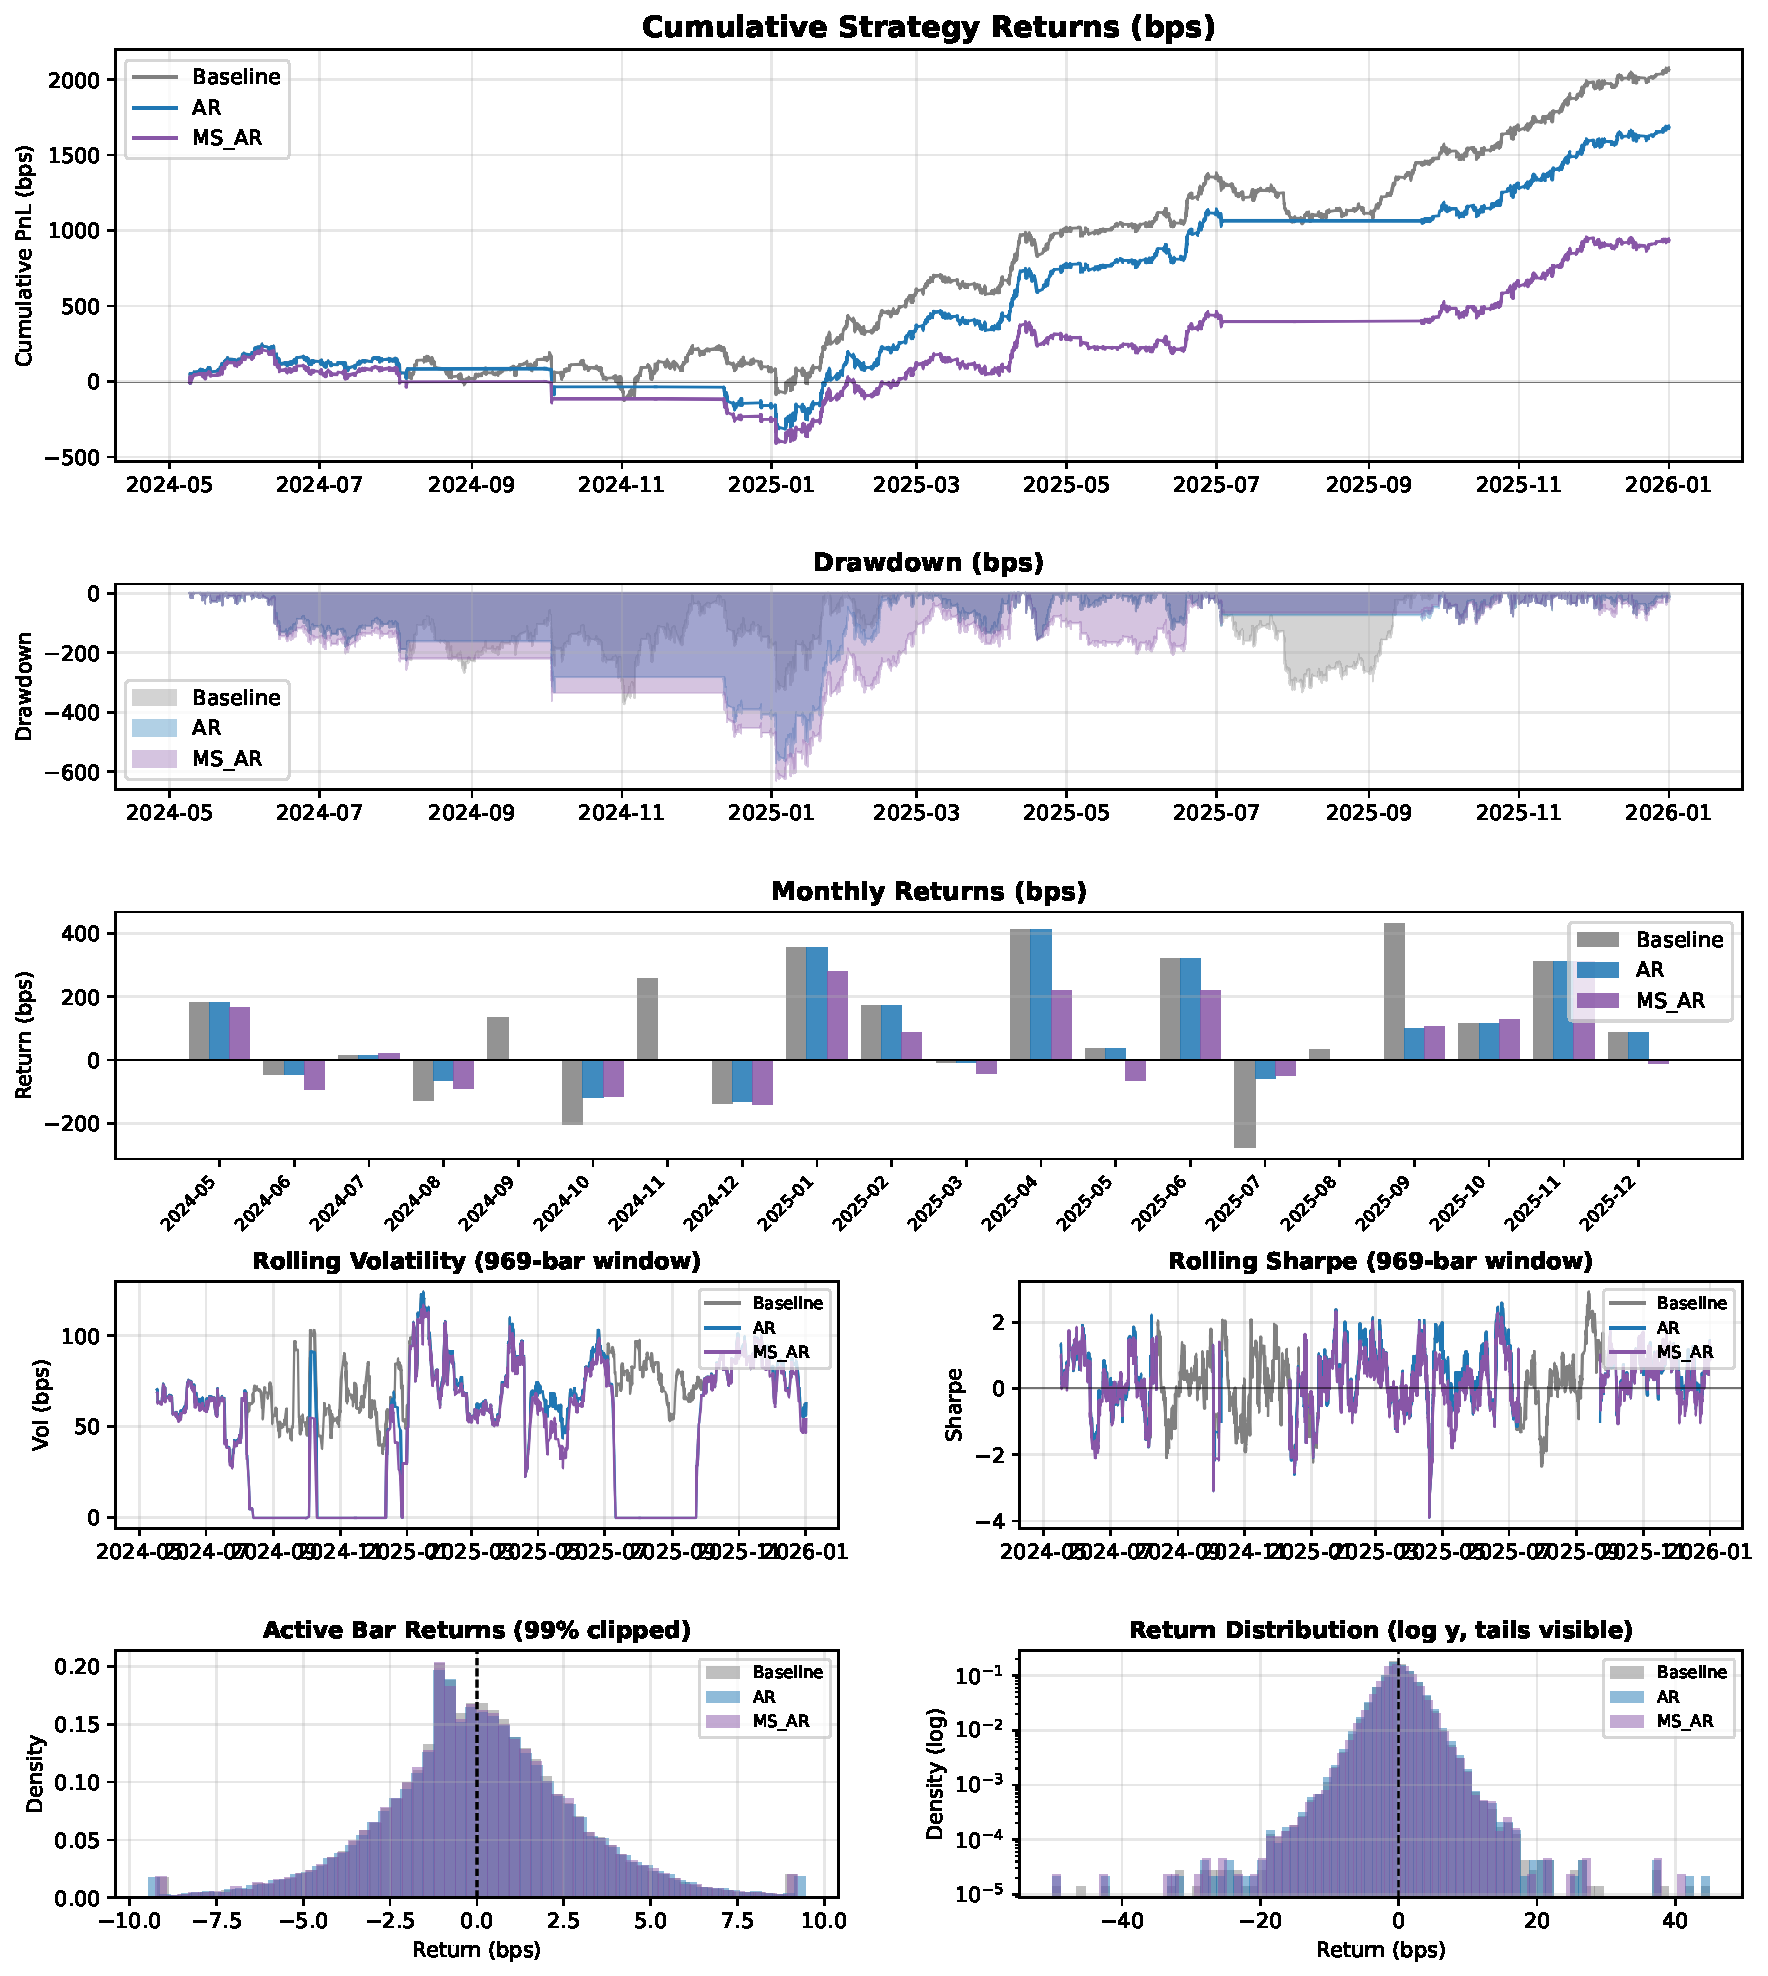
\includegraphics[width=\textwidth]{plots/GBPUSD_EURUSD_performance.pdf}
    \caption{Backtest performance for GBPUSD/EURUSD across the baseline, AR, and Markov-switching AR strategies. The figure compares cumulative returns, drawdowns, monthly returns, rolling volatility, rolling Sharpe ratios, active-bar return densities, and tail behaviour under the competing model specifications.}
    \label{fig:GBPUSD_EURUSD_performance}
\end{figure}


%%%%%%%%%%%%%%%%%%%%%%%%%%%%%%%%%%%%%%%%%%%%%%%%%%%%%%%%%%%%%%
%%%%%%%%%%%%%%%%%%%%%%%%%%%%%%%%%%%%%%%%%%%%%%%%%%%%%%%%%%%%%%
%%%%%%%%%%%%%%%%%%%%%%%%%%%%%%%%%%%%%%%%%%%%%%%%%%%%%%%%%%%%%%

\subsection{Currency pair tables -- rolling}

\begin{table}[H]
\centering
\caption{Rolling strategy tearsheets across all currency pairs. Returns, volatility, drawdowns, VaR, CVaR, average wins, and losses are reported in basis points.}
\label{tab:rolling_strategy_tearsheets_all_pairs}
\small
\setlength{\tabcolsep}{2.0pt}
\renewcommand{\arraystretch}{2.5}

\begin{adjustbox}{max width=\linewidth, max totalheight=0.90\textheight}
\begin{tabular}{lrrrrrrrrrrrr}
\toprule
& \multicolumn{4}{c}{\textbf{AUDUSD/NZDUSD}}
& \multicolumn{4}{c}{\textbf{EURNOK/EURSEK}}
& \multicolumn{4}{c}{\textbf{GBPUSD/EURUSD}} \\
\cmidrule(lr){2-5}
\cmidrule(lr){6-9}
\cmidrule(lr){10-13}
\textbf{Metric}
& \textbf{BH} & \textbf{Base} & \textbf{AR} & \textbf{MS-AR}
& \textbf{BH} & \textbf{Base} & \textbf{AR} & \textbf{MS-AR}
& \textbf{BH} & \textbf{Base} & \textbf{AR} & \textbf{MS-AR} \\
\midrule
Total return              & 326.82 & 5339.28 & 2684.12 & -738.81 & 1568.39 & -1732.23 & -1202.96 & -22954.49 & 415.21 & 3318.37 & 1551.09 & -1852.92 \\
Annual return             & 198.95 & 3250.29 & 1633.96 & -449.75 & 954.76 & -1054.49 & -732.30 & -13973.54 & 252.76 & 2020.06 & 944.23 & -1127.96 \\
Best month                & 276.13 & 922.91 & 828.76 & 199.96 & 385.45 & 130.57 & 158.91 & -213.68 & 227.80 & 418.93 & 263.57 & 85.13 \\
Worst month               & -175.00 & -129.96 & -101.70 & -226.18 & -226.61 & -372.48 & -350.24 & -3985.96 & -208.05 & -123.05 & -194.75 & -519.47 \\
Positive months           & 65.00\% & 95.00\% & 90.00\% & 40.00\% & 70.00\% & 30.00\% & 40.00\% & 0.00\% & 50.00\% & 80.00\% & 80.00\% & 25.00\% \\
Annual volatility         & 1023.51 & 614.34 & 467.56 & 385.30 & 999.94 & 632.40 & 571.47 & 517.01 & 805.10 & 561.13 & 459.94 & 338.58 \\
Max drawdown              & -504.21 & -306.40 & -233.48 & -1176.73 & -972.51 & -2082.62 & -1582.85 & -22964.22 & -631.62 & -215.74 & -328.07 & -2015.86 \\
Max drawdown duration     & 10170 & 3779 & 4333 & 14095 & 25593 & 63985 & 63985 & 64222 & 11943 & 3916 & 8878 & 35398 \\
Ulcer index               & 254.32 & 57.55 & 48.38 & 472.63 & 346.12 & 1238.28 & 972.12 & 13057.12 & 248.38 & 67.83 & 100.58 & 1056.65 \\
VaR 95\%                  & -12.50 & -6.73 & -3.86 & -3.42 & -7.34 & -3.74 & -3.07 & -3.77 & -7.96 & -5.53 & -4.34 & -2.82 \\
CVaR 95\%                 & -17.86 & -11.37 & -8.72 & -7.07 & -12.07 & -8.21 & -7.41 & -7.82 & -11.50 & -8.82 & -7.56 & -5.40 \\
Sharpe ratio              & 0.19 & 5.29 & 3.49 & -1.17 & 0.95 & -1.67 & -1.28 & -27.03 & 0.31 & 3.60 & 2.05 & -3.33 \\
Sortino ratio             & 0.28 & 5.29 & 2.65 & -1.09 & 1.22 & -1.13 & -0.81 & -17.67 & 0.46 & 3.83 & 1.76 & -3.18 \\
Calmar ratio              & 0.39 & 10.61 & 7.00 & 0.38 & 0.98 & 0.51 & 0.46 & 0.61 & 0.40 & 9.36 & 2.88 & 0.56 \\
Profit factor             & 1.00 & 1.21 & 1.19 & 0.95 & 1.02 & 0.95 & 0.96 & 0.39 & 1.01 & 1.10 & 1.07 & 0.90 \\
Payoff ratio              & 1.00 & 1.21 & 1.22 & 1.48 & 1.01 & 1.00 & 1.00 & 1.02 & 1.01 & 1.12 & 1.11 & 1.20 \\
Tail ratio                & 1.00 & 1.20 & 1.24 & 0.96 & 1.03 & 0.97 & 0.96 & 0.20 & 1.01 & 1.08 & 1.03 & 0.93 \\
Number of trades          & 0 & 570 & 302 & 4542 & 0 & 700 & 580 & 8612 & 0 & 994 & 547 & 9235 \\
Win rate                  & 50.21\% & 50.04\% & 49.39\% & 39.08\% & 50.06\% & 48.80\% & 49.05\% & 27.95\% & 49.87\% & 49.42\% & 49.15\% & 42.85\% \\
Market exposure           & 99.92\% & 36.06\% & 20.34\% & 34.62\% & 99.95\% & 27.19\% & 22.57\% & 26.92\% & 99.89\% & 49.80\% & 31.66\% & 48.07\% \\
Average win               & 5.84 & 6.31 & 6.33 & 3.67 & 3.13 & 3.93 & 3.96 & 3.08 & 3.76 & 3.90 & 3.97 & 2.02 \\
Average loss              & -5.87 & -5.21 & -5.19 & -2.48 & -3.09 & -3.94 & -3.98 & -3.04 & -3.72 & -3.46 & -3.59 & -1.69 \\
Skewness                  & -0.06 & 1.68 & 2.81 & 4.47 & 0.09 & -0.12 & 0.04 & -2.16 & 0.74 & 0.92 & 1.46 & 2.62 \\
Kurtosis                  & 7.52 & 27.84 & 62.92 & 109.50 & 19.12 & 57.67 & 57.84 & 66.08 & 34.61 & 28.55 & 55.78 & 129.83 \\
\bottomrule
\end{tabular}
\end{adjustbox}

\end{table}

%%%%%%%%%%%%%%%%%%%%%%%%%%%%%%%%%%%%%%%%%%%%%%%%%%%%%%%%%%%%%%
%%%%%%%%%%%%%%%%%%%%%%%%%%%%%%%%%%%%%%%%%%%%%%%%%%%%%%%%%%%%%%
%%%%%%%%%%%%%%%%%%%%%%%%%%%%%%%%%%%%%%%%%%%%%%%%%%%%%%%%%%%%%%

\clearpage\subsection{Currency pair tables -- independent days}

\begin{table}[H]
\centering
\caption{Daily strategy tearsheets across all currency pairs. Returns, volatility, drawdowns, VaR, CVaR, average wins, and losses are reported in basis points.}
\label{tab:daily_strategy_tearsheets_all_pairs}
\small
\setlength{\tabcolsep}{2.0pt}
\renewcommand{\arraystretch}{2.5}

\begin{adjustbox}{max width=\linewidth, max totalheight=0.90\textheight}
\begin{tabular}{lrrrrrrrrrrrr}
\toprule
& \multicolumn{4}{c}{\textbf{AUDUSD/NZDUSD}}
& \multicolumn{4}{c}{\textbf{EURNOK/EURSEK}}
& \multicolumn{4}{c}{\textbf{GBPUSD/EURUSD}} \\
\cmidrule(lr){2-5}
\cmidrule(lr){6-9}
\cmidrule(lr){10-13}
\textbf{Metric}
& \textbf{BH} & \textbf{Base} & \textbf{AR} & \textbf{MS-AR}
& \textbf{BH} & \textbf{Base} & \textbf{AR} & \textbf{MS-AR}
& \textbf{BH} & \textbf{Base} & \textbf{AR} & \textbf{MS-AR} \\
\midrule
Total return              & 326.82 & 6752.23 & 3543.86 & -876.77 & 1568.39 & -2458.13 & -1865.68 & -21067.82 & 415.21 & 2623.58 & 979.72 & -1880.54 \\
Annual return             & 198.95 & 4110.42 & 2157.33 & -533.73 & 954.76 & -1496.39 & -1135.73 & -12825.04 & 252.76 & 1597.10 & 596.40 & -1144.78 \\
Best month                & 276.13 & 881.06 & 723.66 & 218.43 & 385.45 & 85.83 & 109.03 & -160.47 & 227.80 & 421.07 & 283.67 & 77.58 \\
Worst month               & -175.00 & -195.89 & -42.17 & -329.10 & -226.61 & -403.50 & -389.74 & -3741.58 & -208.05 & -218.37 & -125.87 & -507.80 \\
Positive months           & 65.00\% & 85.00\% & 85.00\% & 45.00\% & 70.00\% & 25.00\% & 35.00\% & 0.00\% & 50.00\% & 80.00\% & 70.00\% & 30.00\% \\
Annual volatility         & 1023.51 & 657.14 & 488.91 & 417.60 & 999.94 & 626.54 & 553.41 & 508.70 & 805.10 & 535.11 & 437.33 & 327.79 \\
Max drawdown              & -504.21 & -364.82 & -194.67 & -1072.22 & -972.51 & -2740.28 & -2171.77 & -21077.55 & -631.62 & -254.82 & -261.81 & -2080.09 \\
Max drawdown duration     & 10170 & 3738 & 3625 & 14303 & 25593 & 63985 & 63985 & 64222 & 11943 & 3875 & 10970 & 35398 \\
Ulcer index               & 254.32 & 84.53 & 53.11 & 534.36 & 346.12 & 1635.93 & 1310.10 & 12015.99 & 248.38 & 74.10 & 89.82 & 1128.74 \\
VaR 95\%                  & -12.50 & -7.36 & -4.37 & -4.05 & -7.34 & -3.66 & -2.75 & -3.58 & -7.96 & -5.23 & -3.89 & -2.65 \\
CVaR 95\%                 & -17.86 & -11.86 & -8.98 & -7.66 & -12.07 & -8.21 & -7.19 & -7.67 & -11.50 & -8.54 & -7.25 & -5.25 \\
Sharpe ratio              & 0.19 & 6.26 & 4.41 & -1.28 & 0.95 & -2.39 & -2.05 & -25.21 & 0.31 & 2.98 & 1.36 & -3.49 \\
Sortino ratio             & 0.28 & 6.90 & 3.62 & -1.29 & 1.22 & -1.56 & -1.21 & -15.80 & 0.46 & 2.98 & 1.08 & -3.13 \\
Calmar ratio              & 0.39 & 11.27 & 11.08 & 0.50 & 0.98 & 0.55 & 0.52 & 0.61 & 0.40 & 6.27 & 2.28 & 0.55 \\
Profit factor             & 1.00 & 1.23 & 1.22 & 0.95 & 1.02 & 0.93 & 0.93 & 0.41 & 1.01 & 1.09 & 1.05 & 0.89 \\
Payoff ratio              & 1.00 & 1.26 & 1.27 & 1.46 & 1.01 & 0.99 & 0.98 & 1.03 & 1.01 & 1.13 & 1.11 & 1.19 \\
Tail ratio                & 1.00 & 1.23 & 1.26 & 1.02 & 1.03 & 0.94 & 0.88 & 0.17 & 1.01 & 1.07 & 1.04 & 0.91 \\
Number of trades          & 0 & 1048 & 550 & 5625 & 0 & 718 & 576 & 7897 & 0 & 910 & 494 & 8130 \\
Win rate                  & 50.21\% & 49.31\% & 49.17\% & 39.31\% & 50.06\% & 48.37\% & 48.60\% & 28.33\% & 49.87\% & 49.06\% & 48.61\% & 42.59\% \\
Market exposure           & 99.92\% & 44.14\% & 23.88\% & 42.61\% & 99.95\% & 24.95\% & 19.67\% & 24.69\% & 99.89\% & 43.77\% & 26.81\% & 42.37\% \\
Average win               & 5.84 & 6.25 & 6.22 & 3.64 & 3.13 & 4.10 & 4.12 & 3.20 & 3.76 & 3.96 & 4.10 & 2.08 \\
Average loss              & -5.87 & -4.94 & -4.91 & -2.49 & -3.09 & -4.14 & -4.18 & -3.12 & -3.72 & -3.51 & -3.69 & -1.74 \\
Skewness                  & -0.06 & 1.28 & 2.37 & 3.21 & 0.09 & -0.19 & -0.01 & -2.25 & 0.74 & 1.04 & 1.77 & 2.85 \\
Kurtosis                  & 7.52 & 21.37 & 55.48 & 86.15 & 19.12 & 59.86 & 64.57 & 70.27 & 34.61 & 33.65 & 72.02 & 147.66 \\
\bottomrule
\end{tabular}
\end{adjustbox}

\end{table}

%%%%%%%%%%%%%%%%%%%%%%%%%%%%%%%%%%%%%%%%%%%%%%%%%%%%%%%%%%%%%%
%%%%%%%%%%%%%%%%%%%%%%%%%%%%%%%%%%%%%%%%%%%%%%%%%%%%%%%%%%%%%%
%%%%%%%%%%%%%%%%%%%%%%%%%%%%%%%%%%%%%%%%%%%%%%%%%%%%%%%%%%%%%%

\subsection{Markov Dynamics}

\subsubsection{AUDUSD/NZDUSD}

\begin{figure}[H]
    \centering
    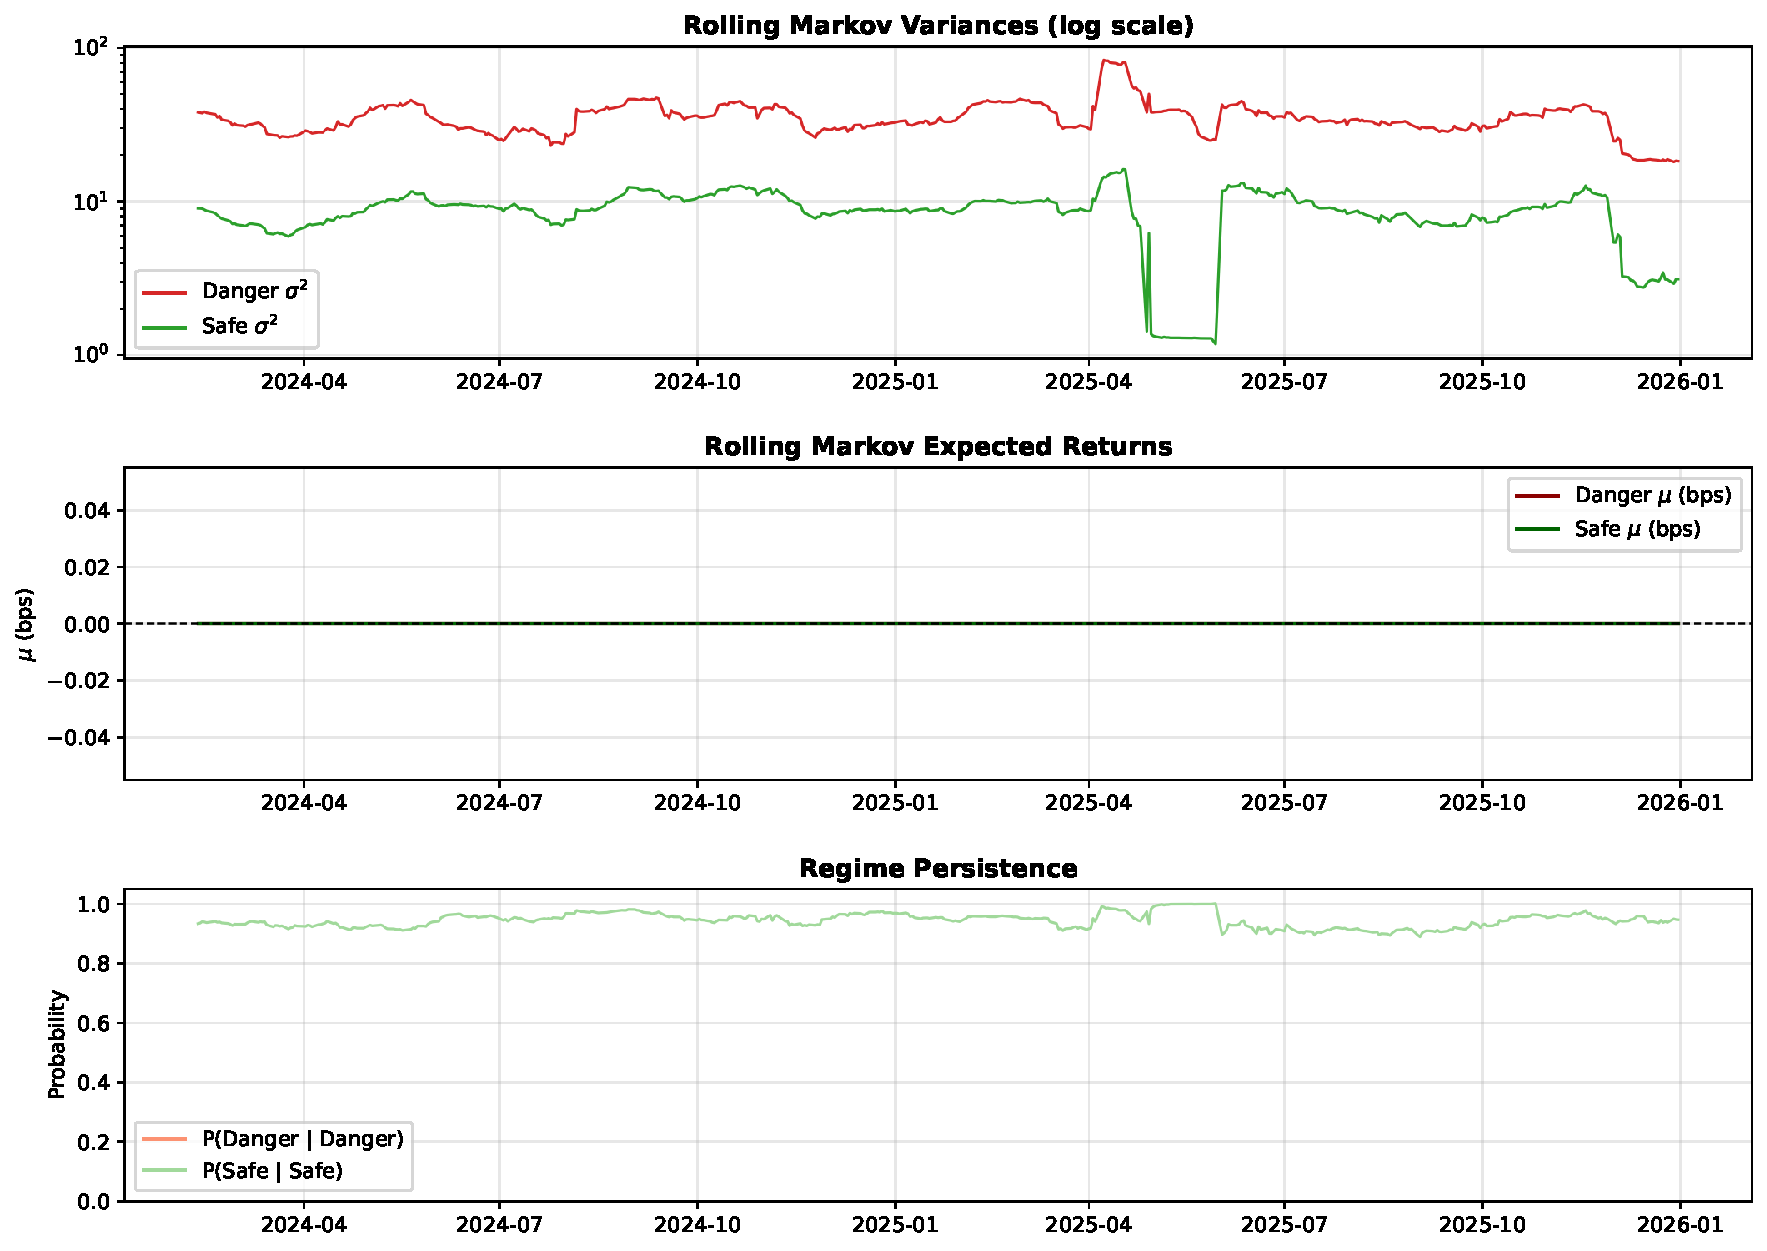
\includegraphics[width=\textwidth]{plots/AUDUSD_NZDUSD_markov_dynamics.pdf}
    \caption{Estimated Markov-regime dynamics for AUDUSD/NZDUSD. The figure reports rolling estimates of regime-specific variance, expected return, and regime persistence, illustrating how the hidden Markov structure classifies changing market conditions through time.}
    \label{fig:AUDUSD_NZDUSD_markov_dynamics}
\end{figure}

\subsubsection{EURNOK/EURSEK}

\begin{figure}[H]
    \centering
    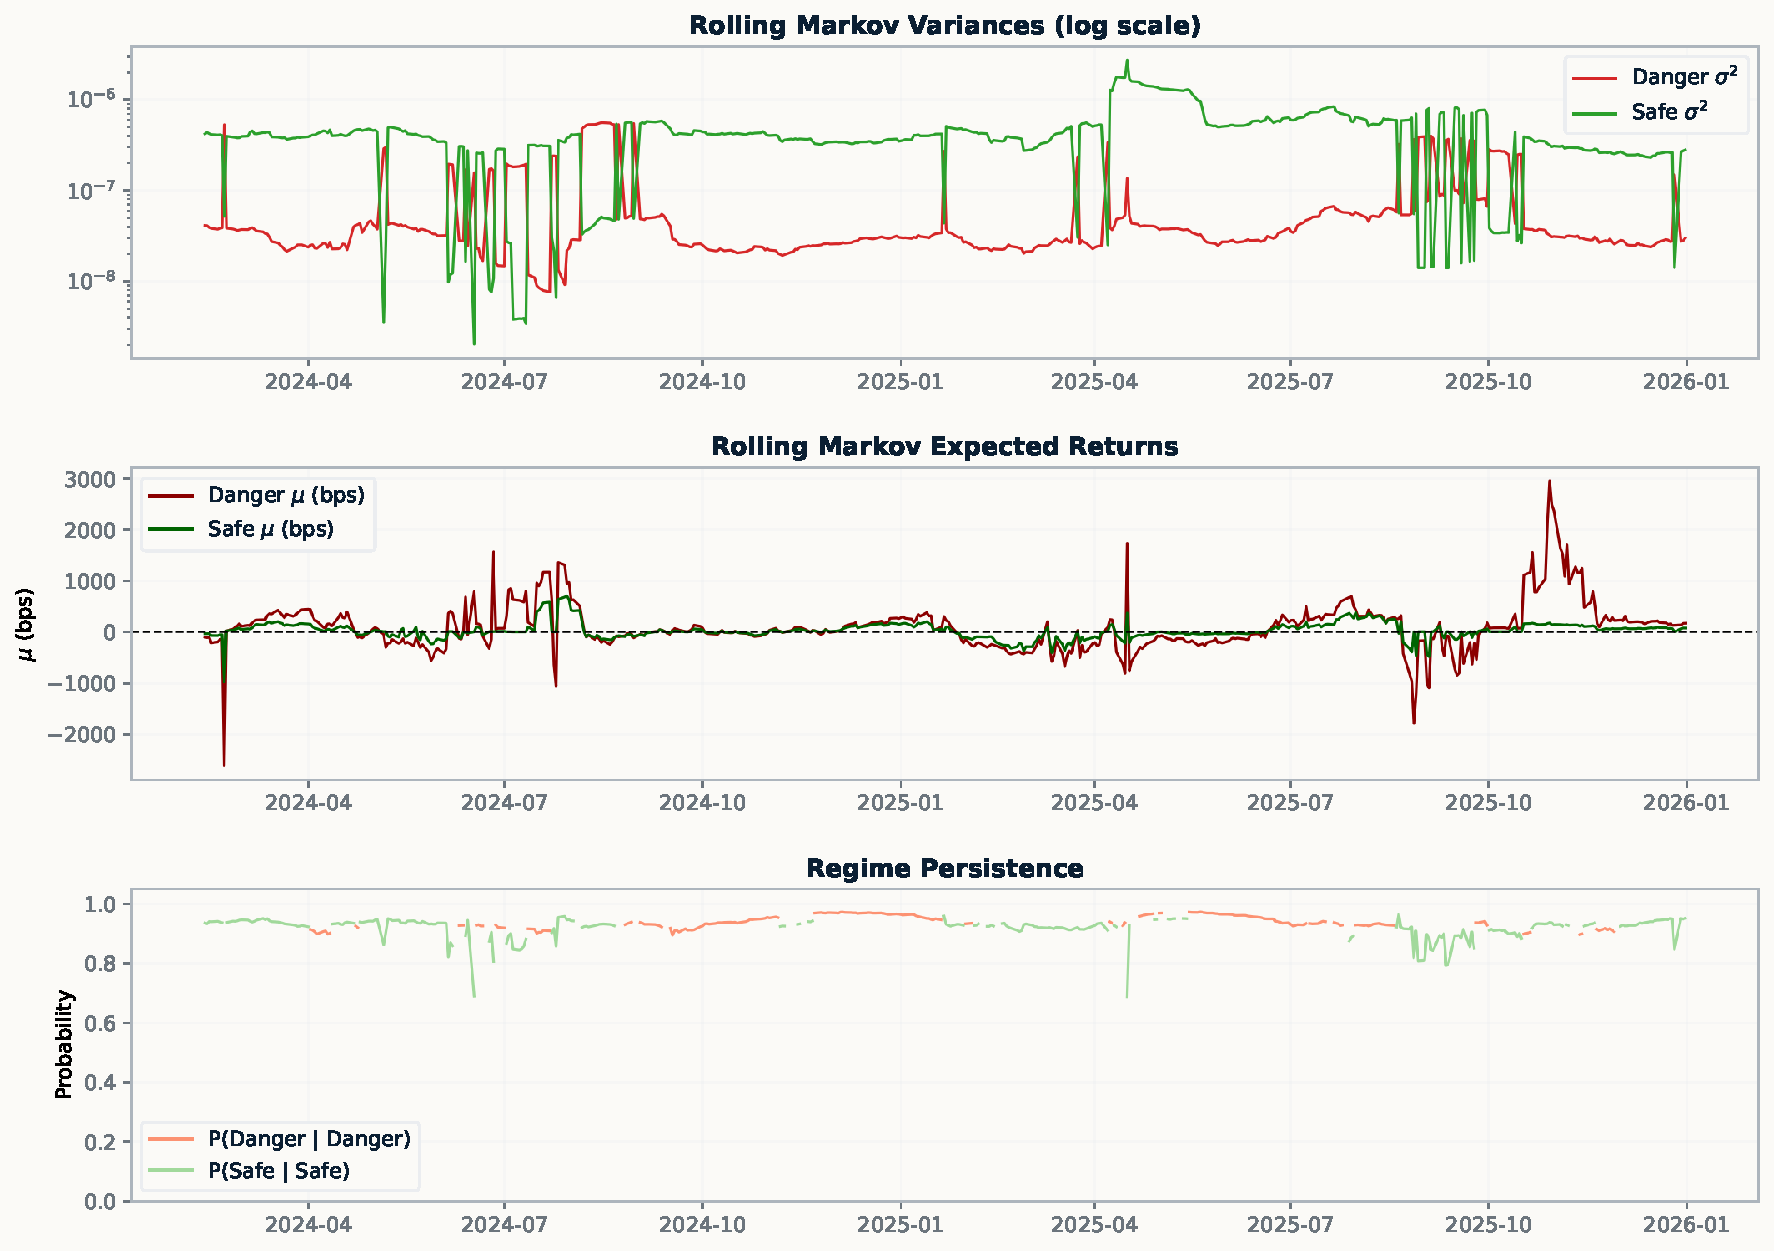
\includegraphics[width=\textwidth]{plots/EURNOK_EURSEK_markov_dynamics.pdf}
    \caption{Estimated Markov-regime dynamics for EURNOK/EURSEK. The figure reports rolling estimates of regime-specific variance, expected return, and regime persistence, illustrating how the hidden Markov structure classifies changing market conditions through time.}
    \label{fig:EURNOK_EURSEK_markov_dynamics}
\end{figure}

\subsubsection{GBPUSD/EURUSD}

\begin{figure}[H]
    \centering
    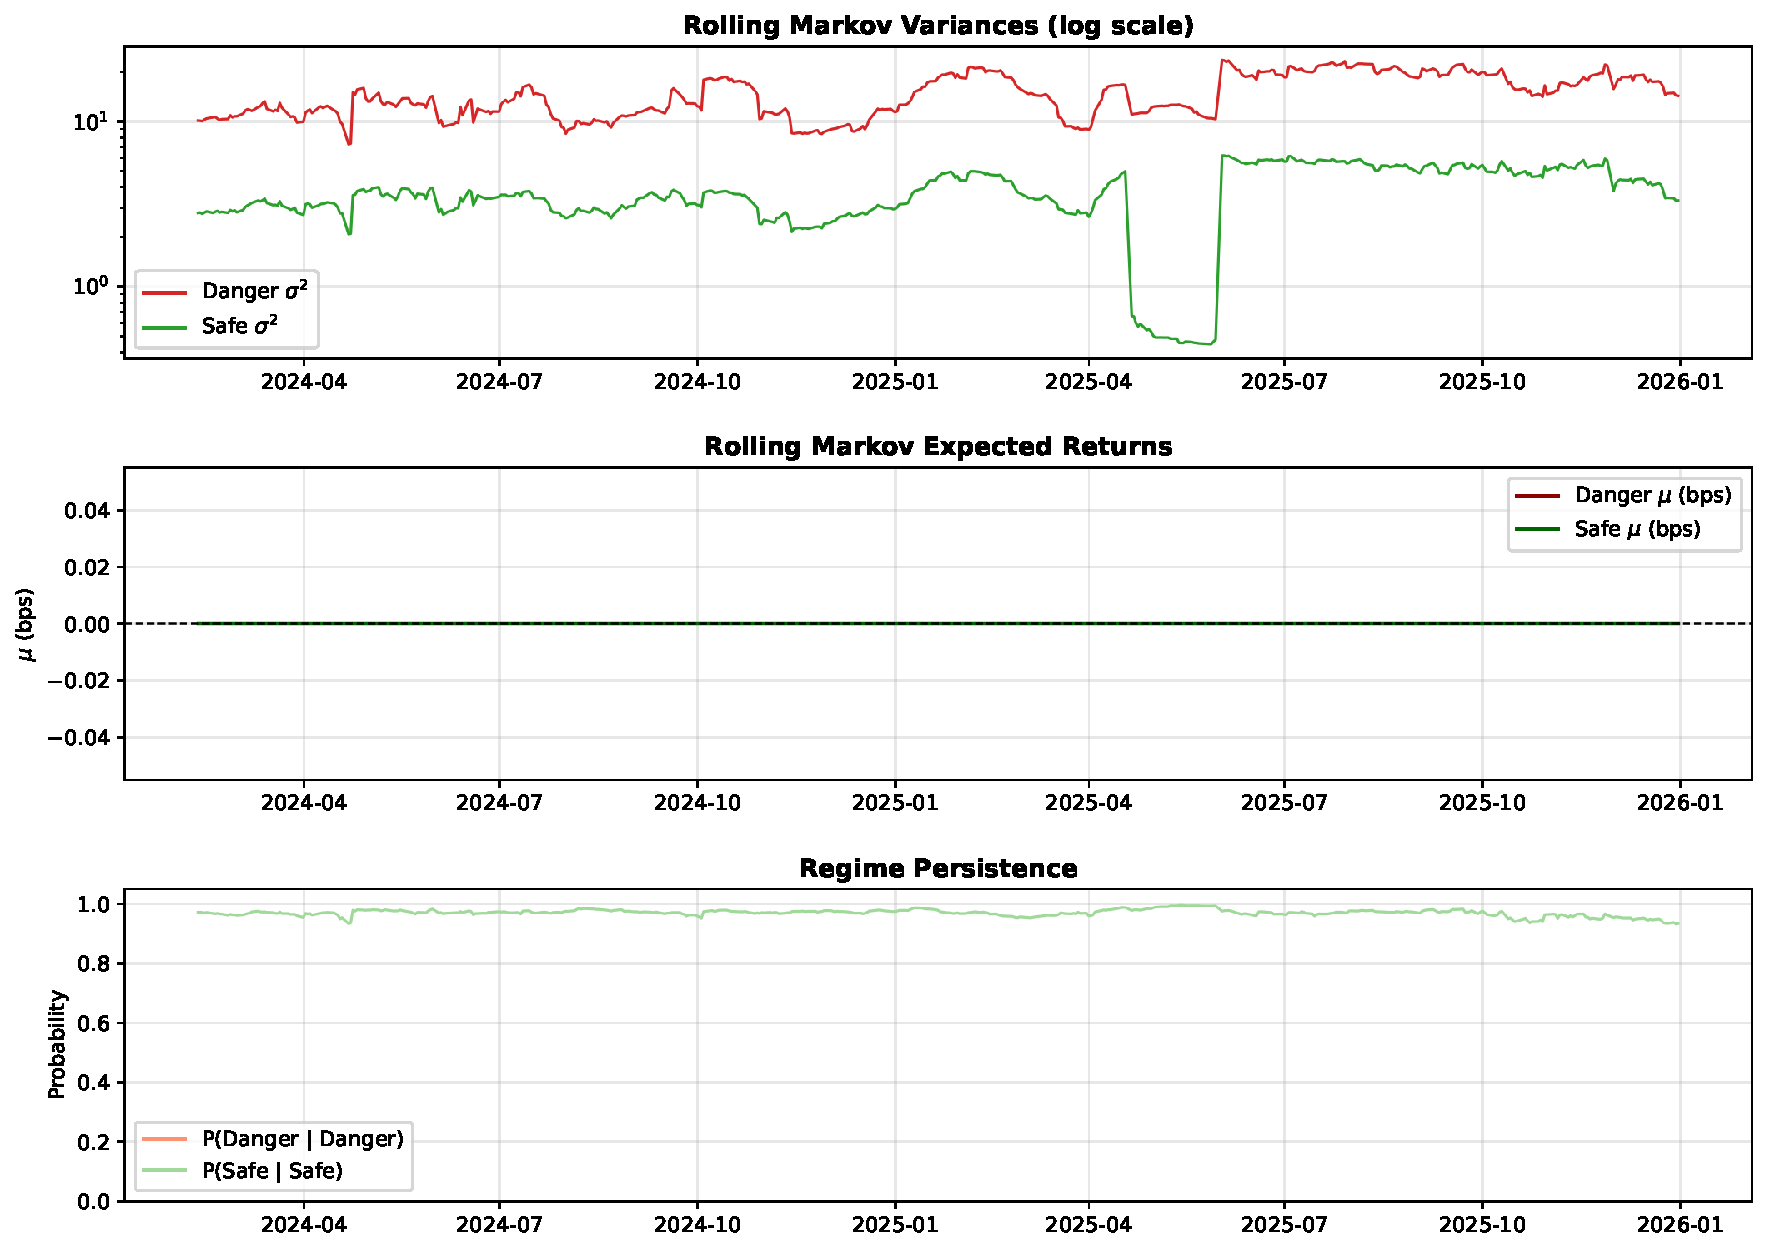
\includegraphics[width=\textwidth]{plots/GBPUSD_EURUSD_markov_dynamics.pdf}
    \caption{Estimated Markov-regime dynamics for GBPUSD/EURUSD. The figure reports rolling estimates of regime-specific variance, expected return, and regime persistence, illustrating how the hidden Markov structure classifies changing market conditions through time.}
    \label{fig:GBPUSD_EURUSD_markov_dynamics}
\end{figure}

%%%%%%%%%%%%%%%%%%%%%%%%%%%%%%%%%%%%%%%%%%%%%%%%%%%%%%%%%%%%%%
%%%%%%%%%%%%%%%%%%%%%%%%%%%%%%%%%%%%%%%%%%%%%%%%%%%%%%%%%%%%%%
%%%%%%%%%%%%%%%%%%%%%%%%%%%%%%%%%%%%%%%%%%%%%%%%%%%%%%%%%%%%%%

\subsection{Positions and regimes}

\subsubsection{AUDUSD/NZDUSD}

\begin{figure}[H]
    \centering
    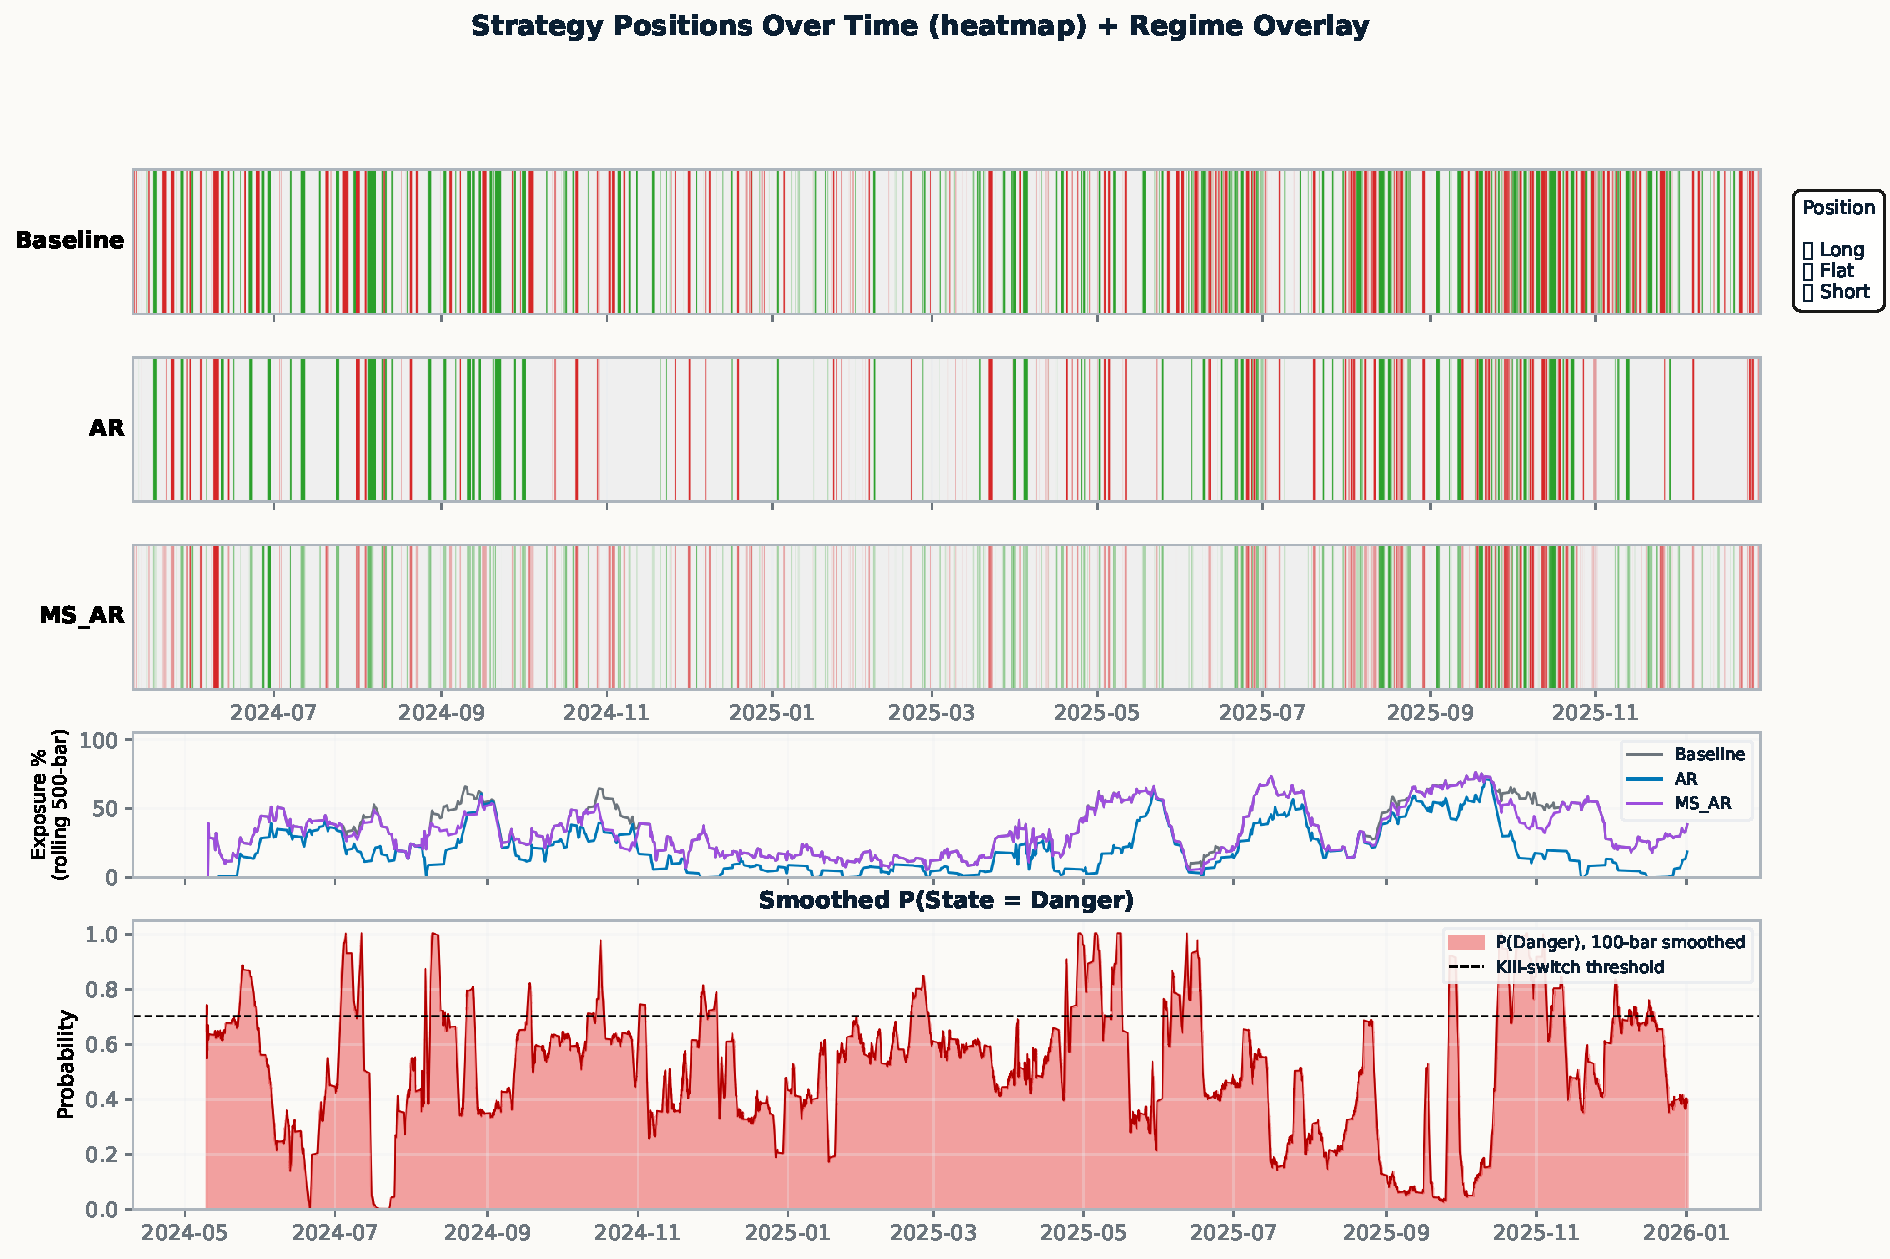
\includegraphics[width=\textwidth]{plots/AUDUSD_NZDUSD_positions_and_regimes.pdf}
    \caption{Trading positions and regime overlays for AUDUSD/NZDUSD. The figure shows exposure across the baseline, AR, and Markov-switching AR strategies, together with the smoothed dangerous-regime probability and the resulting long, flat, and short trading states.}
    \label{fig:AUDUSD_NZDUSD_positions_and_regimes}
\end{figure}

\subsubsection{EURNOK/EURSEK}

\begin{figure}[H]
    \centering
    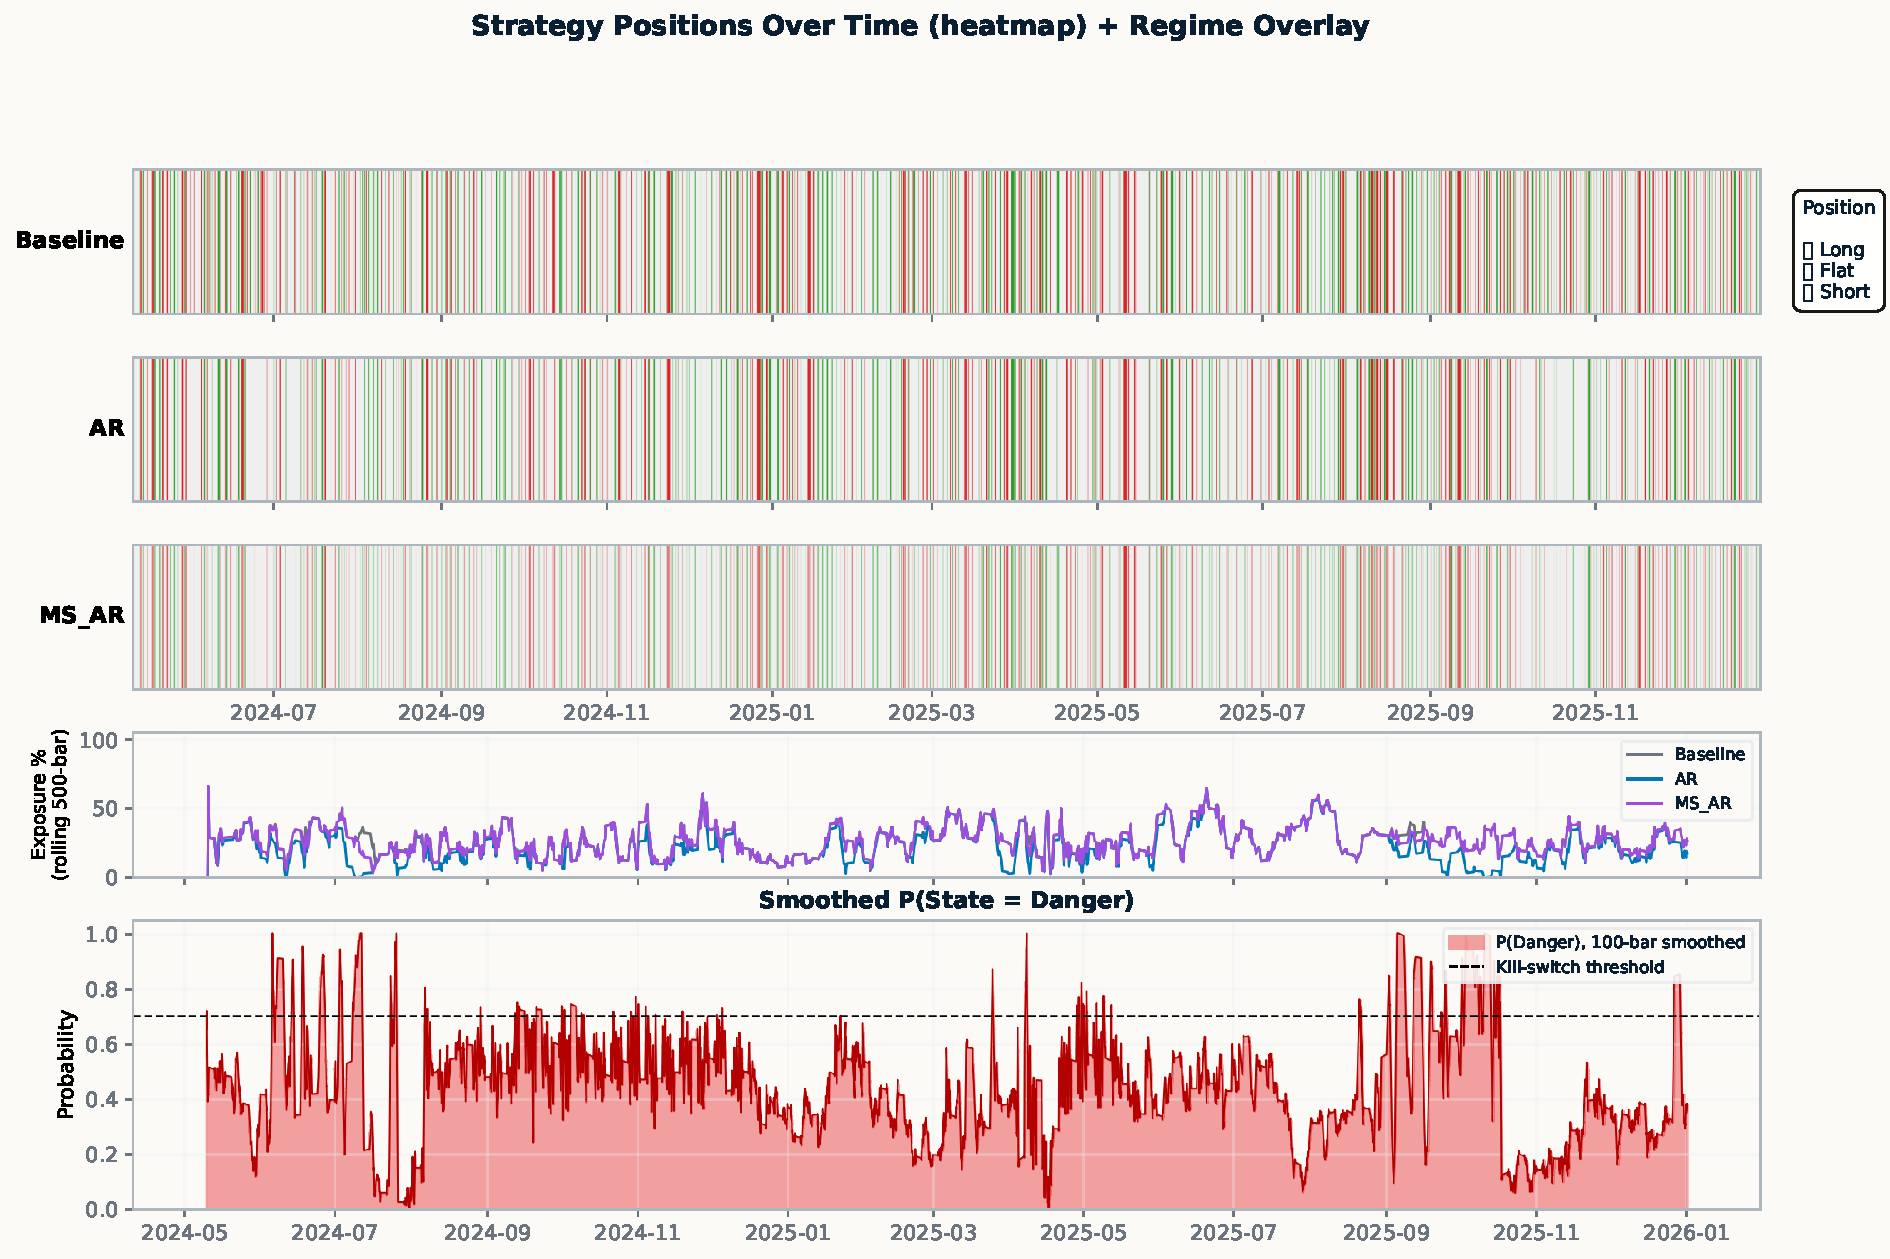
\includegraphics[width=\textwidth]{plots/EURNOK_EURSEK_positions_and_regimes.pdf}
    \caption{Trading positions and regime overlays for EURNOK/EURSEK. The figure shows exposure across the baseline, AR, and Markov-switching AR strategies, together with the smoothed dangerous-regime probability and the resulting long, flat, and short trading states.}
    \label{fig:EURNOK_EURSEK_positions_and_regimes}
\end{figure}

\subsubsection{GBPUSD/EURUSD}

\begin{figure}[H]
    \centering
    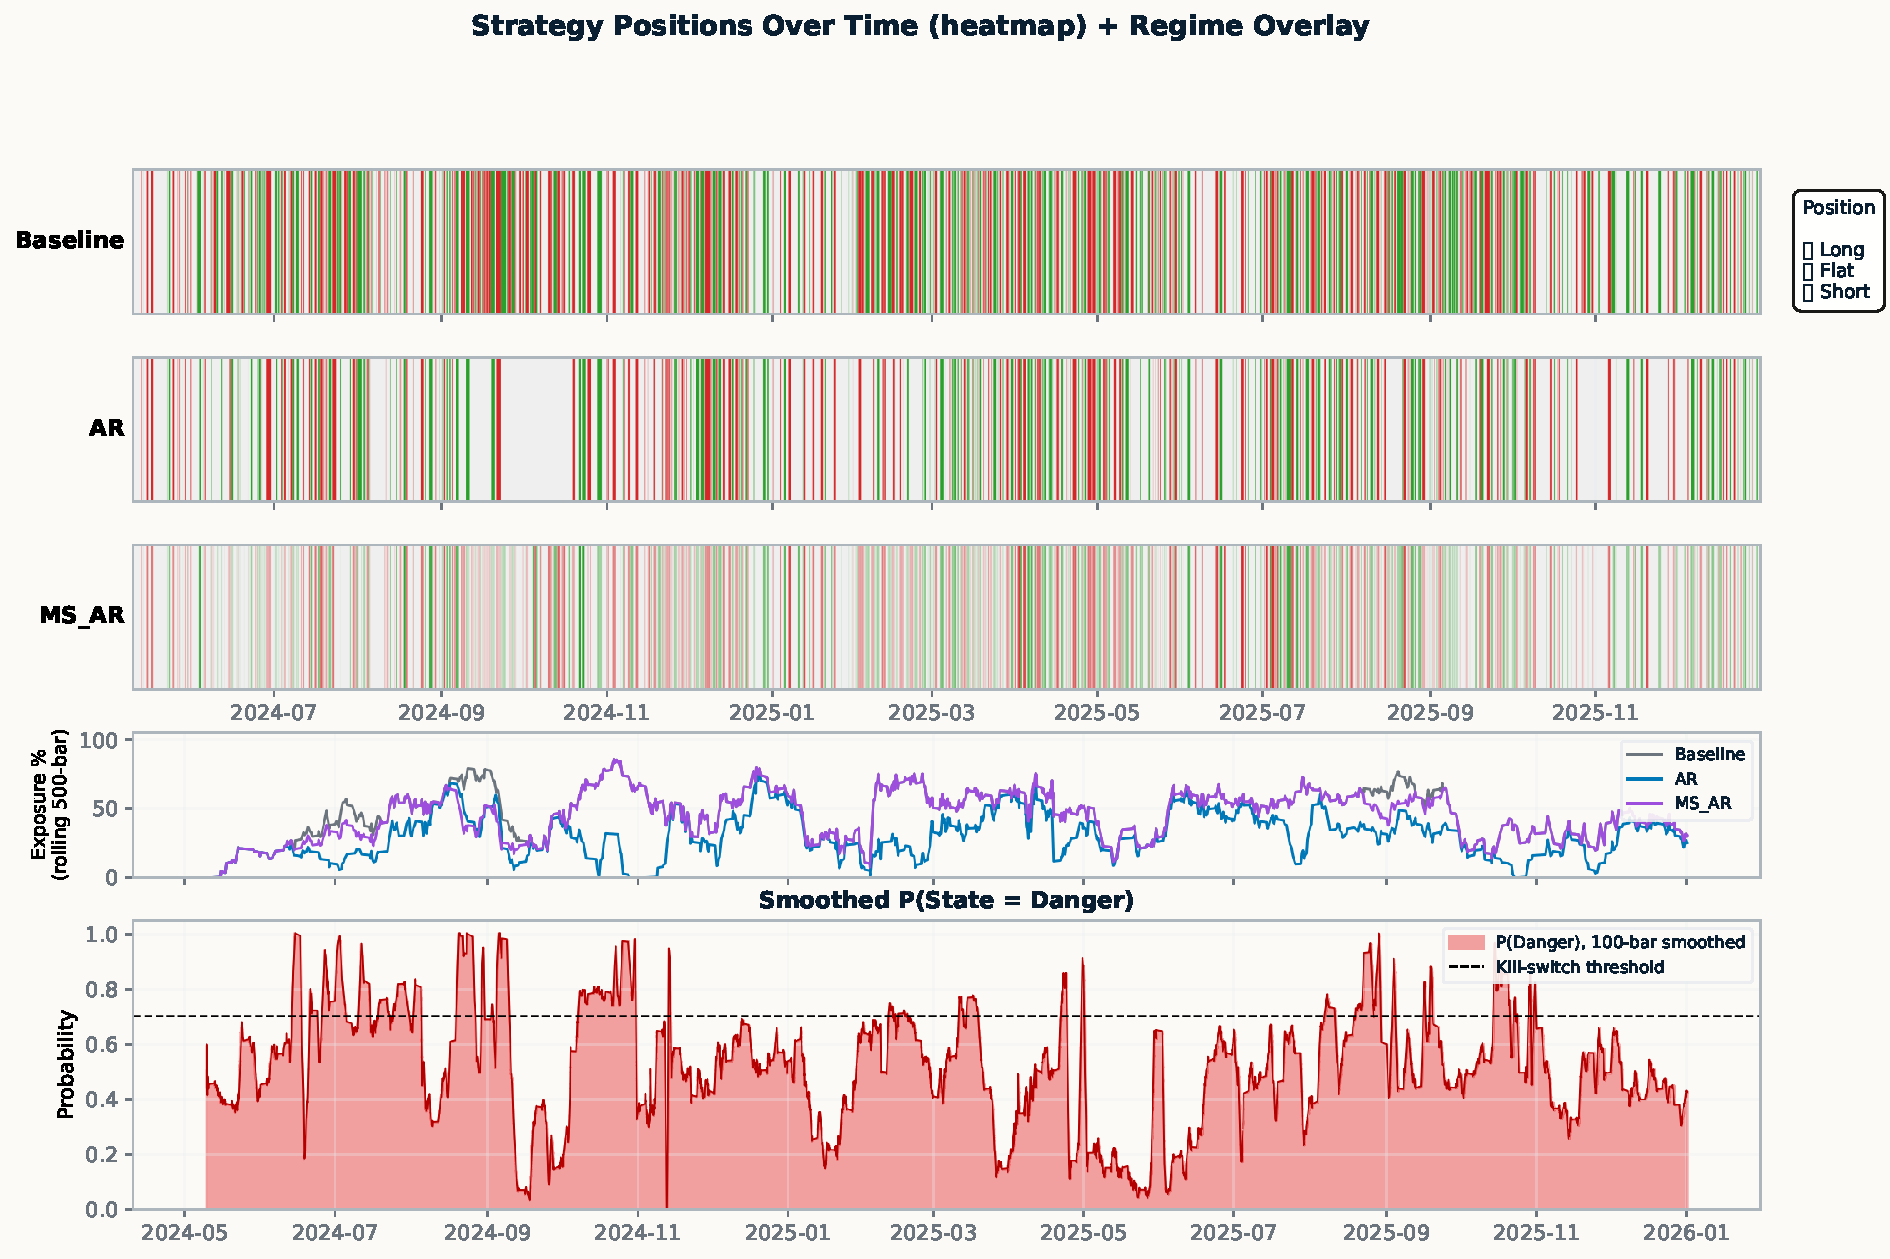
\includegraphics[width=\textwidth]{plots/GBPUSD_EURUSD_positions_and_regimes.pdf}
    \caption{Trading positions and regime overlays for GBPUSD/EURUSD. The figure shows exposure across the baseline, AR, and Markov-switching AR strategies, together with the smoothed dangerous-regime probability and the resulting long, flat, and short trading states.}
    \label{fig:GBPUSD_EURUSD_positions_and_regimes}
\end{figure}

%%%%%%%%%%%%%%%%%%%%%%%%%%%%%%%%%%%%%%%%%%%%%%%%%%%%%%%%%%%%%%
%%%%%%%%%%%%%%%%%%%%%%%%%%%%%%%%%%%%%%%%%%%%%%%%%%%%%%%%%%%%%%
%%%%%%%%%%%%%%%%%%%%%%%%%%%%%%%%%%%%%%%%%%%%%%%%%%%%%%%%%%%%%%



%%%%%%%%%%%%%%%%%%%%%%%%%%%%%%%%%%%%%%%%%%%%%%%%%%%%%%%%%%%%%%
%%%%%%%%%%%%%%%%%%%%%%%%%%%%%%%%%%%%%%%%%%%%%%%%%%%%%%%%%%%%%%
%%%%%%%%%%%%%%%%%%%%%%%%%%%%%%%%%%%%%%%%%%%%%%%%%%%%%%%%%%%%%%

\subsection{Cost impact}

\subsubsection{AUDUSD/NZDUSD}

\begin{figure}[H]
    \centering
    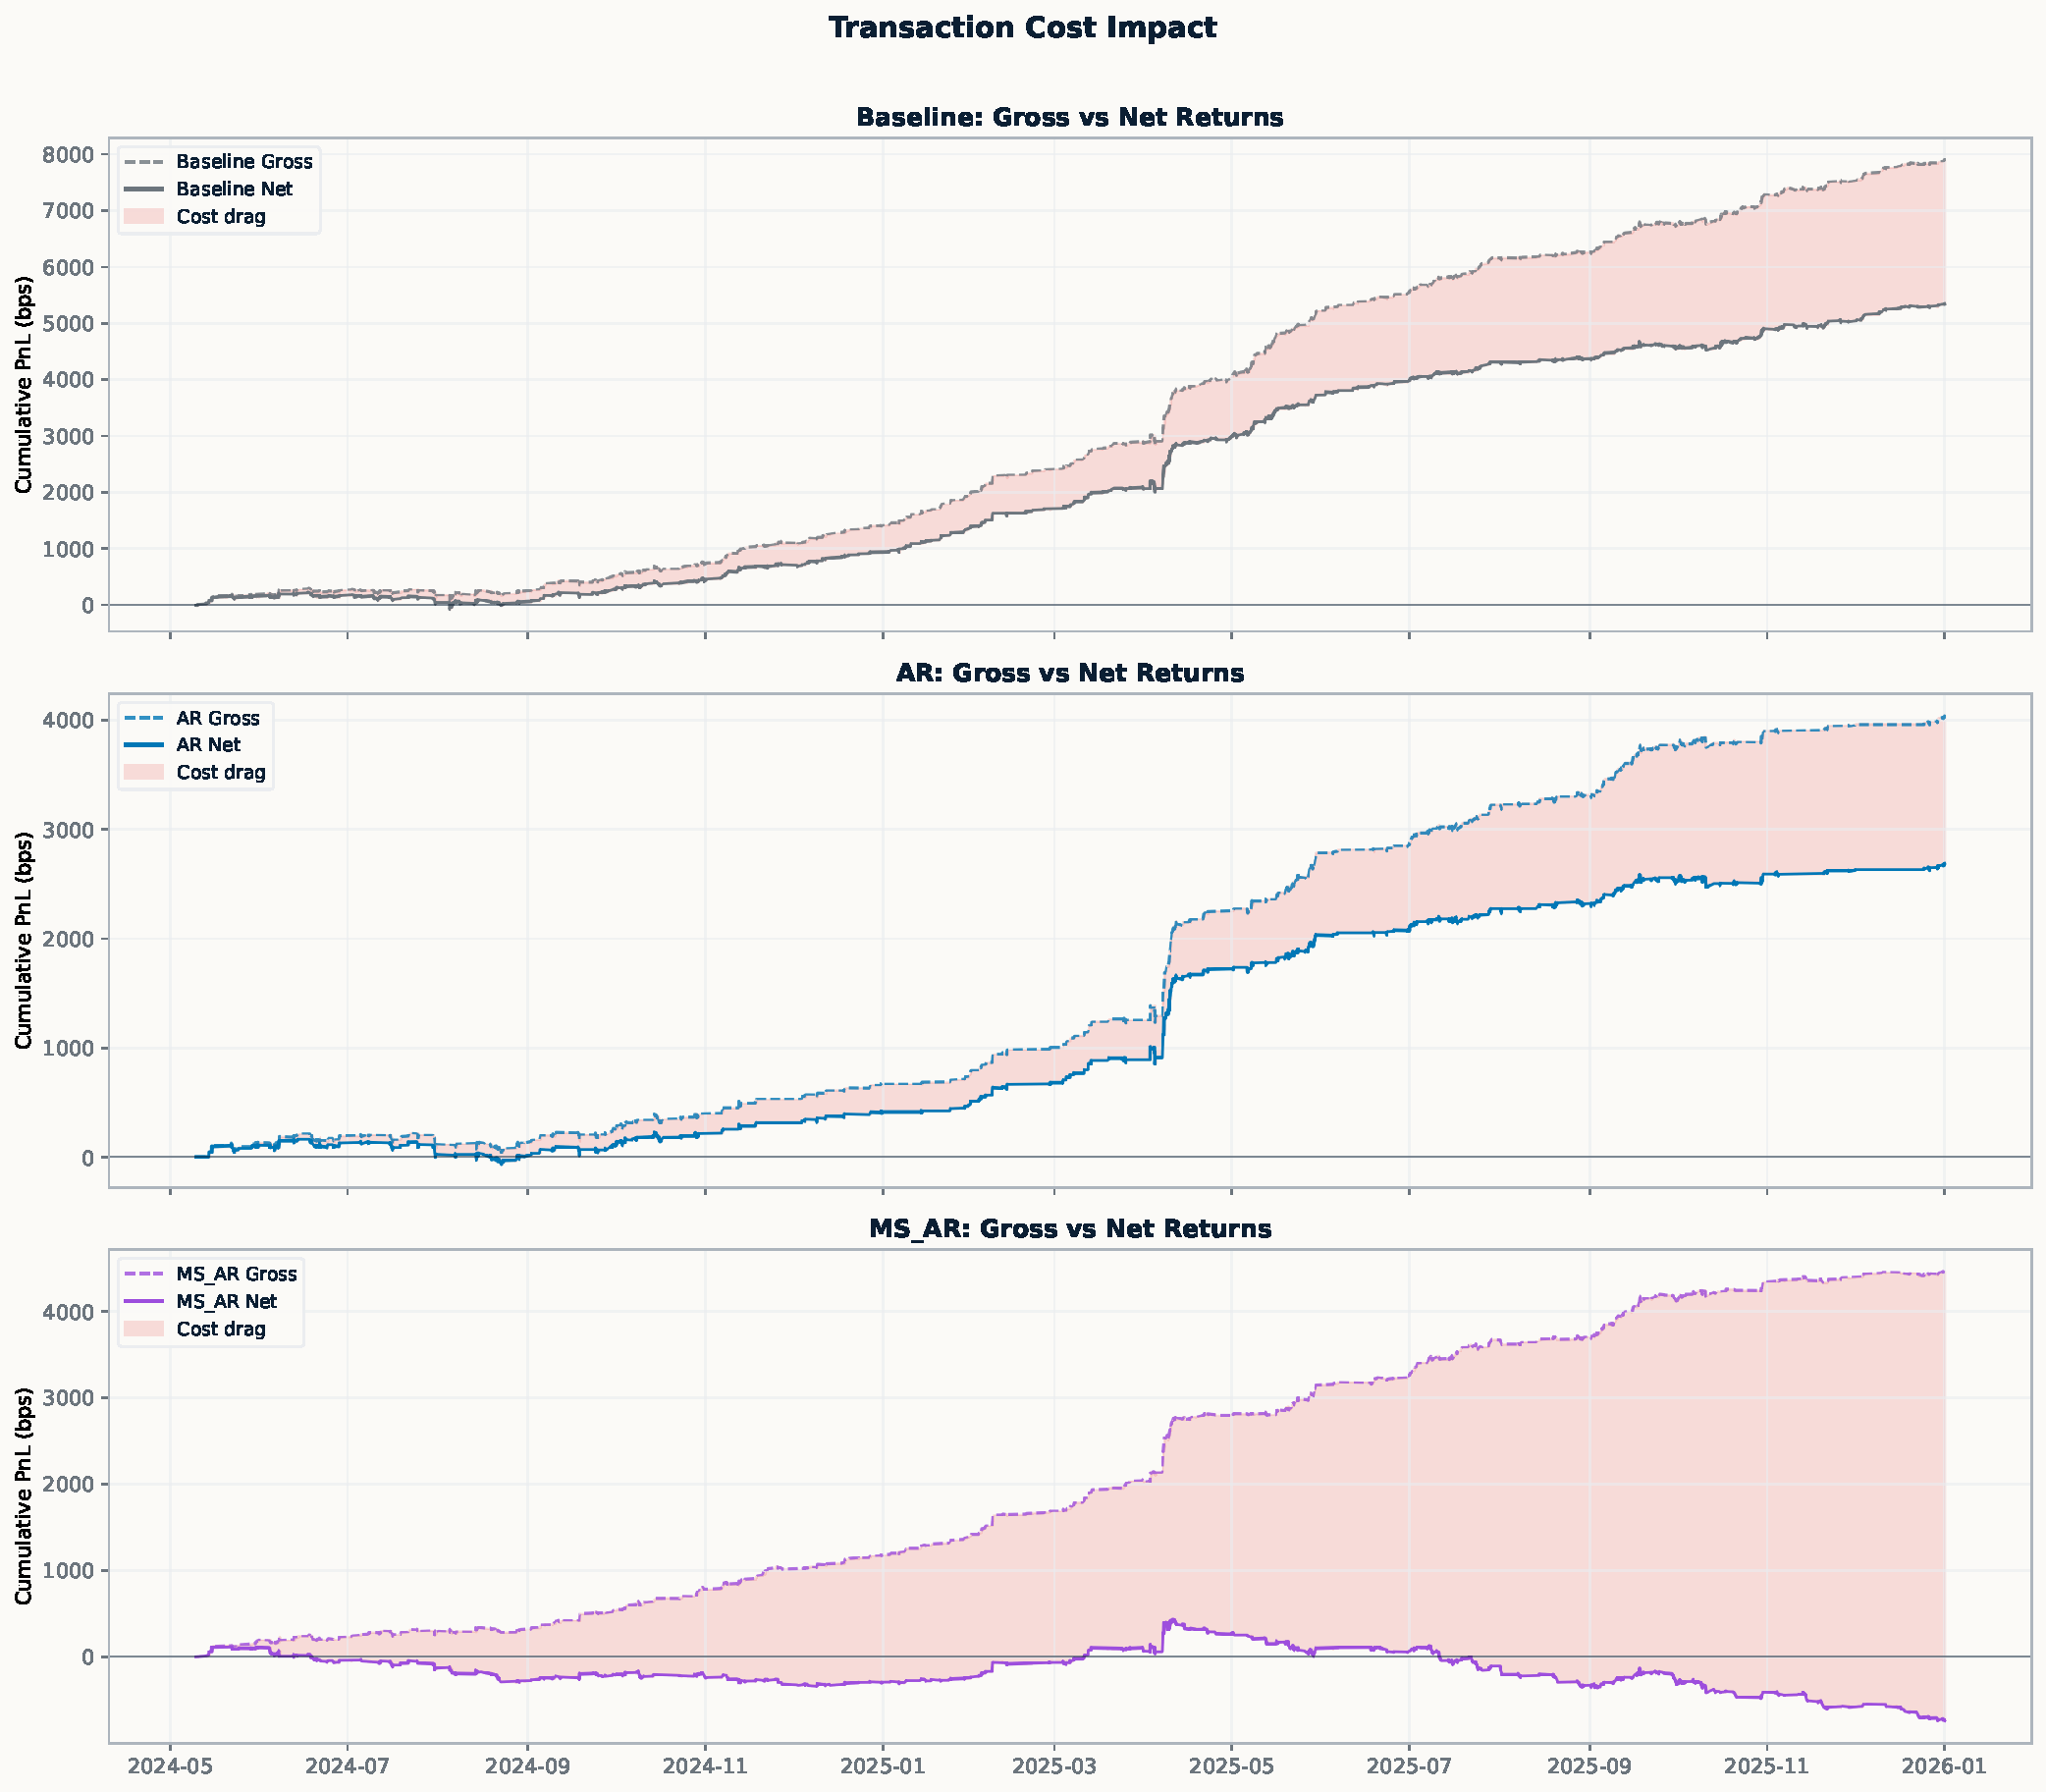
\includegraphics[width=\textwidth]{plots/AUDUSD_NZDUSD_cost_impact.pdf}
    \caption{Cost impact for AUDUSD/NZDUSD. The figure shows how transaction costs affect strategy performance for the baseline, AR, and Markov-switching AR strategies, highlighting the sensitivity of cumulative returns to implementation frictions.}
    \label{fig:AUDUSD_NZDUSD_cost_impact}
\end{figure}

\subsubsection{EURNOK/EURSEK}

\begin{figure}[H]
    \centering
    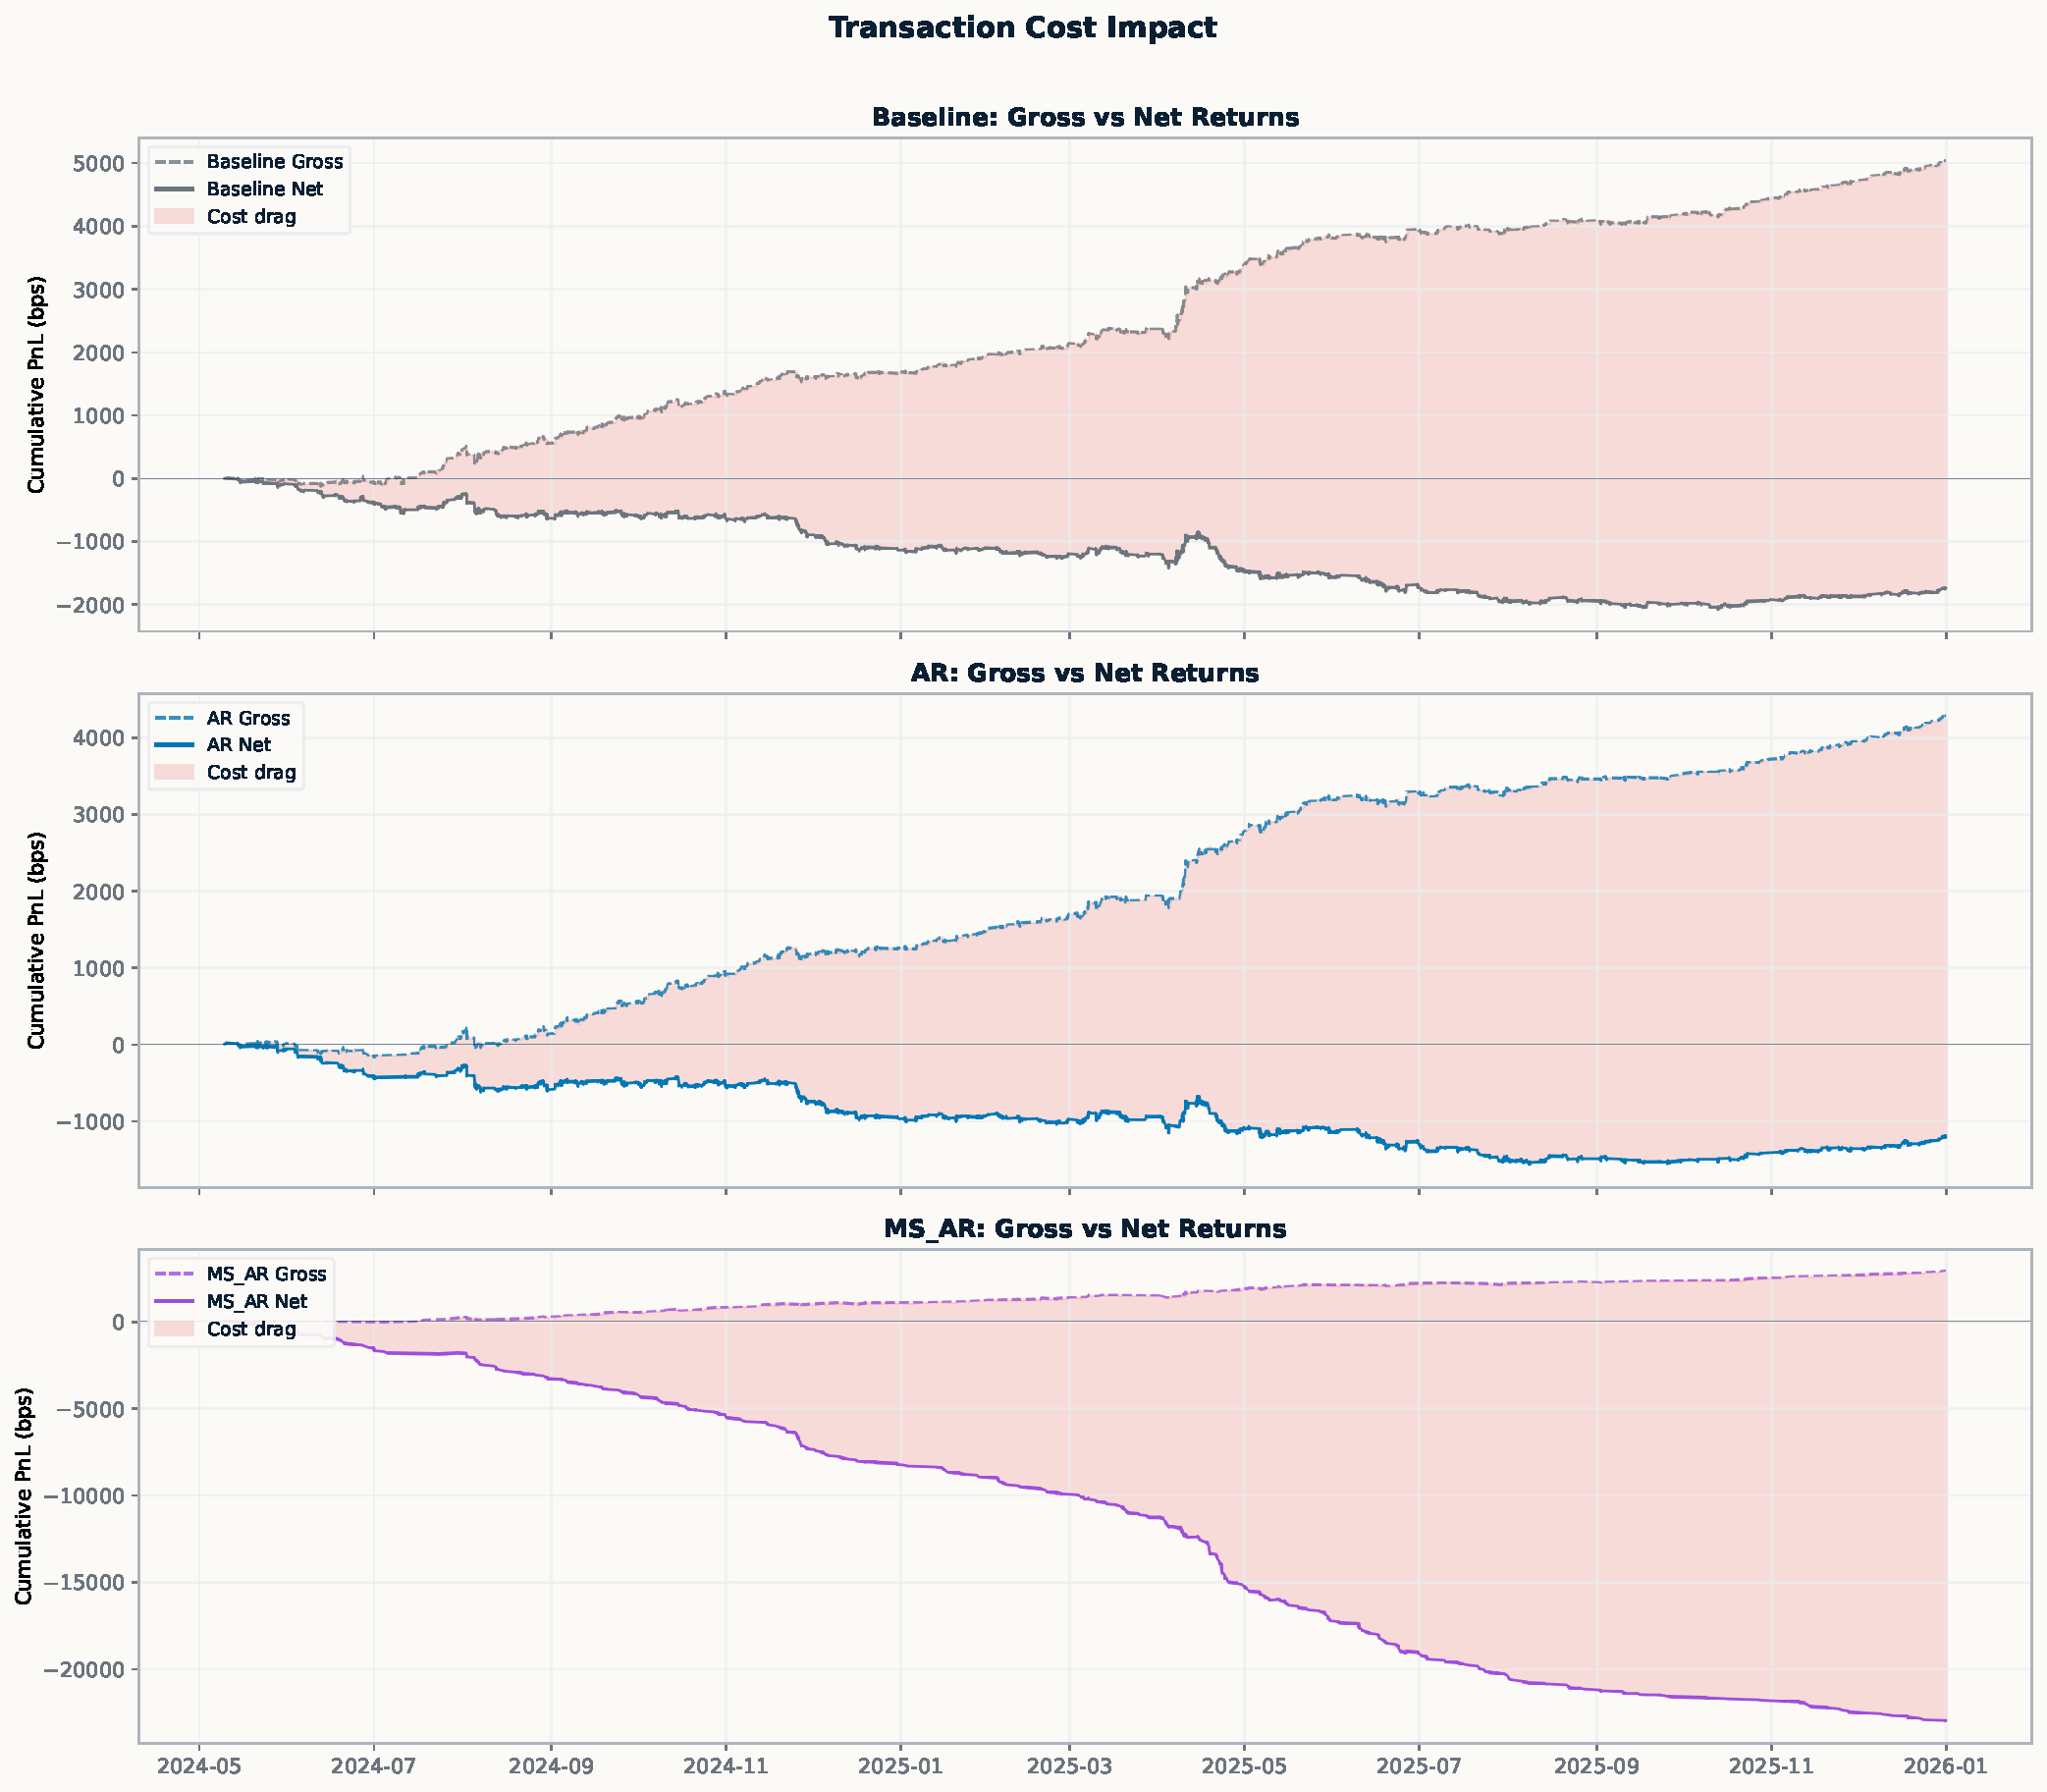
\includegraphics[width=\textwidth]{plots/EURNOK_EURSEK_cost_impact.pdf}
    \caption{Cost impact for EURNOK/EURSEK. The figure shows how transaction costs affect strategy performance for the baseline, AR, and Markov-switching AR strategies, highlighting the sensitivity of cumulative returns to implementation frictions.}
    \label{fig:EURNOK_EURSEK_cost_impact}
\end{figure}

\subsubsection{GBPUSD/EURUSD}

\begin{figure}[H]
    \centering
    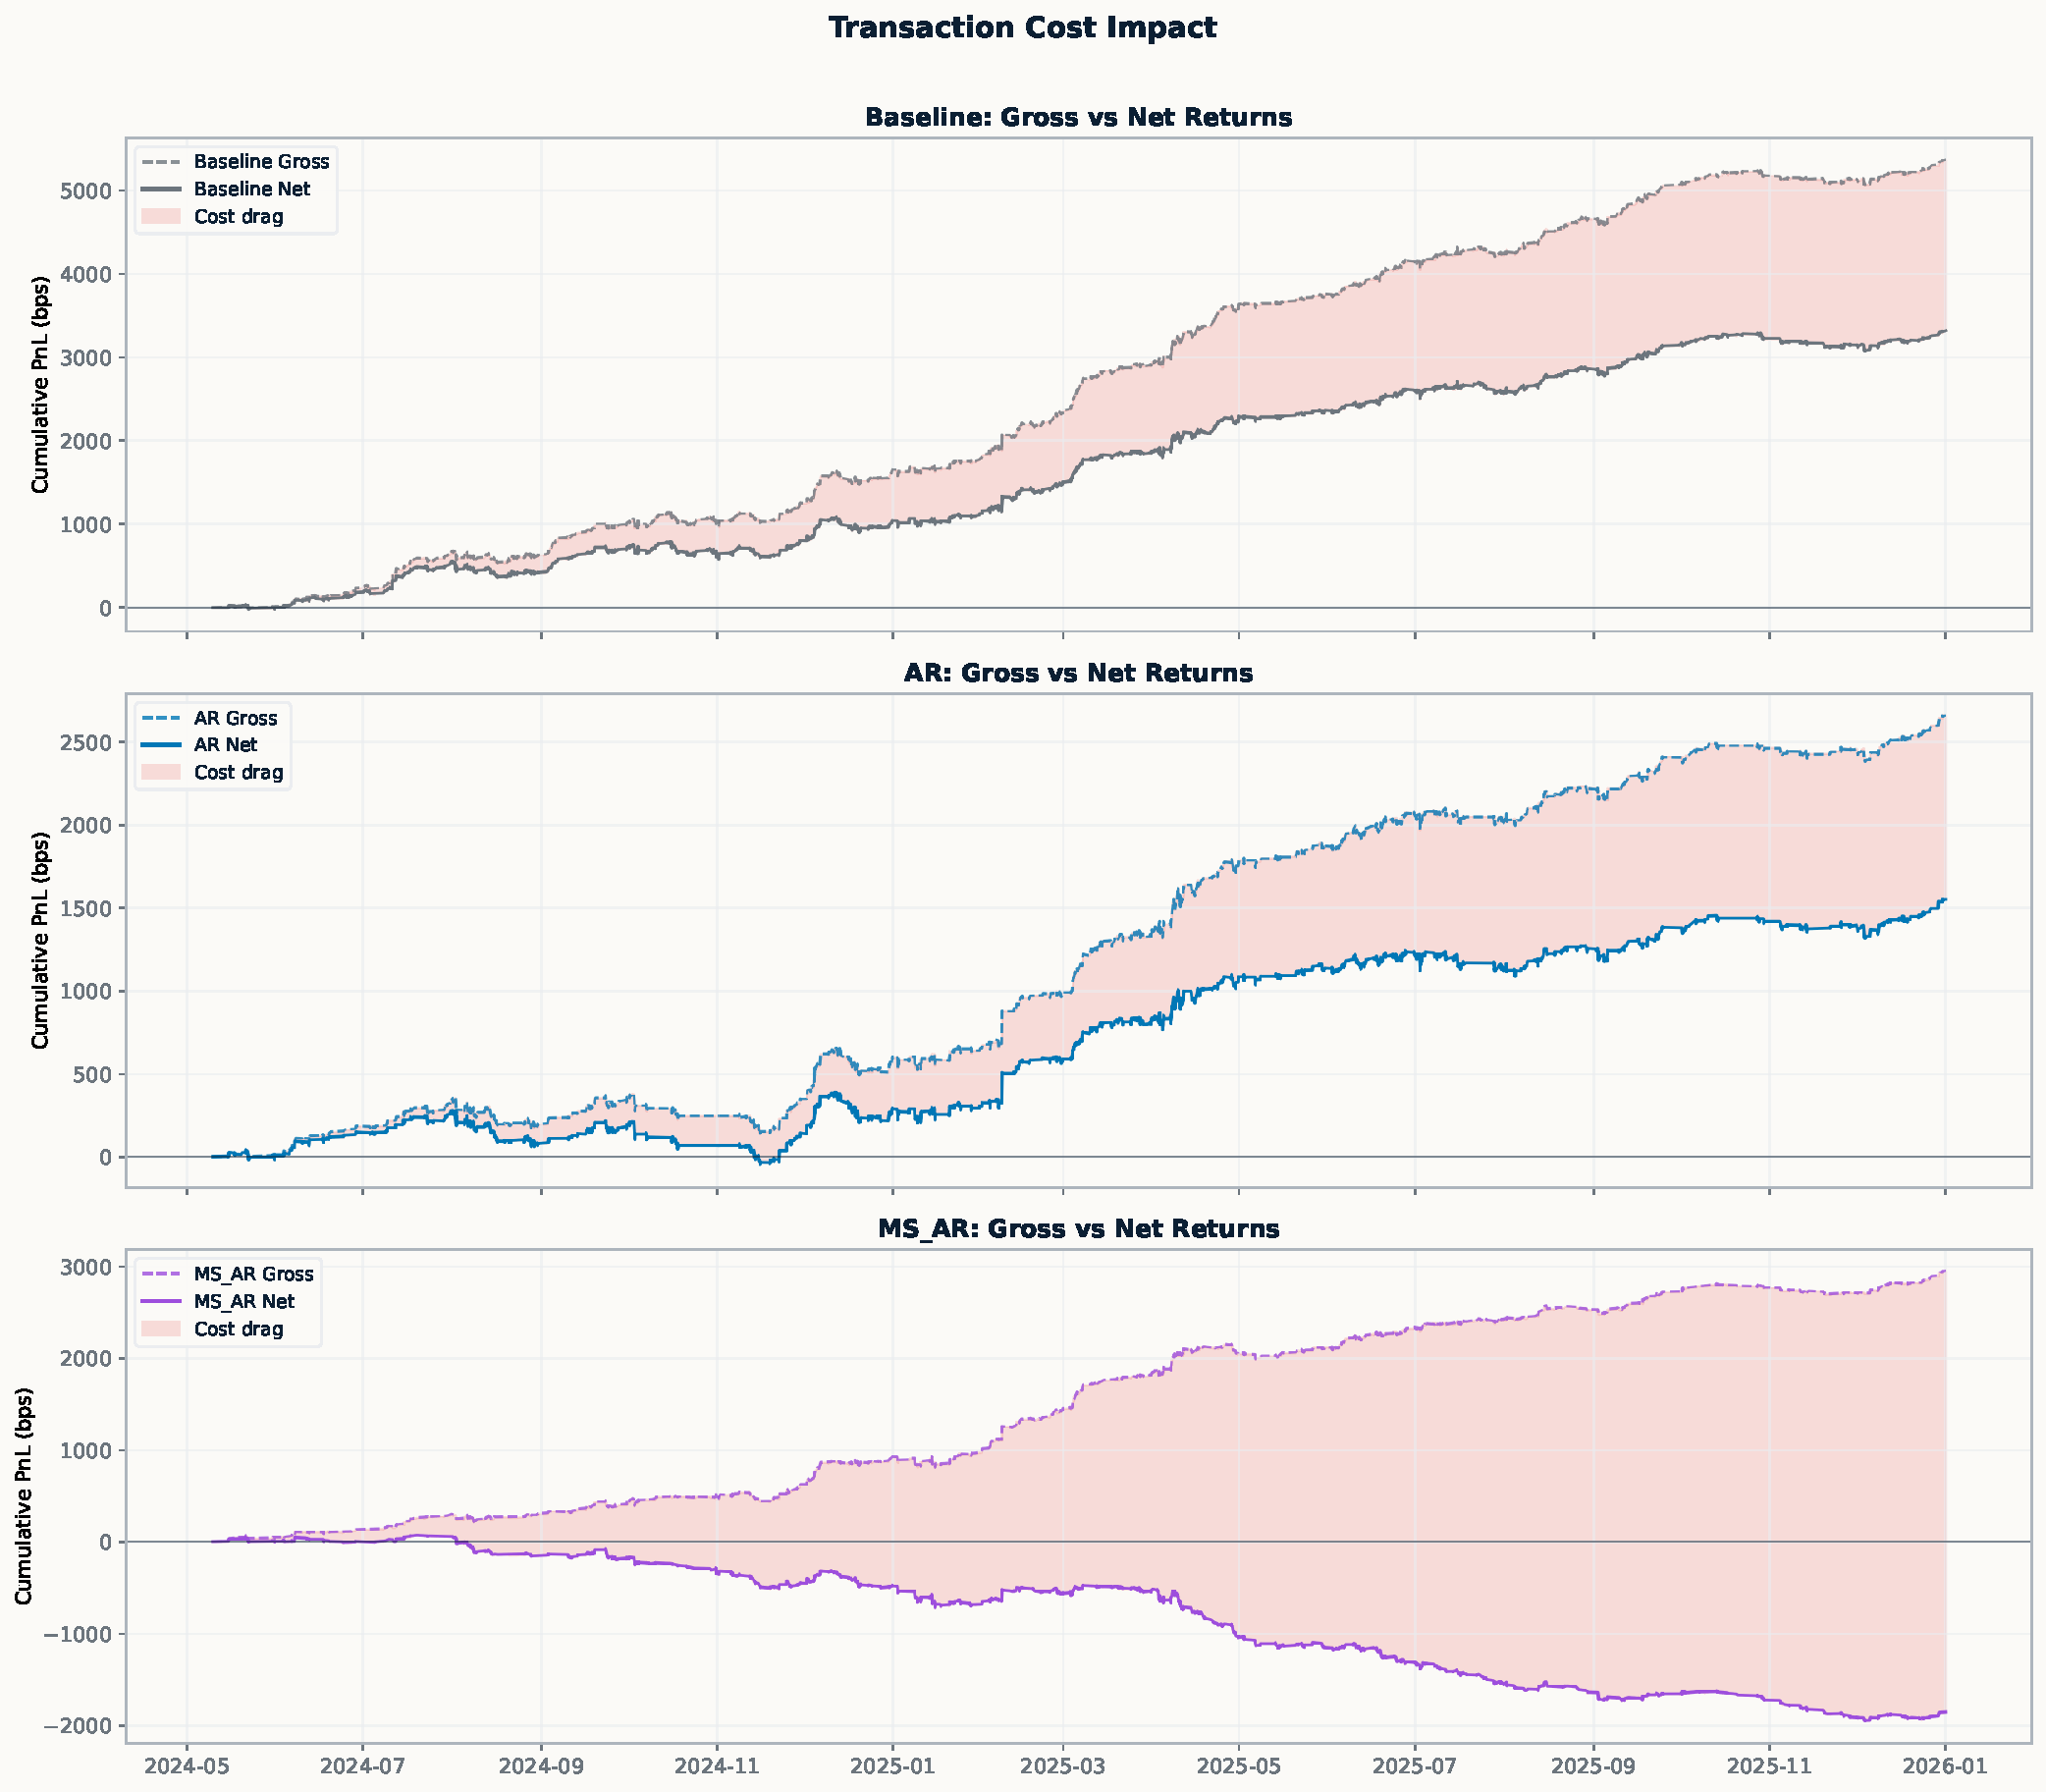
\includegraphics[width=\textwidth]{plots/GBPUSD_EURUSD_cost_impact.pdf}
    \caption{Cost impact for GBPUSD/EURUSD. The figure shows how transaction costs affect strategy performance for the baseline, AR, and Markov-switching AR strategies, highlighting the sensitivity of cumulative returns to implementation frictions.}
    \label{fig:GBPUSD_EURUSD_cost_impact}
\end{figure}

%%%%%%%%%%%%%%%%%%%%%%%%%%%%%%%%%%%%%%%%%%%%%%%%%%%%%%%%%%%%%%
%%%%%%%%%%%%%%%%%%%%%%%%%%%%%%%%%%%%%%%%%%%%%%%%%%%%%%%%%%%%%%
%%%%%%%%%%%%%%%%%%%%%%%%%%%%%%%%%%%%%%%%%%%%%%%%%%%%%%%%%%%%%%

\subsection{Daily positions and regimes}

\subsubsection{AUDUSD/NZDUSD}

\begin{figure}[H]
    \centering
    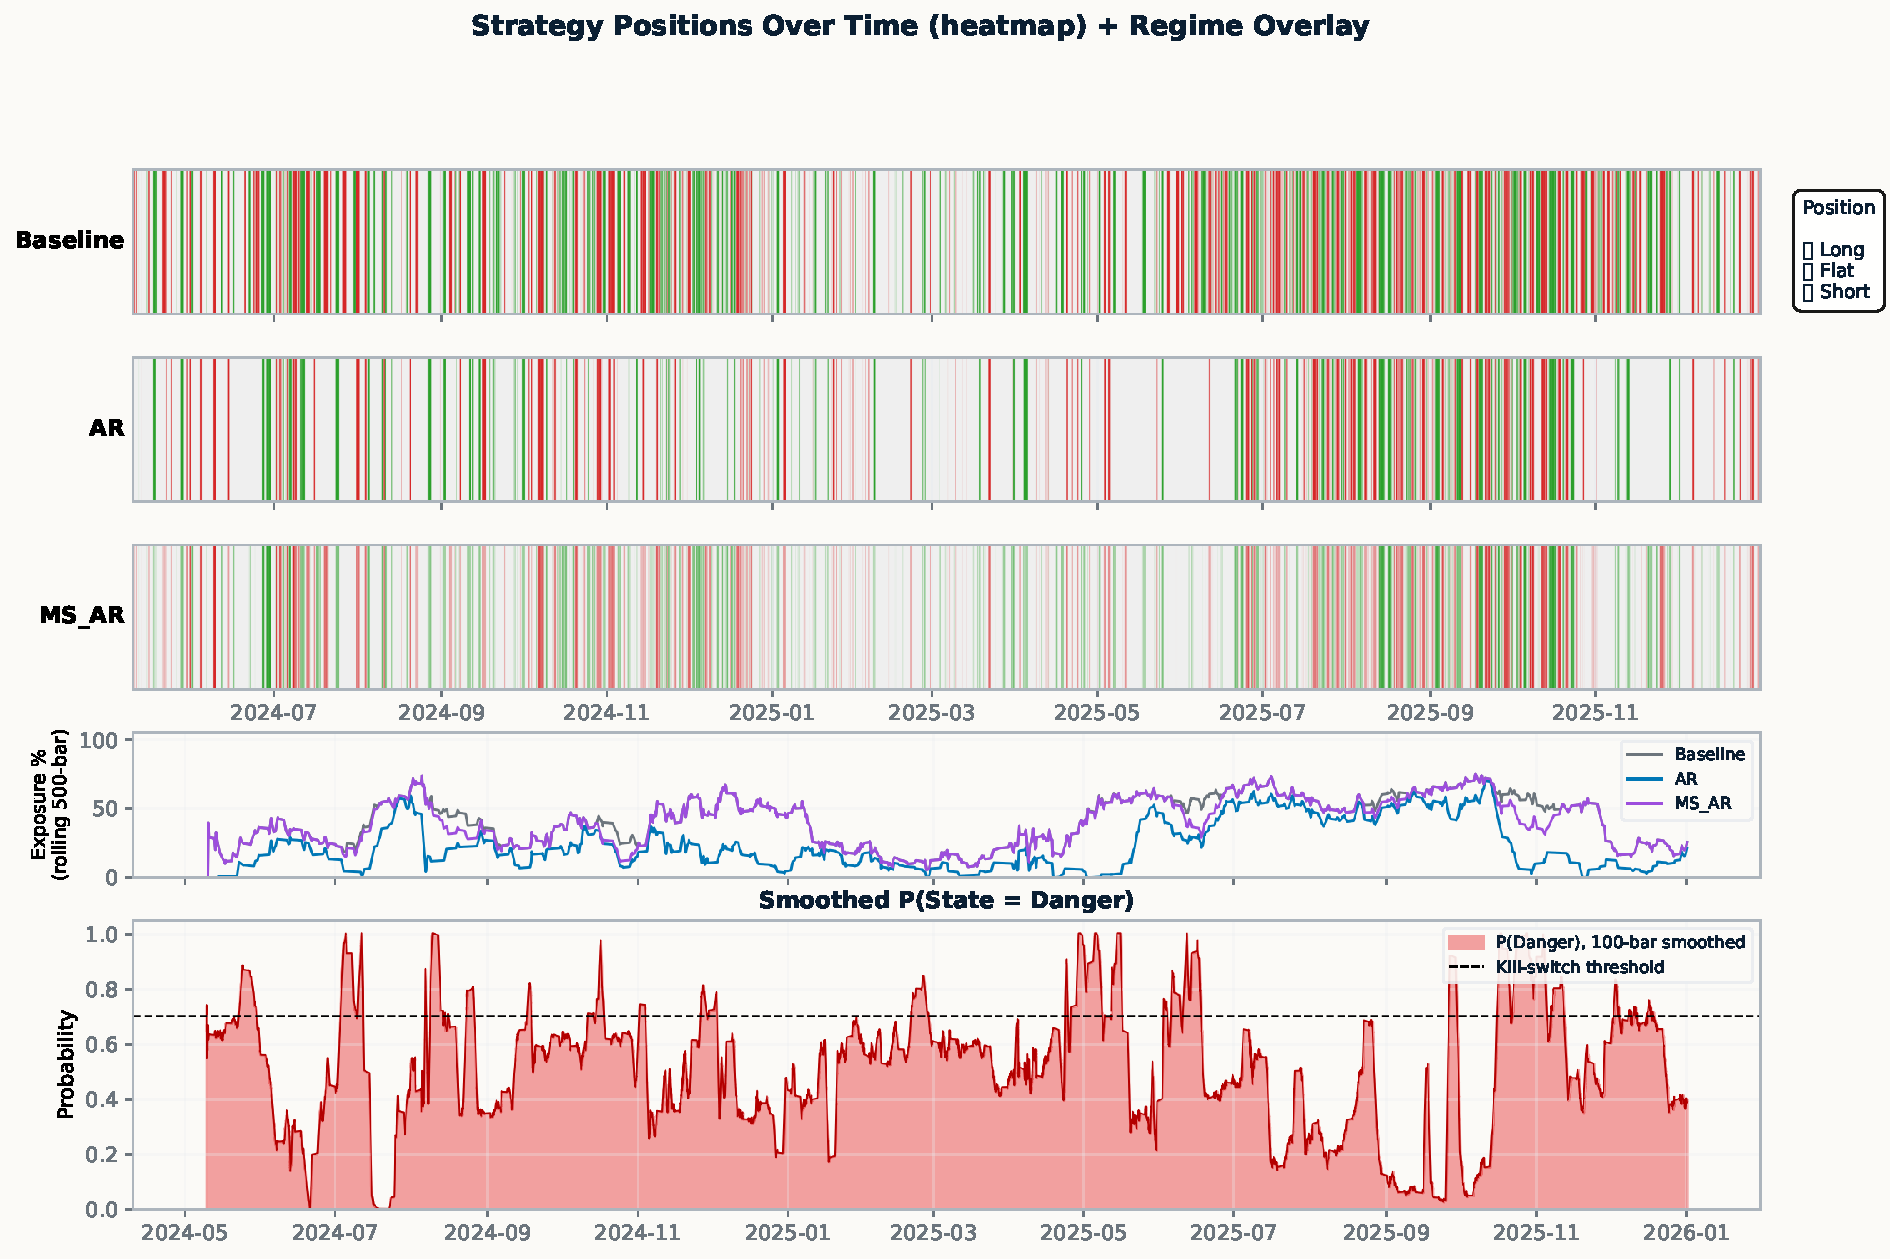
\includegraphics[width=\textwidth]{plots/AUDUSD_NZDUSD_daily_positions_and_regimes.pdf}
    \caption{Daily positions and regime overlays for AUDUSD/NZDUSD. The figure shows daily trading exposure across the baseline, AR, and Markov-switching AR strategies, together with the smoothed dangerous-regime probability and the resulting long, flat, and short trading states.}
    \label{fig:AUDUSD_NZDUSD_daily_positions_and_regimes}
\end{figure}

\subsubsection{EURNOK/EURSEK}

\begin{figure}[H]
    \centering
    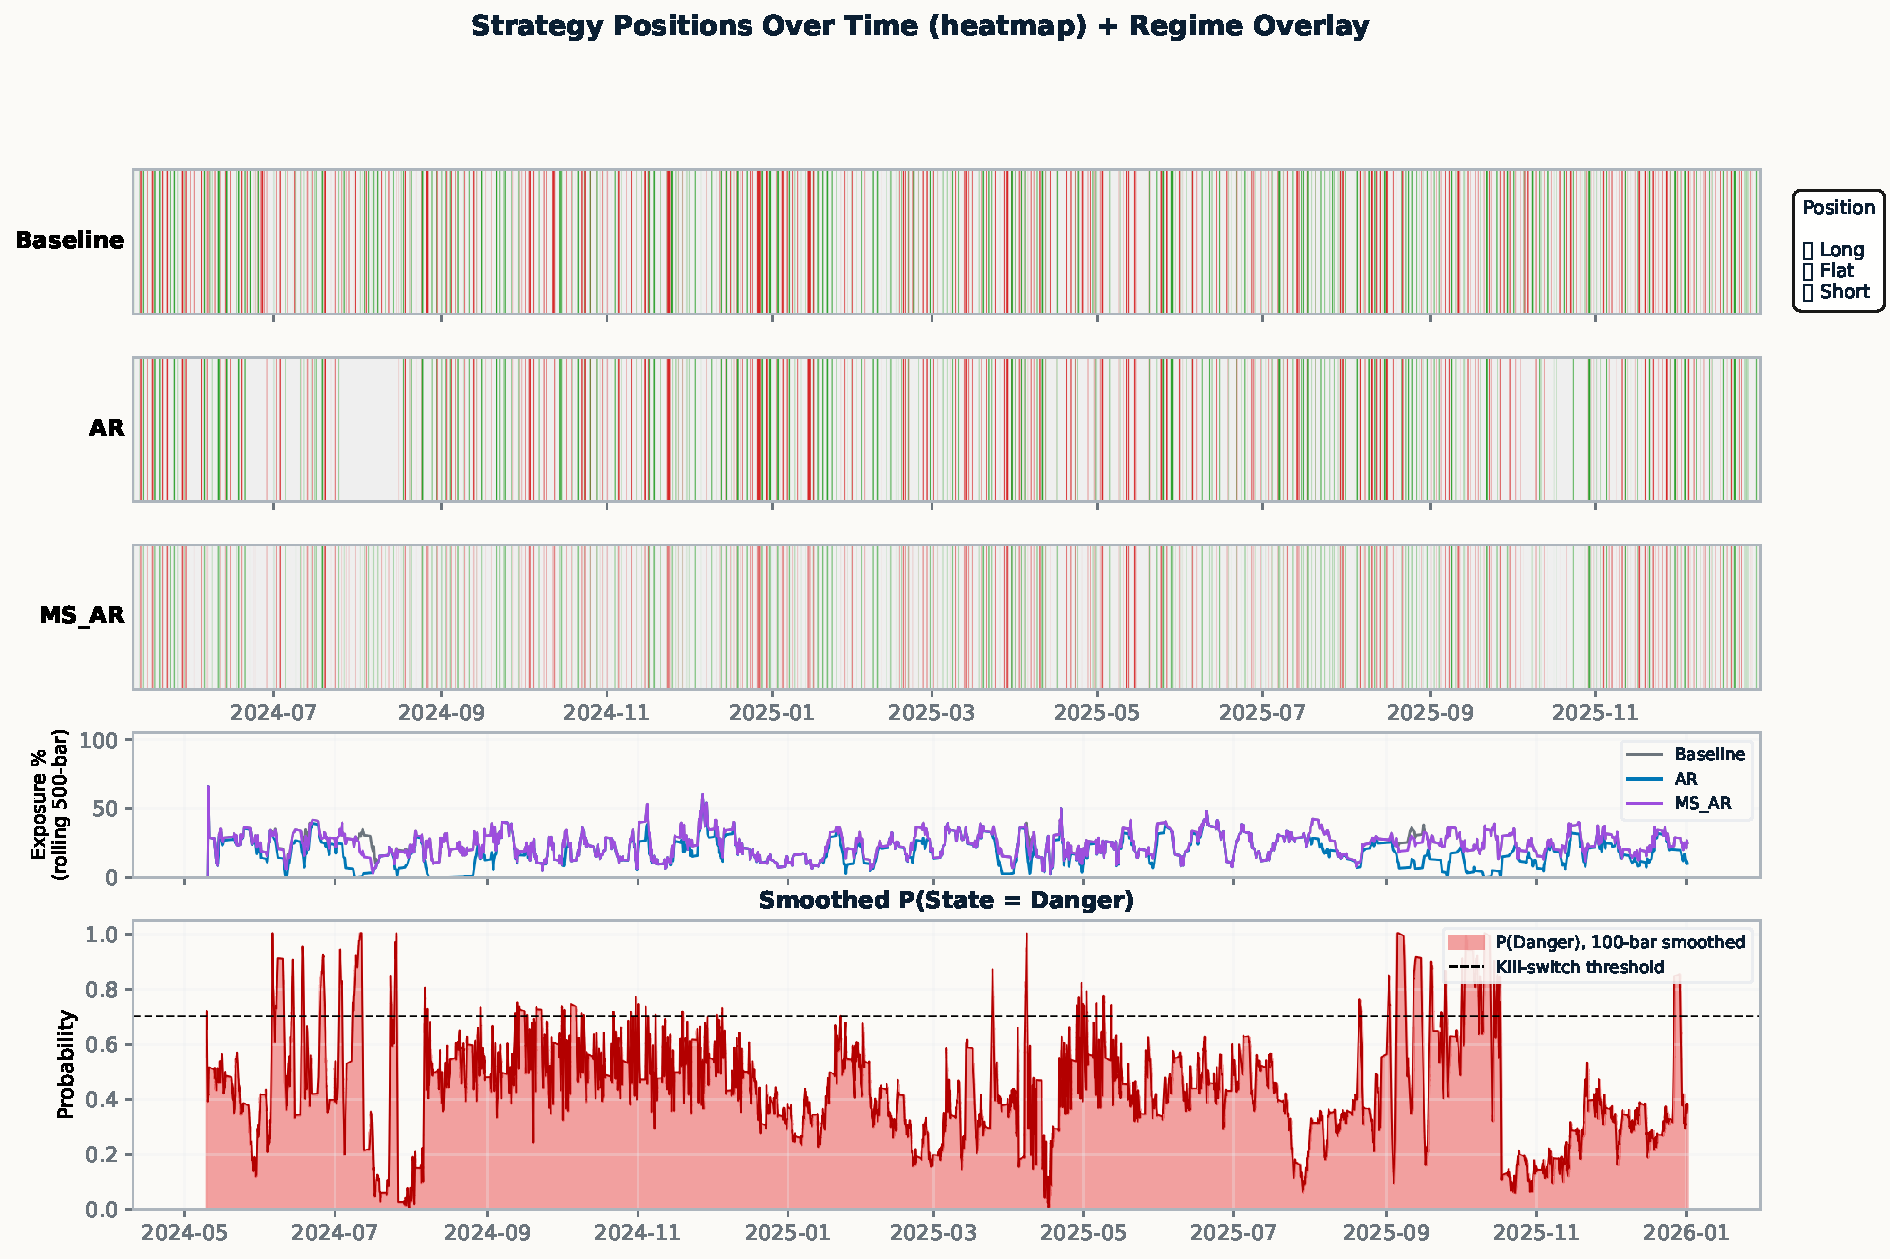
\includegraphics[width=\textwidth]{plots/EURNOK_EURSEK_daily_positions_and_regimes.pdf}
    \caption{Daily positions and regime overlays for EURNOK/EURSEK. The figure shows daily trading exposure across the baseline, AR, and Markov-switching AR strategies, together with the smoothed dangerous-regime probability and the resulting long, flat, and short trading states.}
    \label{fig:EURNOK_EURSEK_daily_positions_and_regimes}
\end{figure}

\subsubsection{GBPUSD/EURUSD}

\begin{figure}[H]
    \centering
    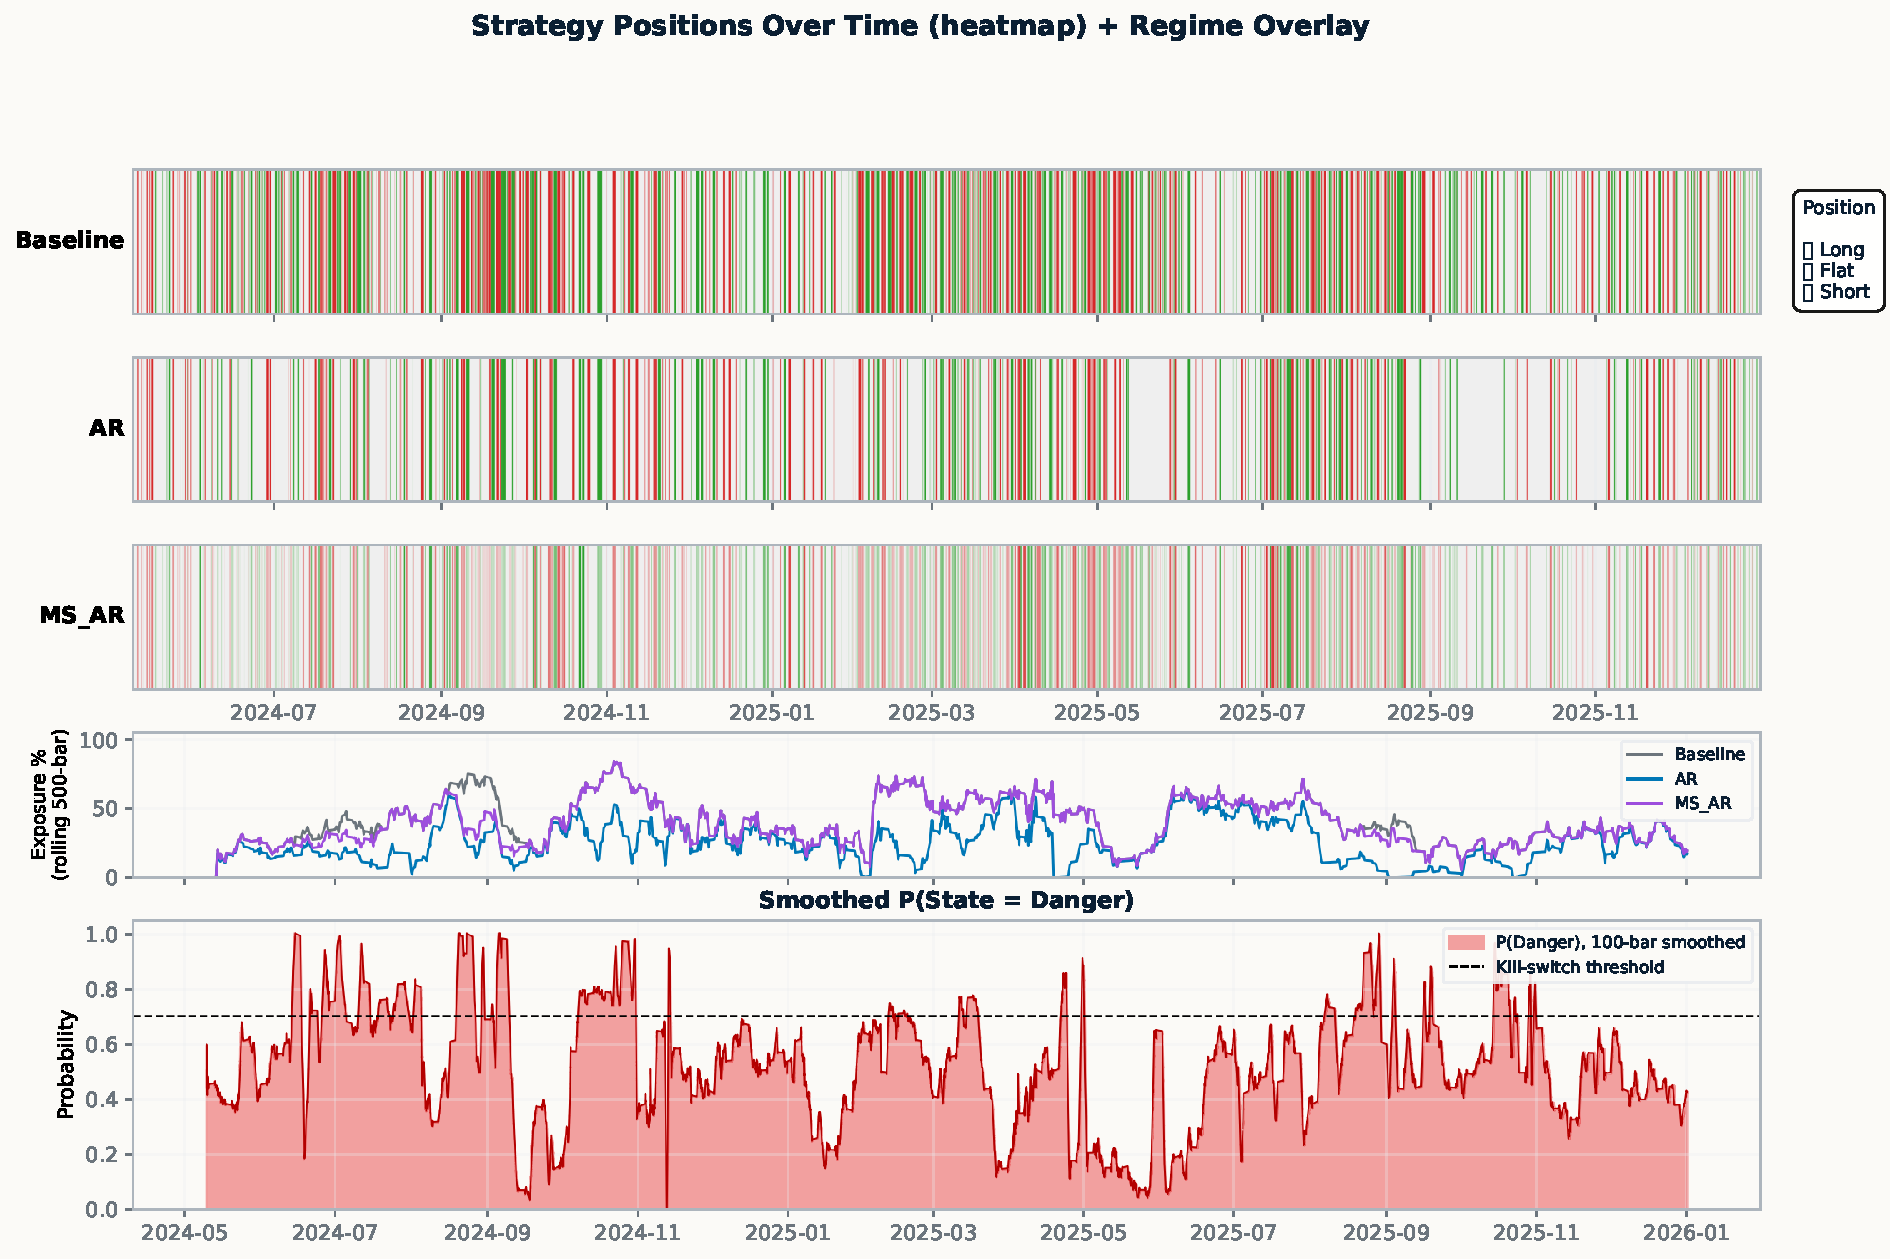
\includegraphics[width=\textwidth]{plots/GBPUSD_EURUSD_daily_positions_and_regimes.pdf}
    \caption{Daily positions and regime overlays for GBPUSD/EURUSD. The figure shows daily trading exposure across the baseline, AR, and Markov-switching AR strategies, together with the smoothed dangerous-regime probability and the resulting long, flat, and short trading states.}
    \label{fig:GBPUSD_EURUSD_daily_positions_and_regimes}
\end{figure}

%%%%%%%%%%%%%%%%%%%%%%%%%%%%%%%%%%%%%%%%%%%%%%%%%%%%%%%%%%%%%%
%%%%%%%%%%%%%%%%%%%%%%%%%%%%%%%%%%%%%%%%%%%%%%%%%%%%%%%%%%%%%%
%%%%%%%%%%%%%%%%%%%%%%%%%%%%%%%%%%%%%%%%%%%%%%%%%%%%%%%%%%%%%%


\subsection{Daily backtest performance}

\subsubsection{AUDUSD/NZDUSD}

\begin{figure}[H]
    \centering
    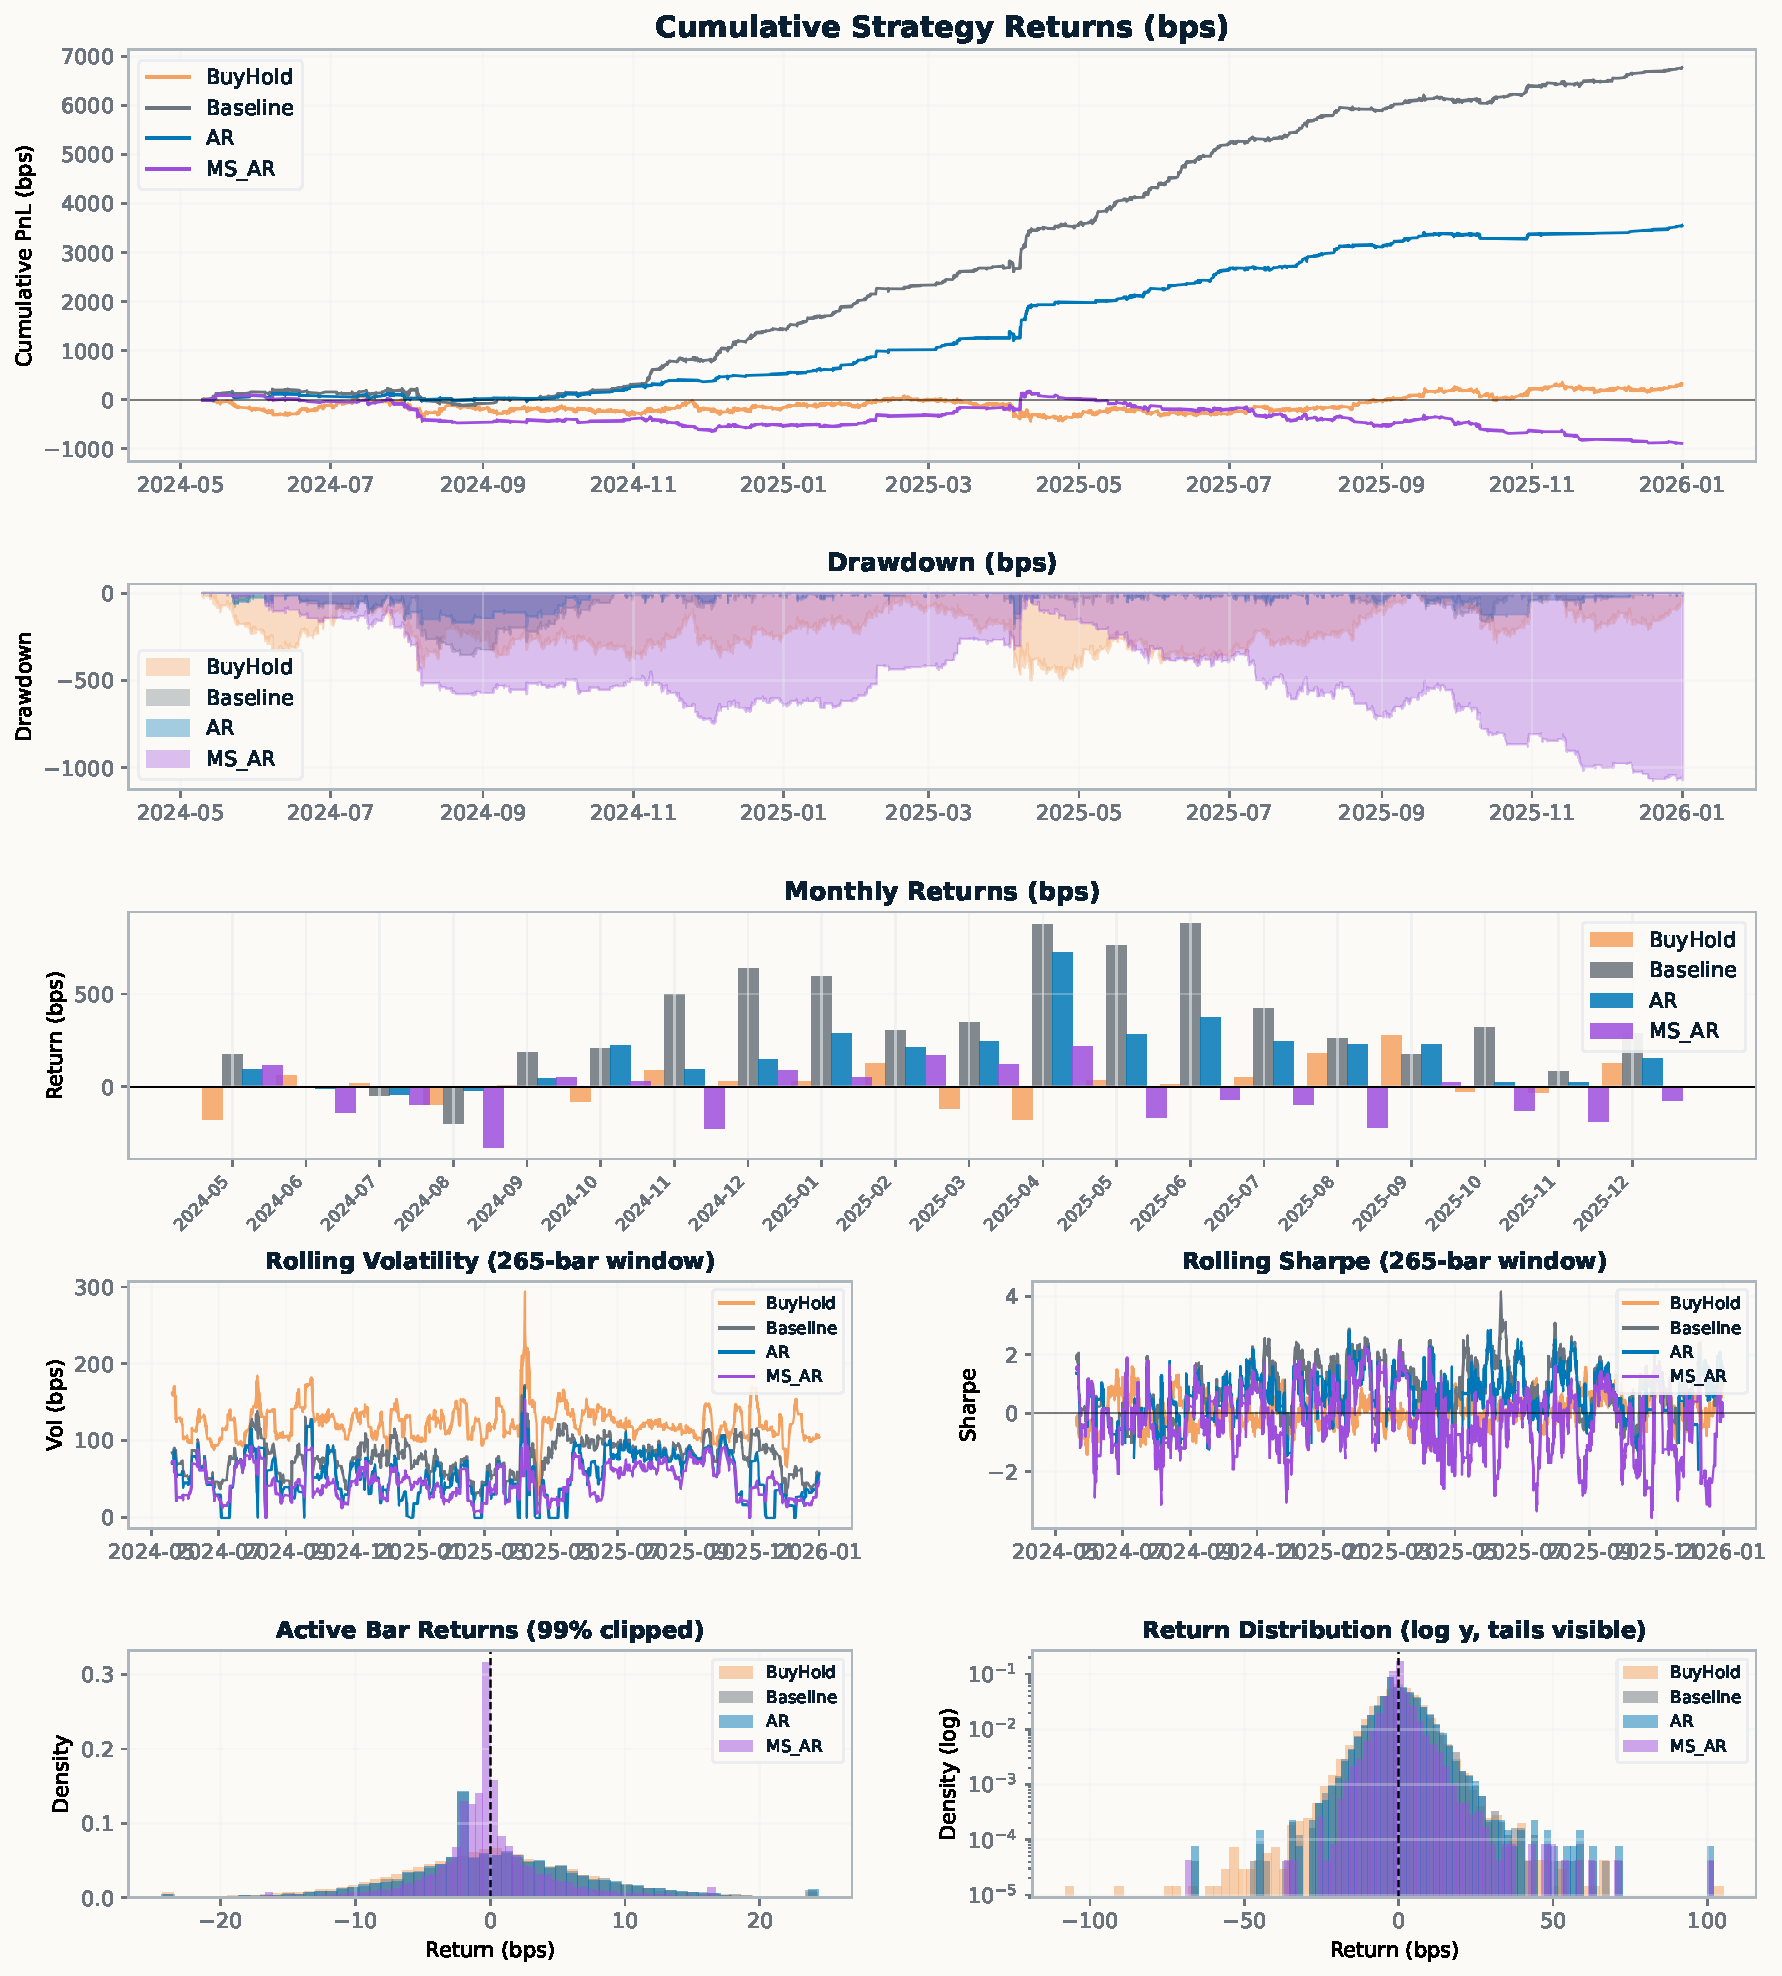
\includegraphics[width=\textwidth]{plots/AUDUSD_NZDUSD_daily_performance.pdf}
    \caption{Daily backtest performance for AUDUSD/NZDUSD across the baseline, AR, and Markov-switching AR strategies. The figure compares cumulative strategy returns, drawdowns, monthly returns, rolling volatility, rolling Sharpe ratios, active-day return distributions, and tail behaviour on a log-density scale.}
    \label{fig:AUDUSD_NZDUSD_daily_performance}
\end{figure}

\subsubsection{EURNOK/EURSEK}

\begin{figure}[H]
    \centering
    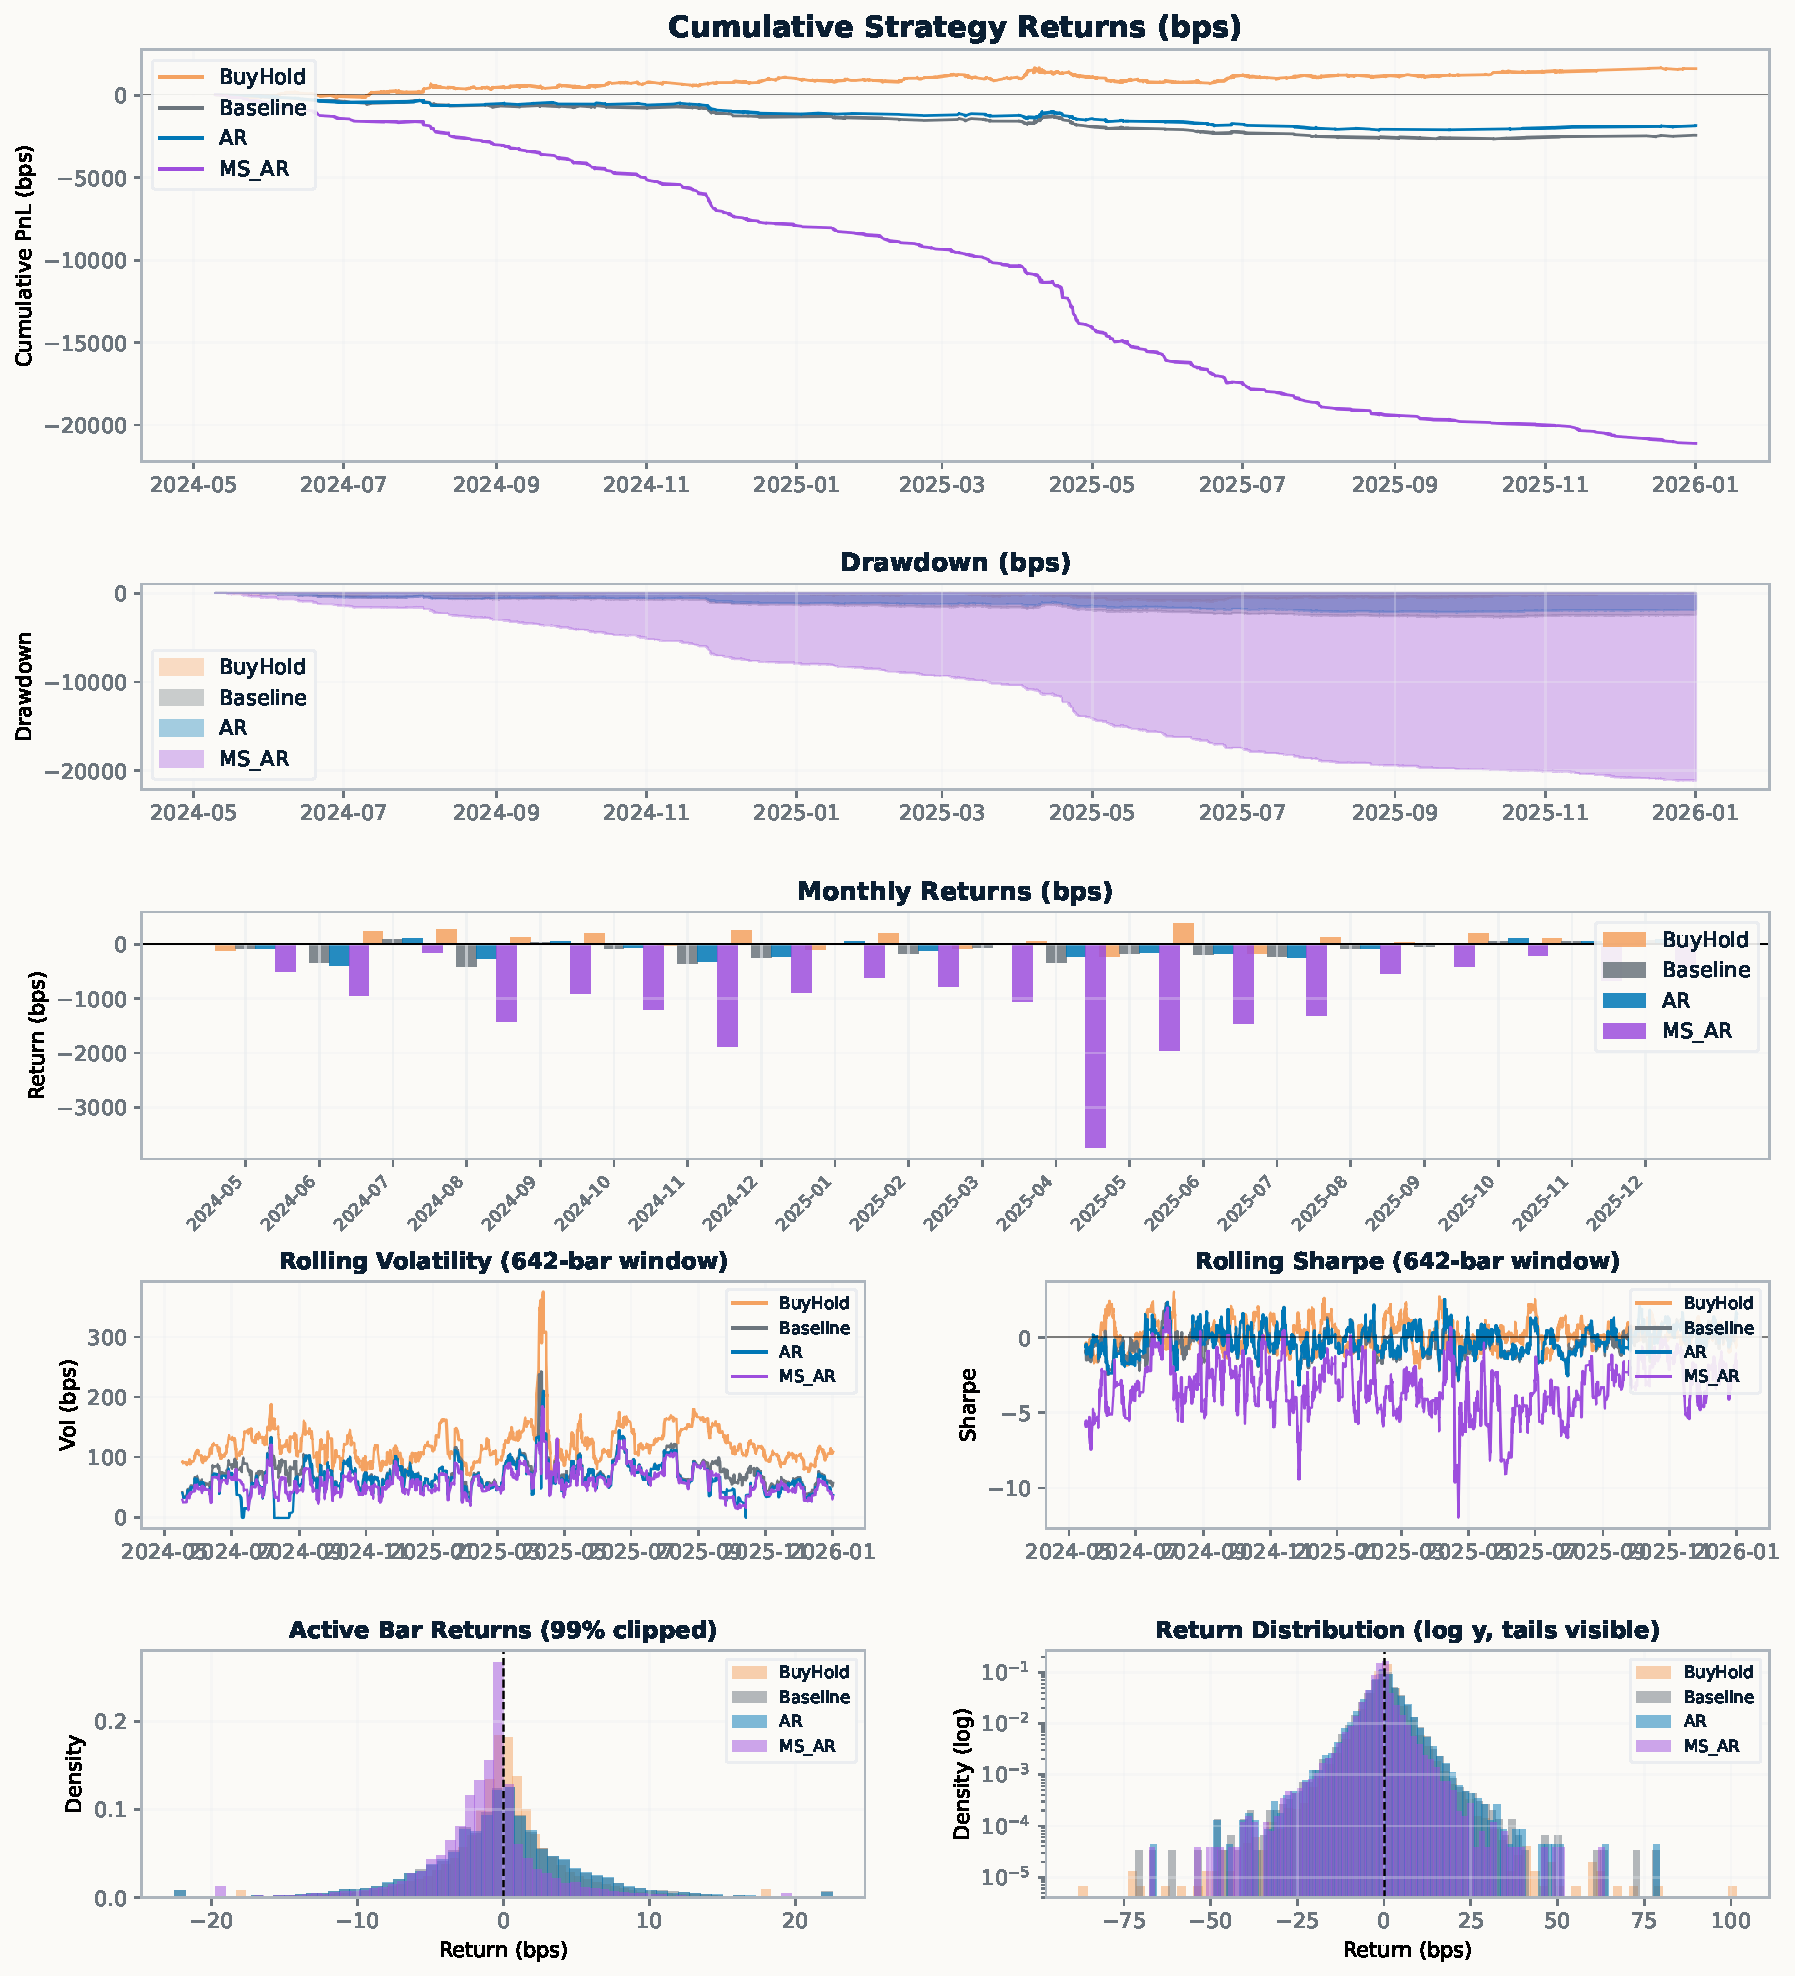
\includegraphics[width=\textwidth]{plots/EURNOK_EURSEK_daily_performance.pdf}
    \caption{Daily backtest performance for EURNOK/EURSEK across the baseline, AR, and Markov-switching AR strategies. The figure compares cumulative returns, drawdowns, monthly return contributions, rolling volatility, rolling Sharpe ratios, active-day return densities, and tail behaviour.}
    \label{fig:EURNOK_EURSEK_daily_performance}
\end{figure}

\subsubsection{GBPUSD/EURUSD}

\begin{figure}[H]
    \centering
    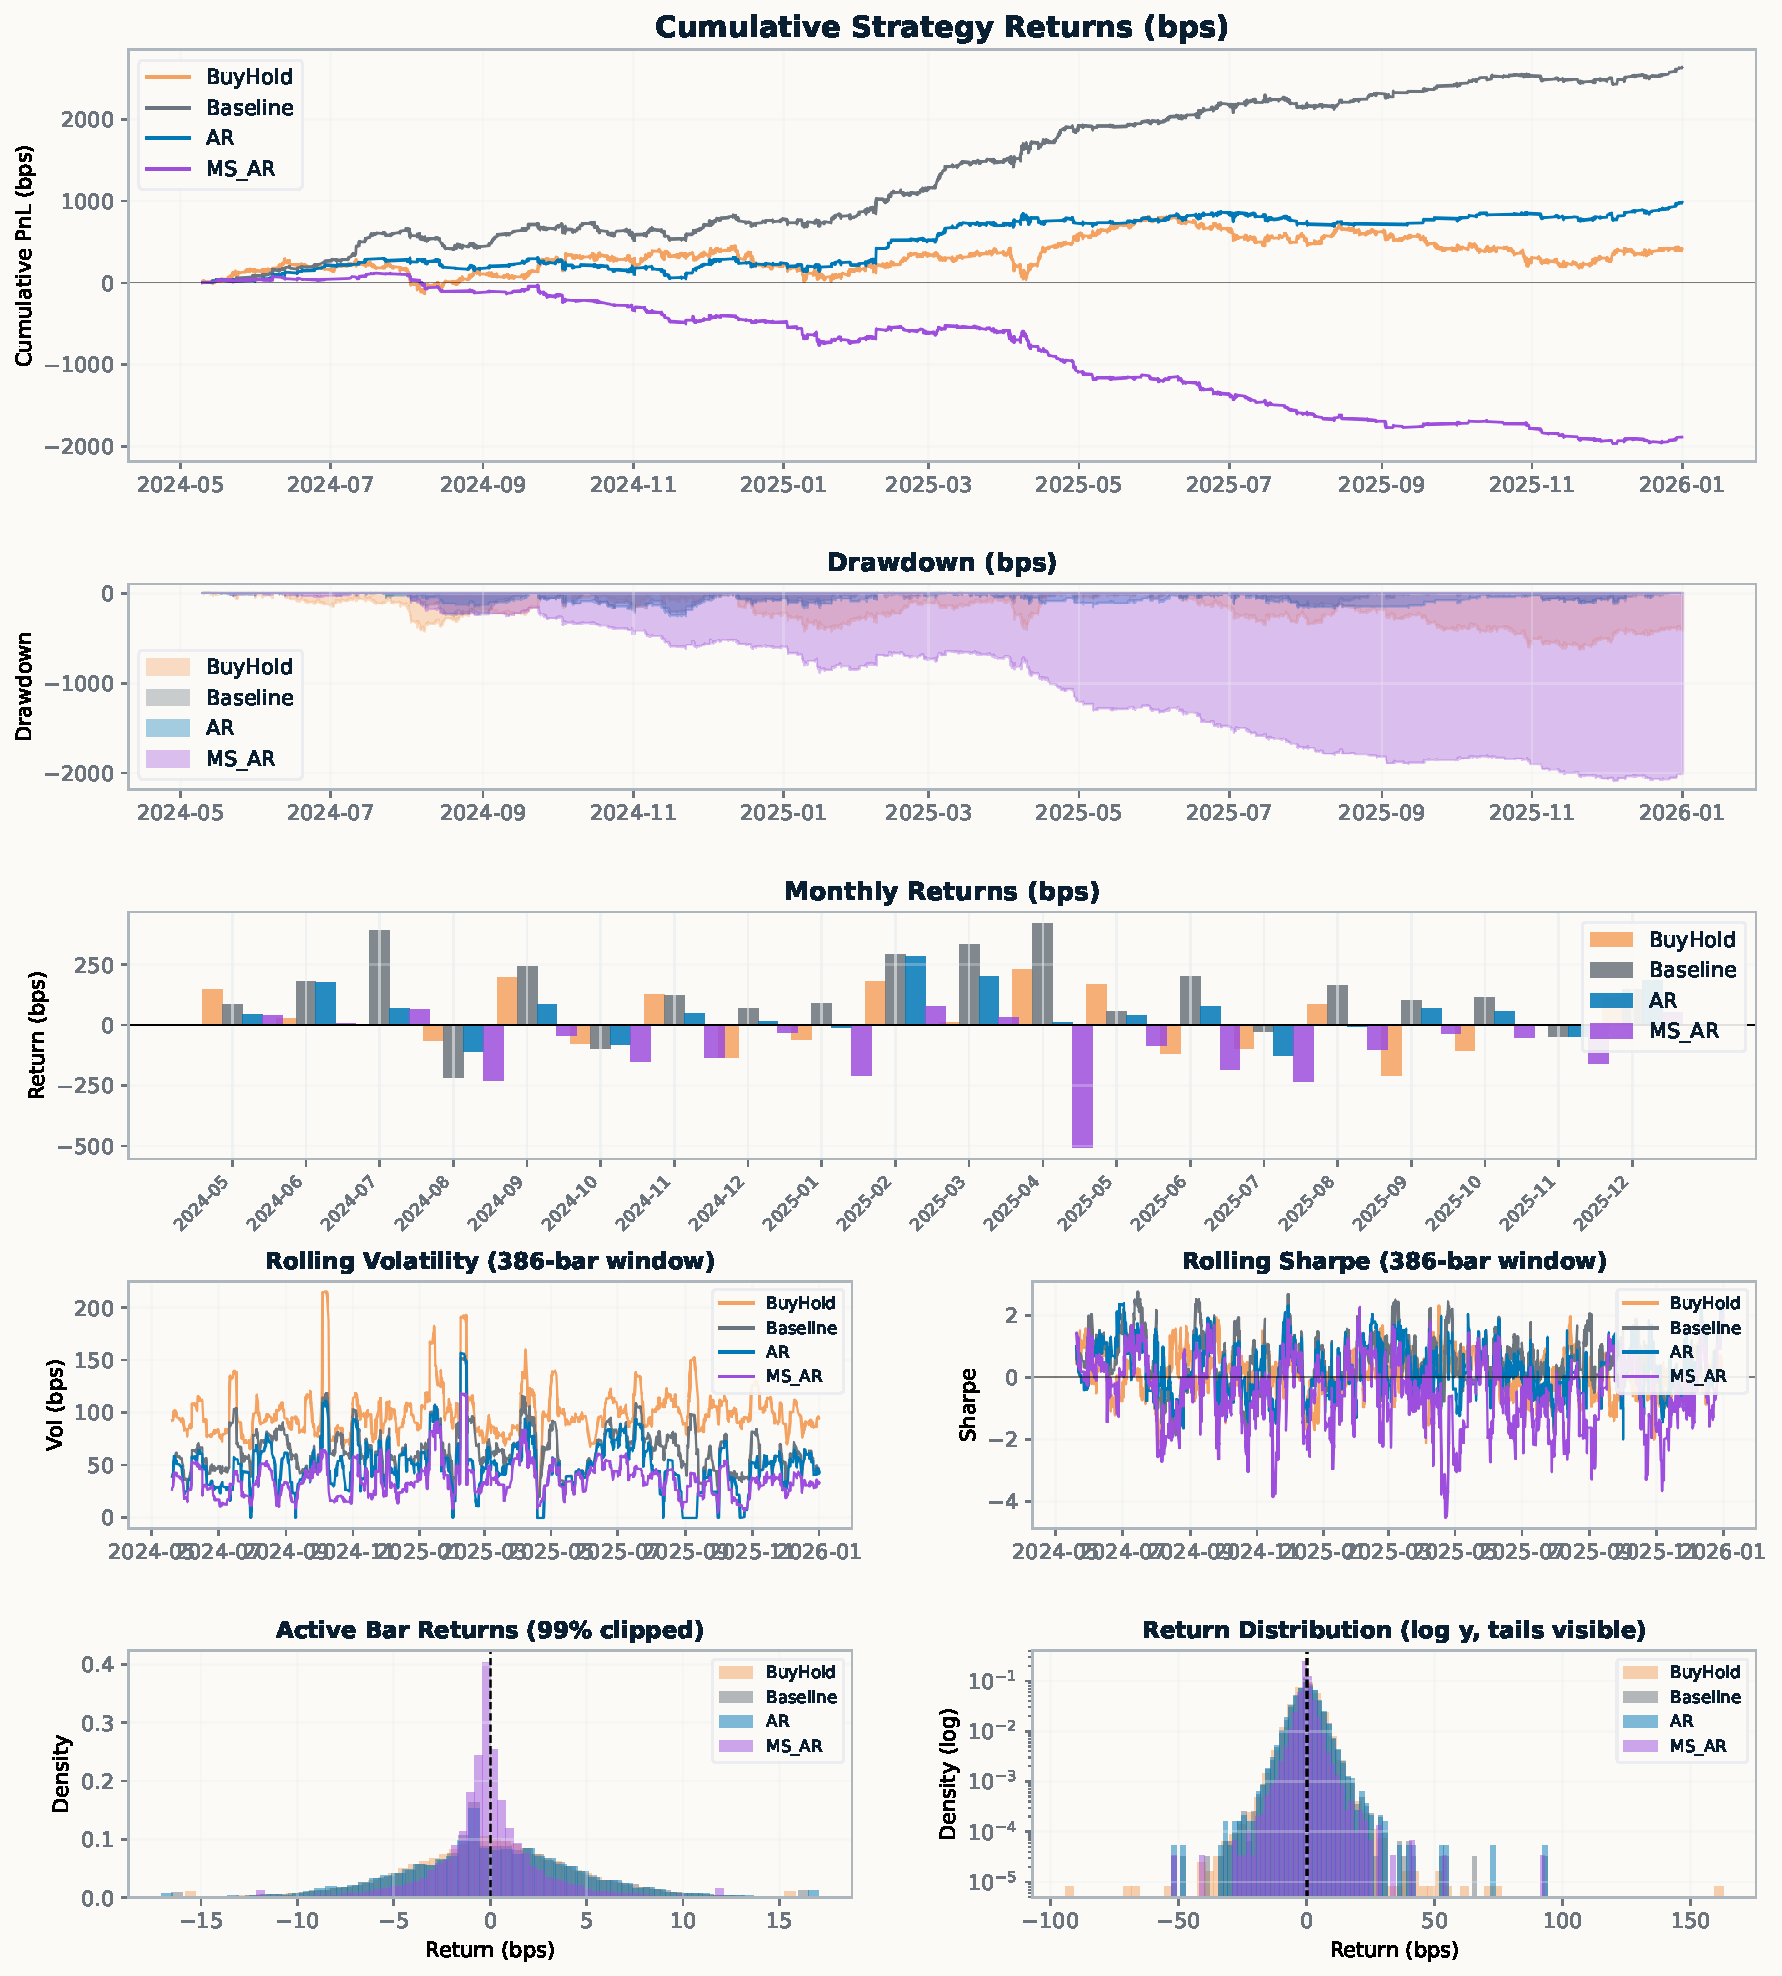
\includegraphics[width=\textwidth]{plots/GBPUSD_EURUSD_daily_performance.pdf}
    \caption{Daily backtest performance for GBPUSD/EURUSD across the baseline, AR, and Markov-switching AR strategies. The figure compares cumulative returns, drawdowns, monthly returns, rolling volatility, rolling Sharpe ratios, active-day return densities, and tail behaviour under the competing model specifications.}
    \label{fig:GBPUSD_EURUSD_daily_performance}
\end{figure}